\documentclass{simcenterdocumentation}
\usepackage[backend=biber]{biblatex}
%\usepackage{subfig}
\usepackage{amsmath}
\usepackage{bm}
\usepackage{subcaption}
\usepackage{multirow}
\usepackage{adjustbox}
\usepackage{cleveref}
\usepackage{longtable}
\usepackage{amssymb}

\usepackage{hhline}
\usepackage{color, colortbl}
\definecolor{lightgray}{HTML}{E5E4E2}

%% SETTING ENVIRONMENT FOR PYTHON CODE SNIPPETS %%%%%%%%%%%%%%%%%%%%%%%%%%%%%%% 
\usepackage[utf8]{inputenc}

\graphicspath{{../Common/}{.}} %Setting the graphicspath
\makeatletter % Search additional directories for inputs
\def\input@path{{../Common/}{.}}
%or: \def\input@path{{/path/to/folder/}{/path/to/other/folder/}}
\makeatother

%%%%%%%%%%%%%%%%%%%%%%%%%%%%%%%%%%%%%%%%%%%%%%%%%%%%%%%%%%%%%%%%%%%%%%%%%%%%%%% 

% To compile this file, run "latex/pdflatex codedoc", then "biber codedoc"
% (or "bibtex codedoc", if the output from latex asks for that instead),
% and then "latex/pdflatex codedoc" (without the quotes in each case).

% Double spacing, if you want it.  Do not use for the final copy. Can also specify
% draft as a document class option. This will generate double spacing and placeholders
% for title page and header images
%% \def\dsp{\def\baselinestretch{2.0}\large\normalsize}
%% \dsp

\bibliography{../Common/references}

\begin{document}

% Declarations for Front Matter
% Software title followed by optional second line
\title{WE-UQ\\ \Large The Wind Engineering with Uncertainty Quantification (WE-UQ) Application}
% Use superscripts to indicate author affiliations
\author{Frank McKenna$^{1}$, Jiawei Wan$^{3}$, Wael Elhaddad$^{1}$,\\Michael Gardner$^{1}$,  Peter McKenzie-Helnwein$^{2}$, and Ahsan Kareem$^3$}
%\author{Moe Howard$^{1,2}$ Larry Fine$^1$ Curly Howard$^2$}
\institutions{$^{1}$University of California, Berkeley \\$^{2}$University of Washington \\$^{3}$University of Notre Dame}
\softwarename{WE-UQ}
\softwareversion{2.0}
\softwarepage{https://simcenter.designsafe-ci.org/research-tools/we-uq-application/}

%%% DON'T MESS WITH THESE SETTINGS %%%%%%%%%%%%%%%%%%%%%%%%%%%%%%%%
\hypersetup{pageanchor=false}
\maketitle
\copyrightpage
\acknowledgments

\hypersetup{pageanchor=true}
\begin{frontmatter}

\pagestyle{plain}
{
  \renewcommand{\thispagestyle}[1]{}
  \tableofcontents
  \clearpage
  \listoffigures
  \clearpage
  \listoftables
}

\end{frontmatter}
\pagestyle{somewhatsimple}
%%%%%%%%%%%%%%%%%%%%%%%%%%%%%%%%%%%%%%%%%%%%%%%%%%%%%%%%%%%%%%%%%%%
% Create separate tex files for each chapter and provide them as inputs

\chapter{About}
\label{chap:about}
The intended audience for this tool is researchers and practitioners
interested in predicting the response of a structure to wind loading
events.\\

This open-source research application, the source code of which is
available at
the \href{https://github.com/NHERI-SimCenter/WE-UQ}{\texttt{\getsoftwarename{}}
Github page}, provides an application that can be used to predict the
response of a building subjected to wind events. The application
is focused on quantifying the uncertainties in the predicted response,
given the that the properties of the buildings and the wind
events are not known exactly, and that both the simulation software
and the user make simplifying assumptions in the numerical modeling of
that structure. In this application, the user is required to
characterize the uncertainties in the input. The application will,
after utilizing the users selected sampling method, provide
information that characterizes the uncertainties in the computed
response measures. As the computations to make these determinations
can be prohibitively expensive to perform on a user's local computer,
the user has the option to perform the computations remotely on the
Stampede2 supercomputer. Stampede2 is located at the Texas Advanced
Computing Center (TACC) and made available to the user through NHERI
DesignSafe, the cyberinfrastructure provider for the distributed NSF
funded Natural Hazards in Engineering Research Infrastructure (NHERI)
facility.\\

Whether running locally or remotely, the computations are performed,
as will be discussed in \Cref{chap:theory}, in a workflow
application. That is, the numerical simulations are actually performed
by a number of different applications. The \texttt{\getsoftwarename{}} backend software runs
these different applications for the user, taking the outputs from
some programs and providing them as inputs to others. The design of
the \texttt{\getsoftwarename{}} application is such that researchers are able to modify the
backend application to utilize their own application in the workflow
computations. This will ensure researchers are not limited to using
the default applications we provide and will be enthused to provide
their own applications for others to use. \\

This document covers Version \getsoftwareversion{} of the tool. Users are
encouraged to comment on what additional features and capabilities
they would like to see in this application. These requests and
feedback can be submitted through an anonymous \insertsurveylink{user
survey}; we greatly appreciate any input you have. If there are
features you want, chances are many of your colleagues also would
benefit from them. Users are encouraged to review
\Cref{chap:requirements} to see what features are planned for this
application.


\chapter{Installation Instructions}
\label{chap:installation}
All SimCenter applications are available at the \href{https://simcenter.designsafe-ci.org/research-tools/overview/}{SimCenter
website} under \emph{Research Tools}. The following sections outline
the steps necessary to download and install the \texttt{\getsoftwarename{}}
application. The SimCenter applications require that you install a
number of other applications that are needed to run the workflows on
your local machine as well as at DesignSafe. \\


%===============================================================================
\section{Download the Application}
%===============================================================================

% \subsection{Download the Application Files}

To download the \texttt{\getsoftwarename{}} application navigate to
the \getsoftwarepage{\texttt{\getsoftwarename{}} page} and click on
the \emph{Download App \& User Manual} link on the right side of the
page. As shown in \Cref{fig:app_choose_file}, this will bring you to another page which contains a list of downloadable files and directories.

\softwareSwitch{PBE}{
\begin{figure}[!htbp]
  \centering {
    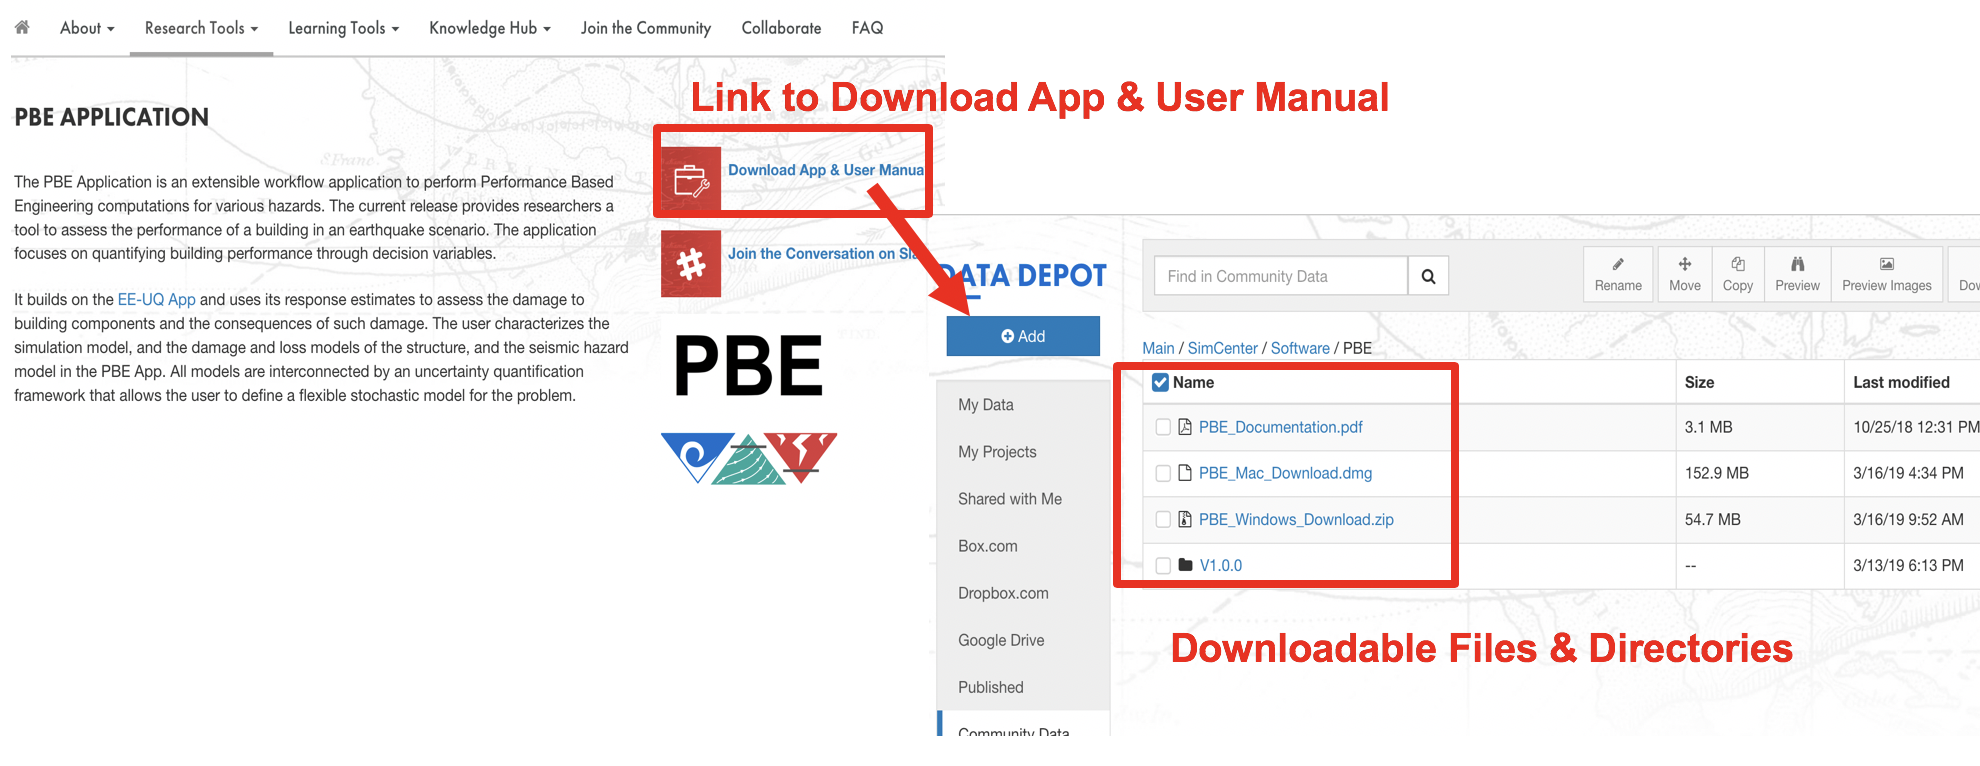
\includegraphics[width=0.95\textwidth]
    {installation/figures/pbeDownload.png} }
  \caption{Download Application}
  \label{fig:app_choose_file}
\end{figure}
}{}

\softwareSwitch{EE-UQ}{
\begin{figure}[!htbp]
  \centering {
    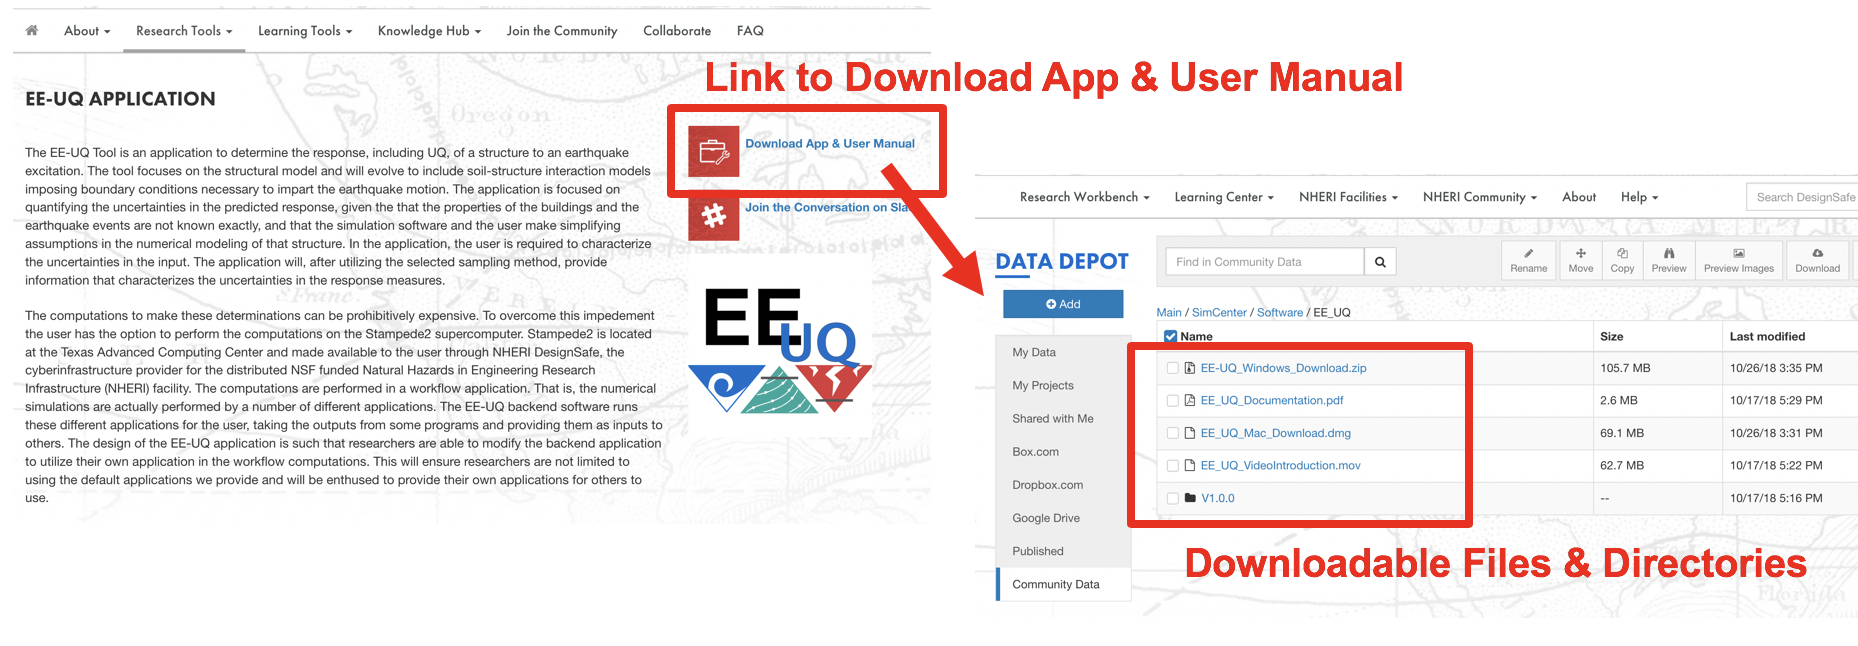
\includegraphics[width=0.95\textwidth]
    {installation/figures/eeDownload.png} }
  \caption{Download Application}
  \label{fig:app_choose_file}
\end{figure}
}{}

\softwareSwitch{WE-UQ}{
\begin{figure}[!htbp]
  \centering {
    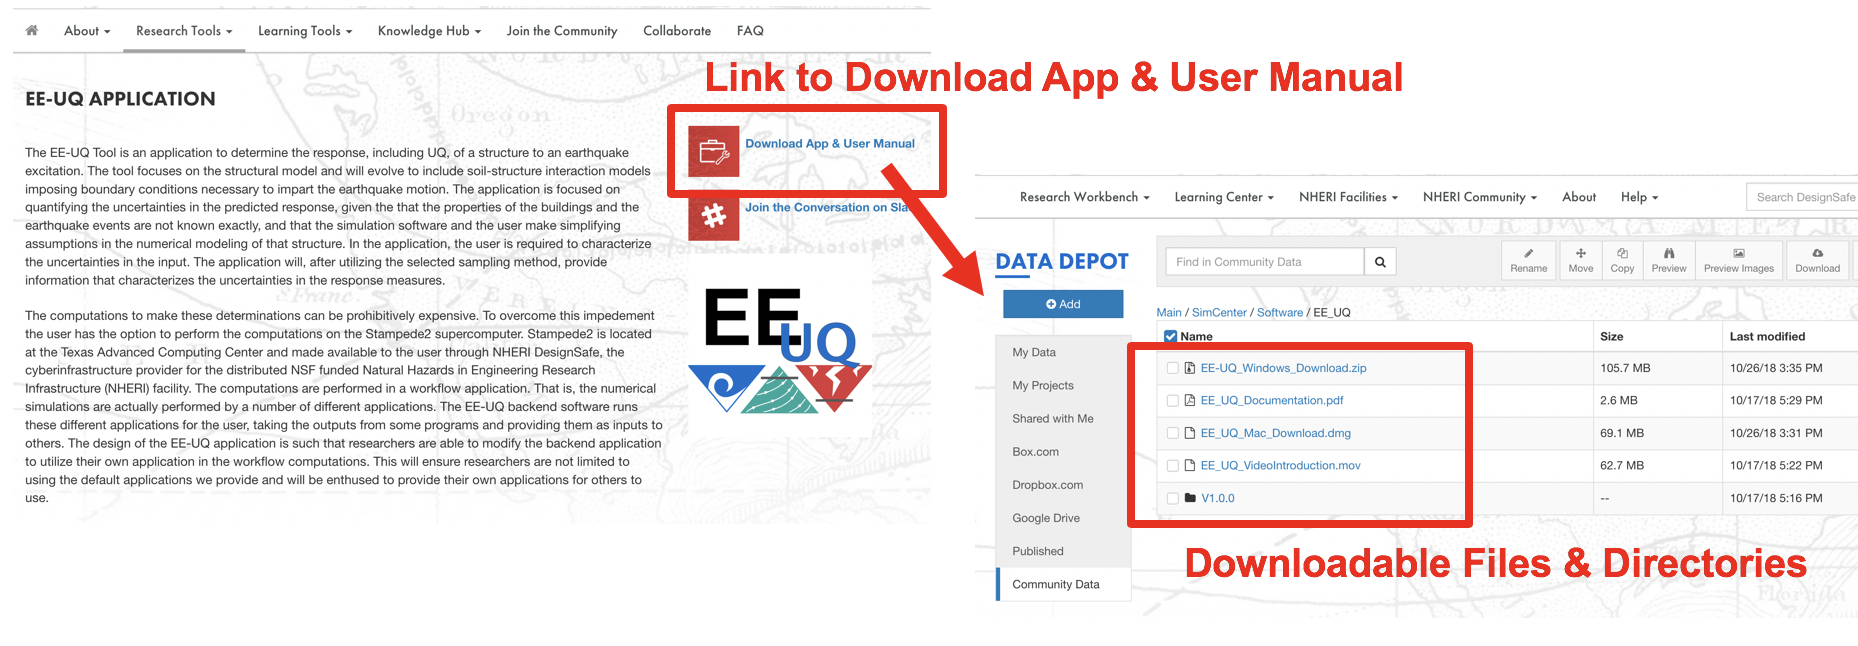
\includegraphics[width=0.95\textwidth]
    {installation/figures/eeDownload.png} }
  \caption{Download Application}
  \label{fig:app_choose_file}
\end{figure}
}{}


There are at least four files available for download from this page: 
\begin{enumerate}
    \item The PDF file is the User Manual that you are reading now.
    \item The MOV file is an video that provides an introduction to the usage of the application.
    \item The ZIP file is an archive that contains the application files for a Windows operating system.
    \item The DMG file is an archive that contains the application files for a Mac OS X operating system.
\end{enumerate}

To download the \texttt{\getsoftwarename{}} application click on the link for
the appropriate file for your operating system and then click on the
Download button at bottom right corner of the ensuing pop-up window. 
Unpackage the application from the downloaded
file and place it in a location on your filesystem. On Windows, we
recommend that you create a \texttt{C:/SimCenter/\getsoftwarename{}}
directory and extract the contents of the \texttt{ZIP} archive
there. It is also recommended to run the included installer for Visual C/C++ runtime library(vc\_redist.x64.exe).
If you use a Mac we recommend you copy the application to either your
home folder or your Desktop folder. You are free to place the
applications anywhere you wish, you will need to make the
appropriate adjustments with the following instructions if you do so. \\

Now test that the application starts. To do this navigate to
the location where you placed the application and open it. You should
see the user interface (UI) shown in \Cref{fig:app_UI} after
starting the application. Now Quit the application. Additional steps are required before 
computations can be performed.\\

\softwareSwitch{PBE}{
\begin{figure}[!htbp]
  \centering {
    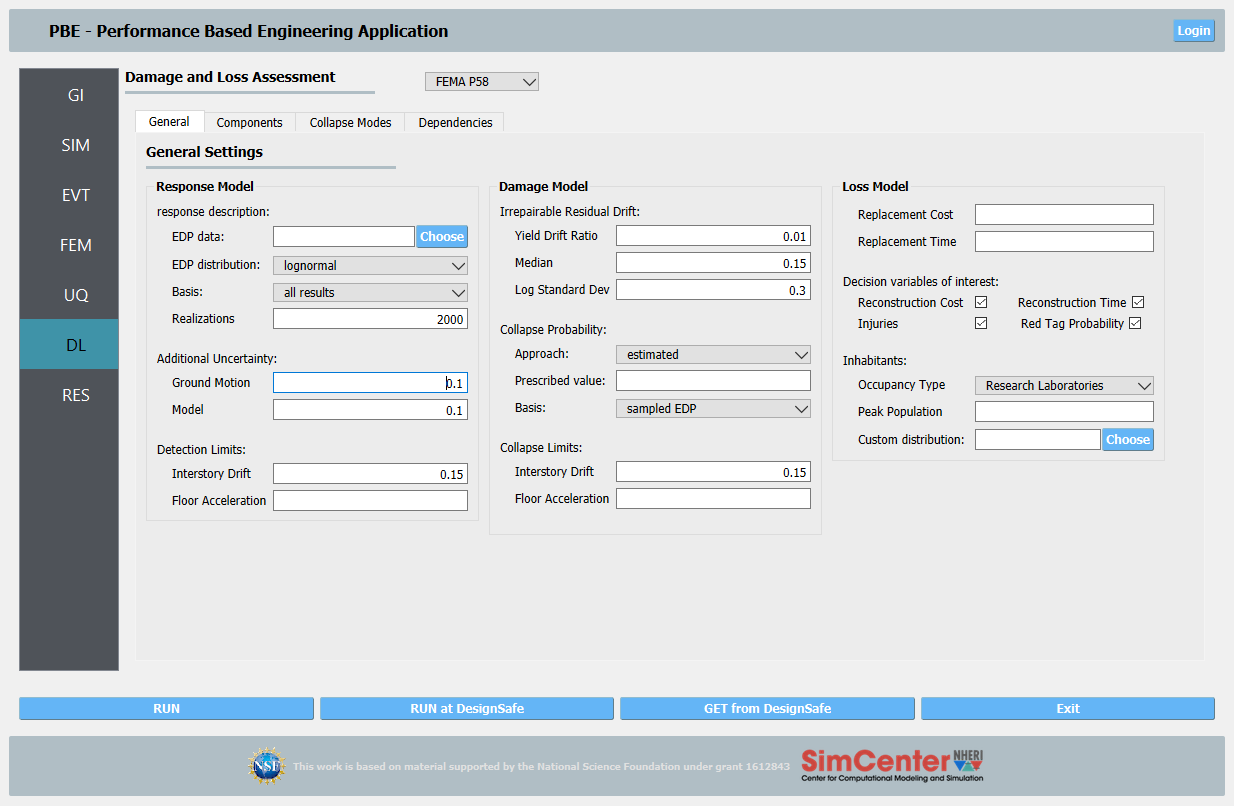
\includegraphics[width=0.95\textwidth]
    {installation/figures/PBE.png} }
  \caption{PBE Application on Startup}
  \label{fig:app_UI}
\end{figure}
}{}

\softwareSwitch{EE-UQ}{
\begin{figure}[!htbp]
  \centering {
    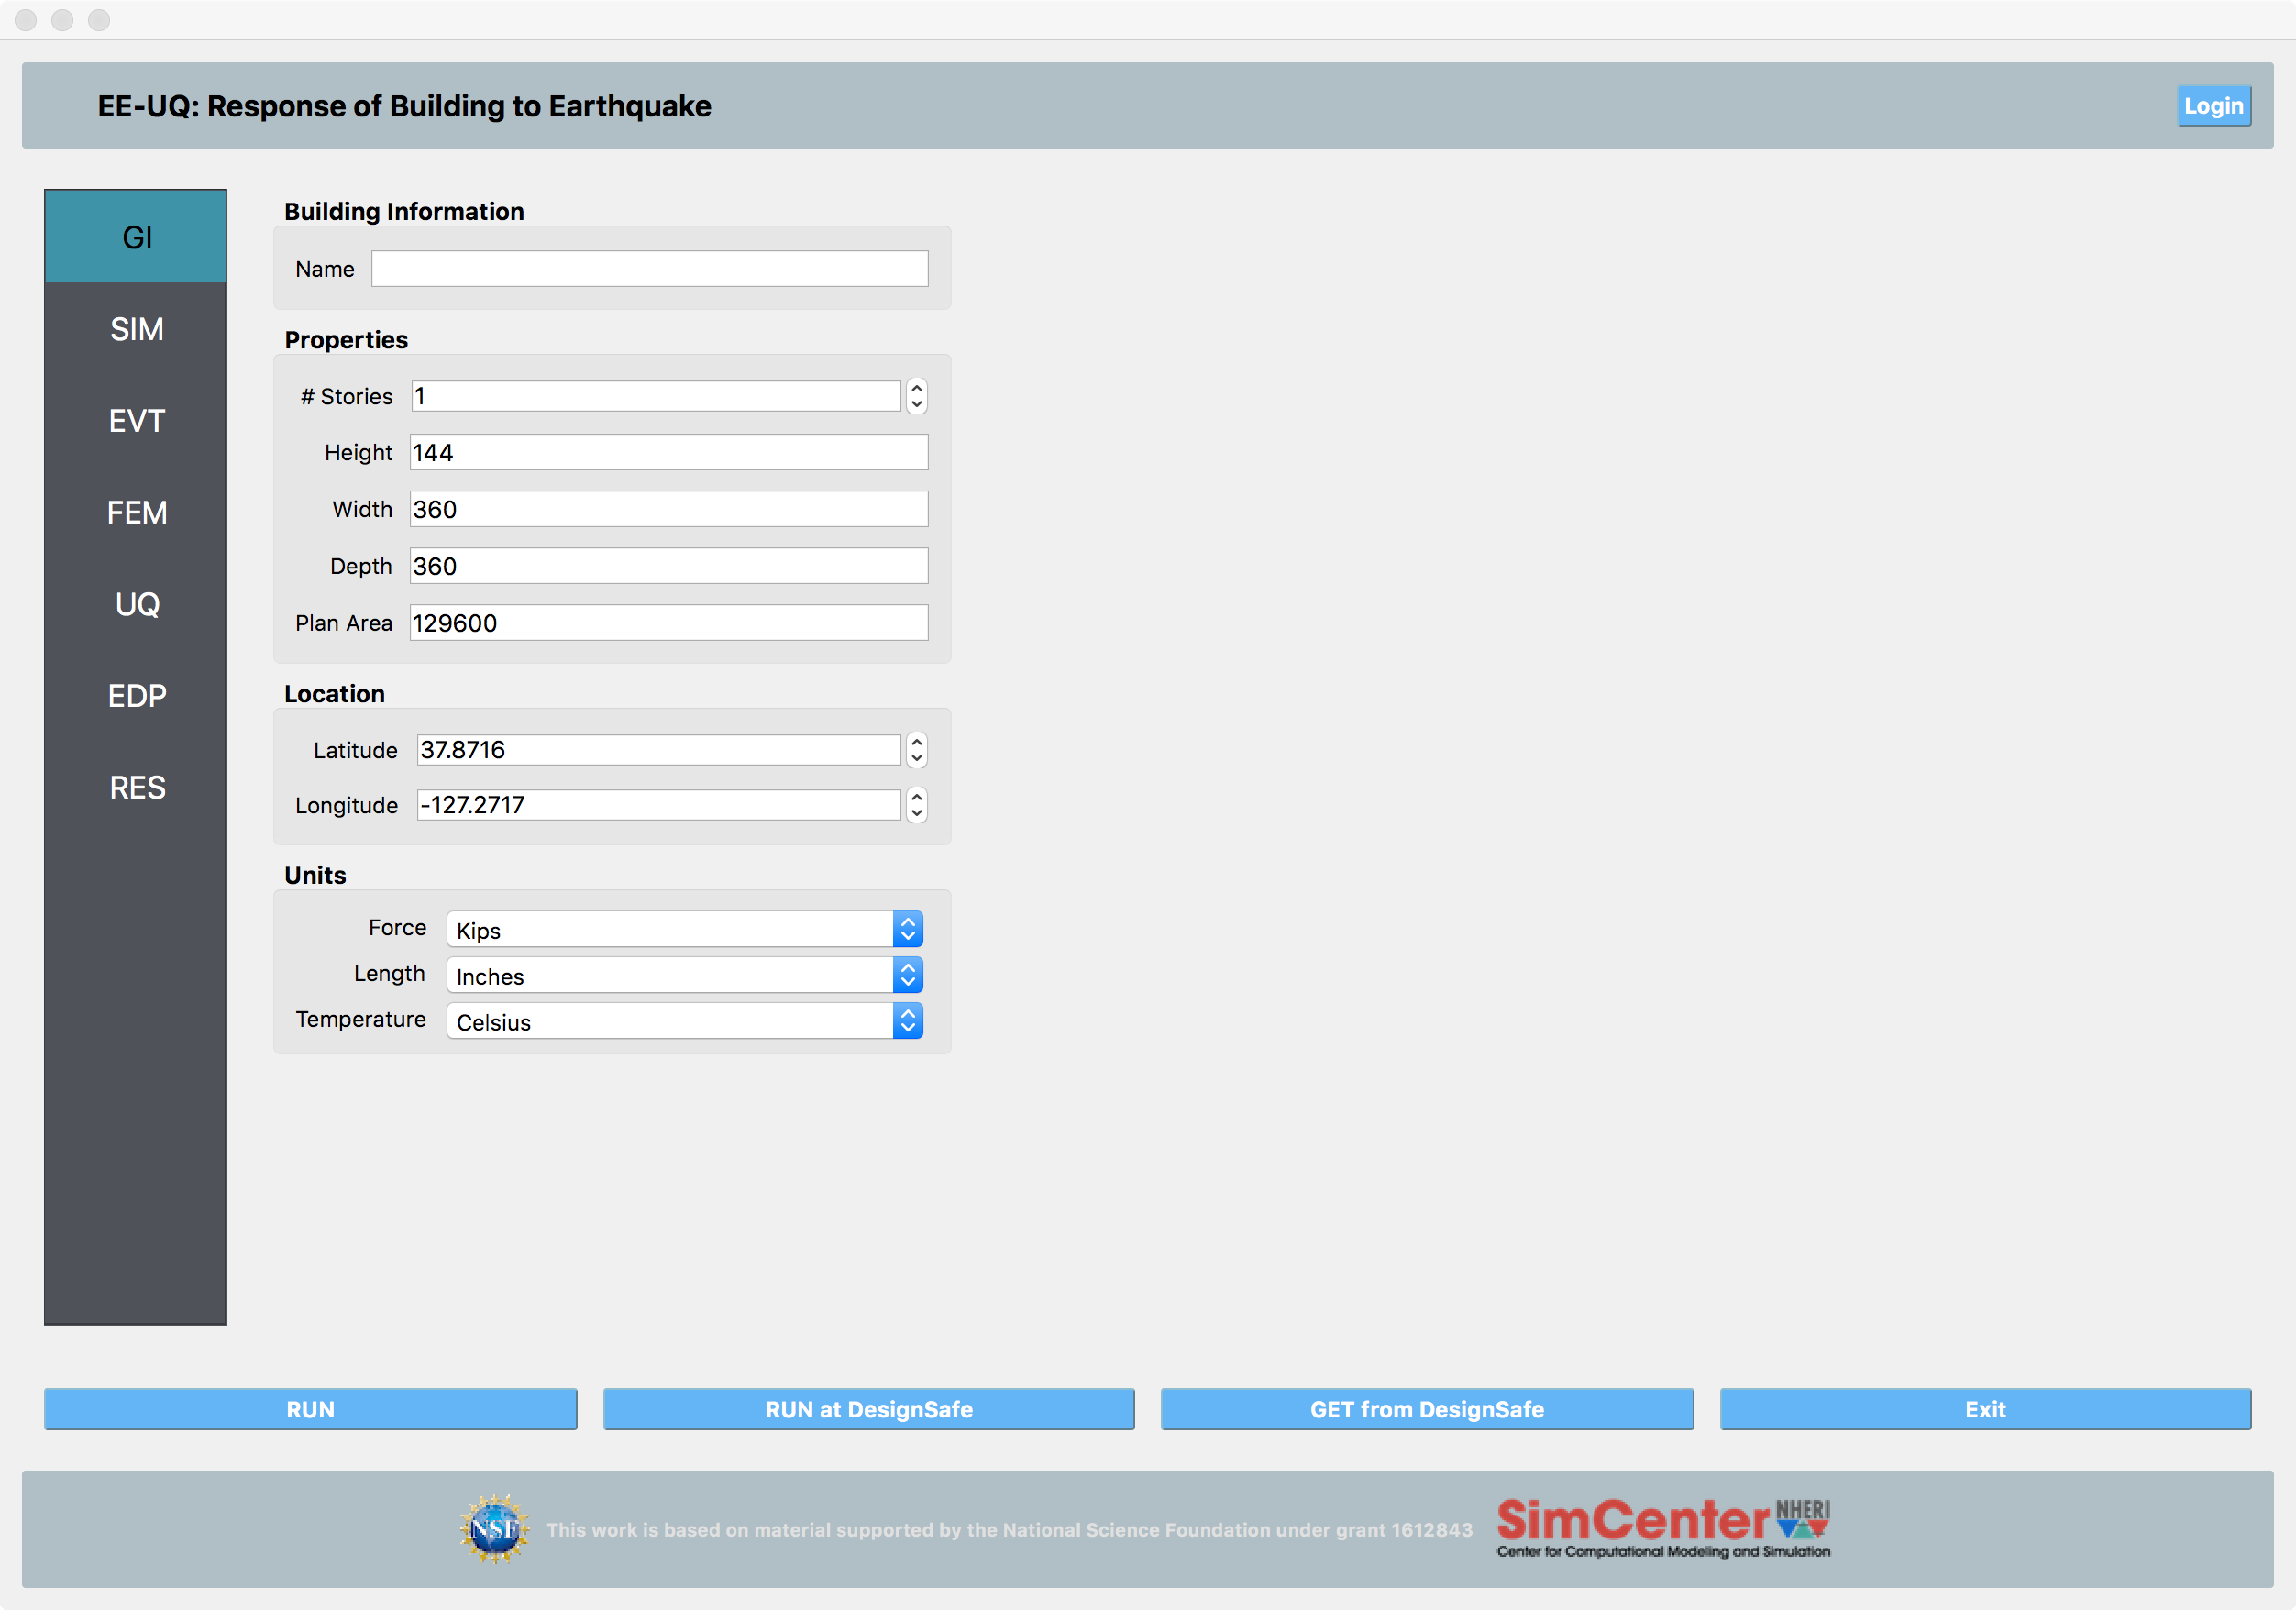
\includegraphics[width=0.95\textwidth]
    {installation/figures/EE-UQ.png} }
  \caption{EE-UQ Application on Startup}
  \label{fig:app_UI}
\end{figure}
}{}

\softwareSwitch{WE-UQ}{
\begin{figure}[!htbp]
  \centering {
    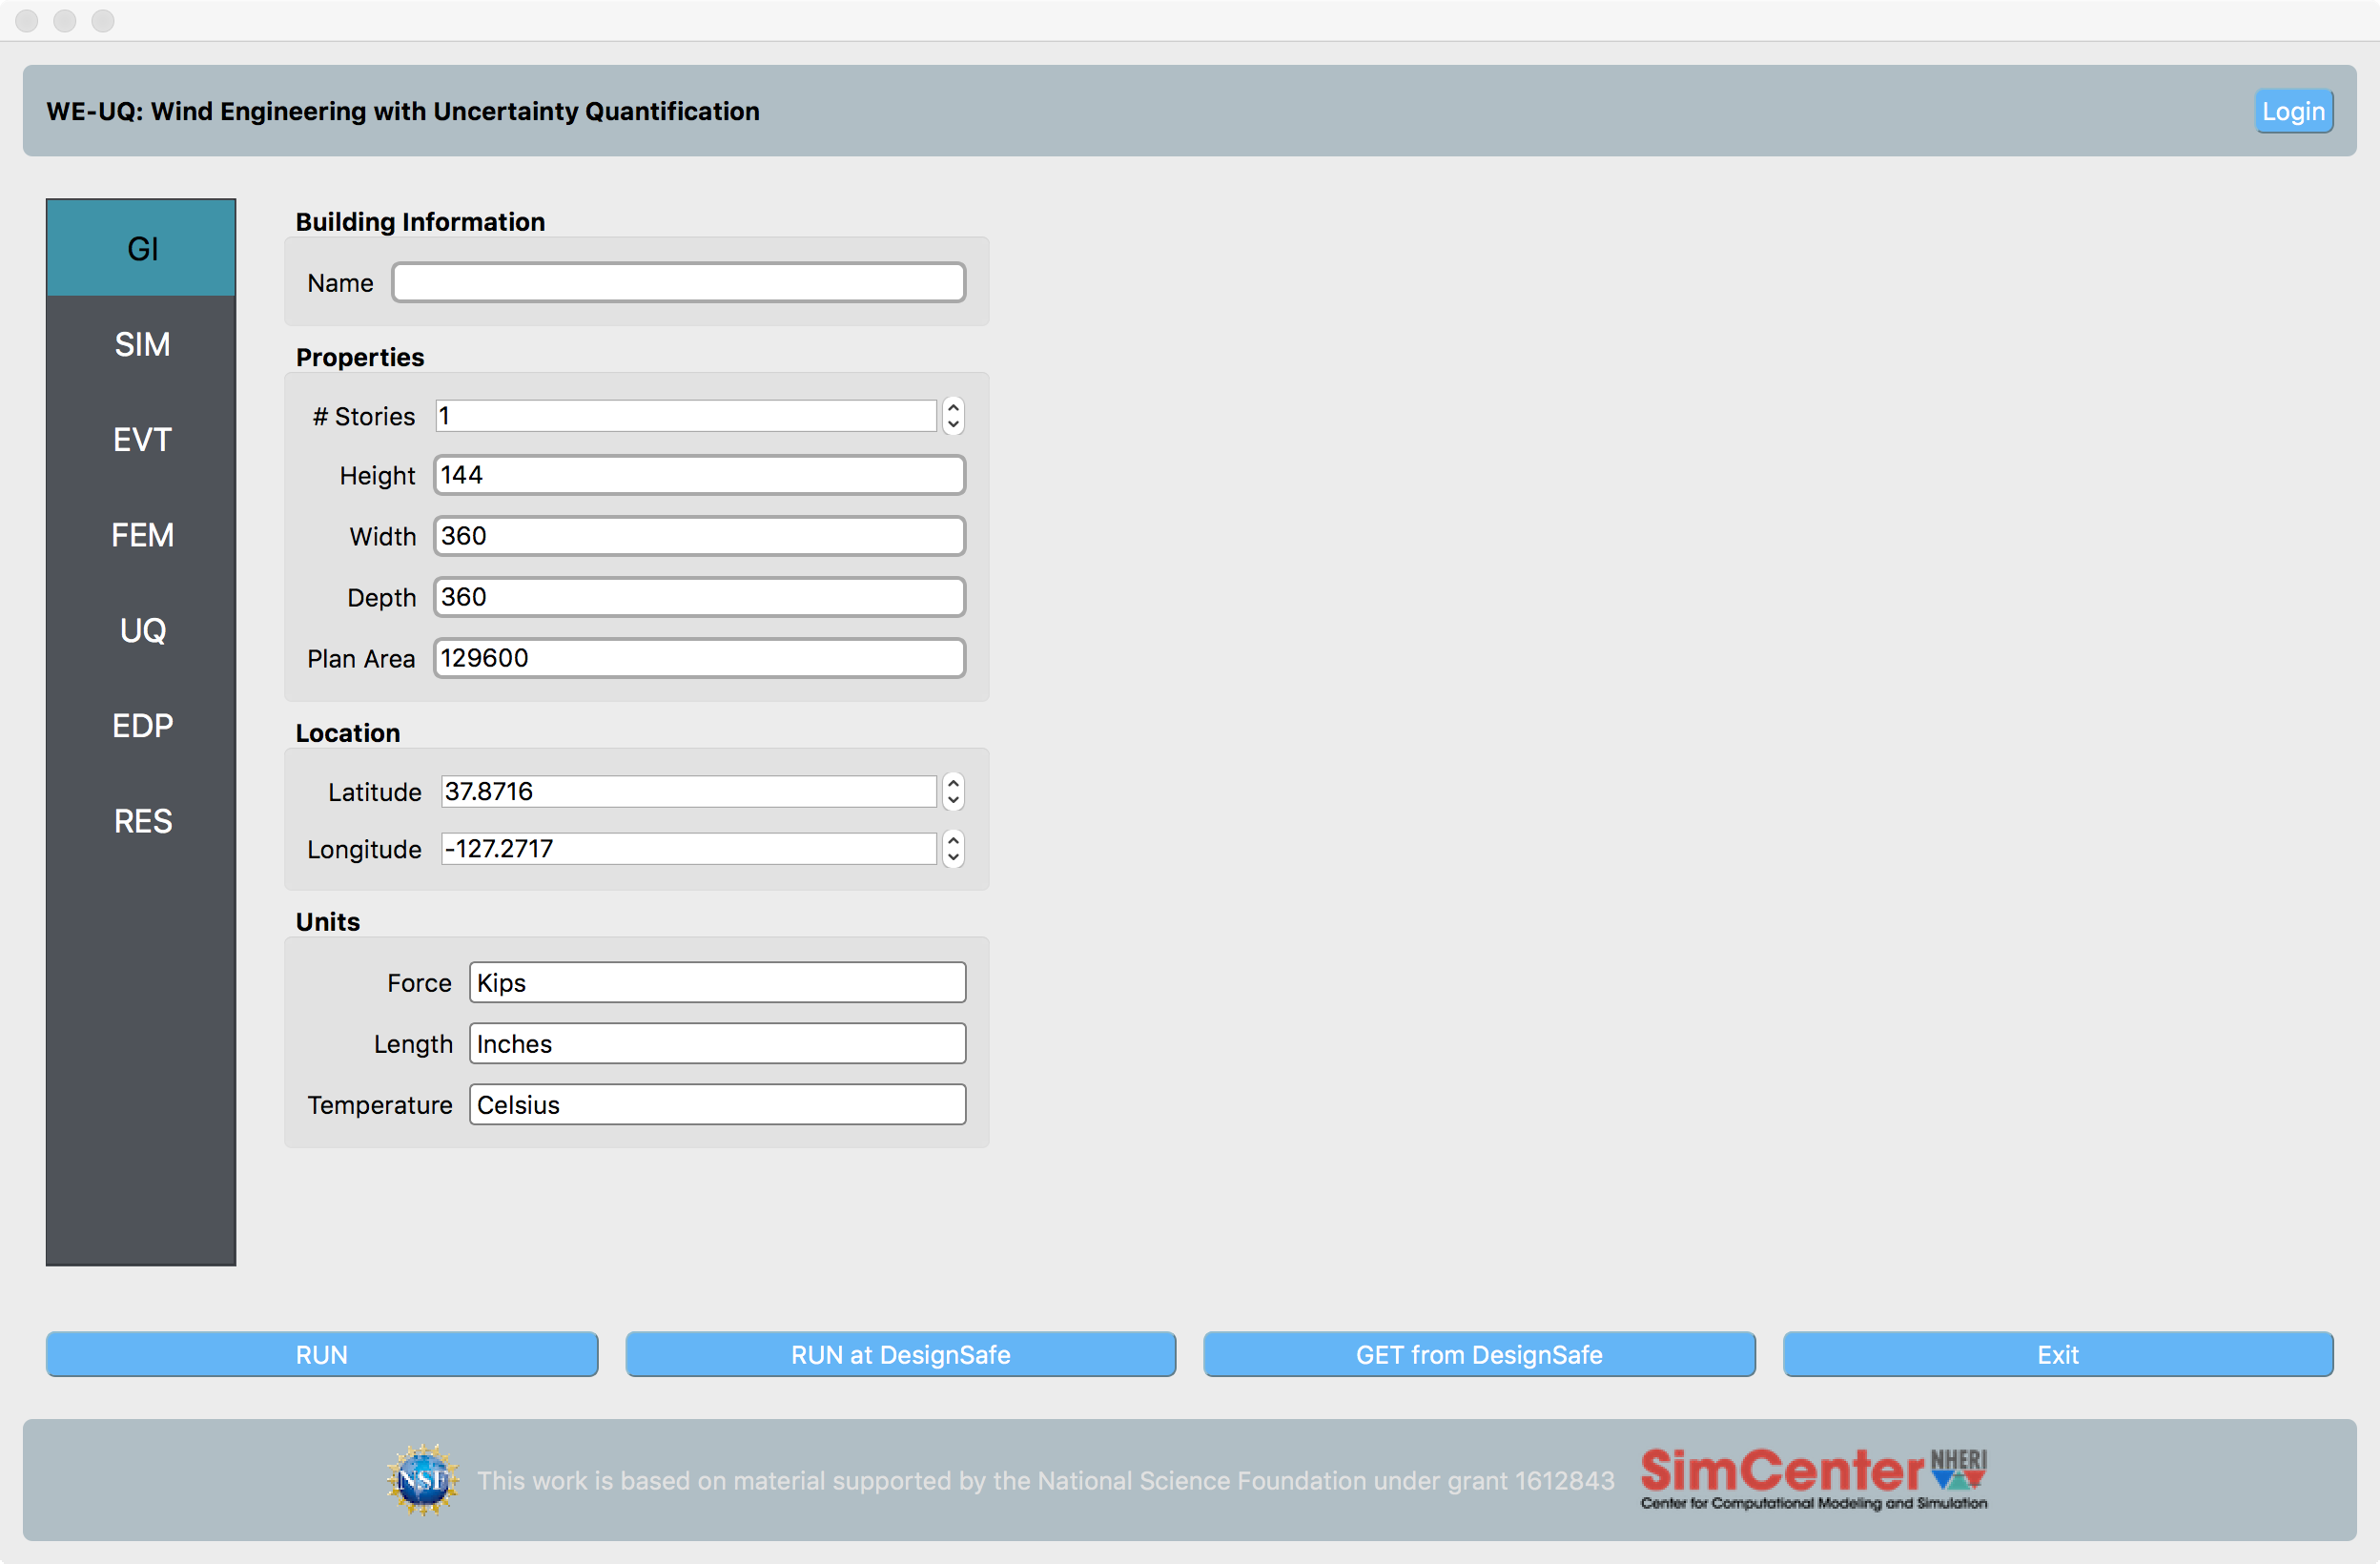
\includegraphics[width=0.95\textwidth]
    {installation/figures/WE-UQ.png} }
  \caption{WE-UQ Application on Startup}
  \label{fig:app_UI}
\end{figure}
}{}


\begin{enumerate}
\item The SimCenter is not recognized as either a Windows or an Apple vendor. Our applications are not recognized by the operating system as being signed. Consequently, you may receive a warning message when you start the \texttt{\getsoftwarename{}} application for the first time.
\item  On a Mac you will need to right click on the .dmg file to open it. The UI will not start correctly while in the DMG file, you need to open the .dmg file and then copy the \texttt{\getsoftwarename{}} application to your Documents or Desktop folder. You can then move the .dmg file to the trash or eject it after this has been done.
\item  The \texttt{\getsoftwarename{}} application requires additional software outlined in next subsections to work properly. Even if the application starts correctly, it will not run the simulations until these software, outlined in the next section, are installed.
\end{enumerate}


%===============================================================================
\section{Set up Python}
%===============================================================================

The SimCenter workflow applications are managed by Python
scripts. These are required to prepare the input data for running
analyses either remotely on DesignSafe or locally. Consequently, the user must have Python
installed on their machine and have the appropriate environment
variables set so that the UI can run these applications.

\subsection{Install Python}

SimCEnter products require Python version 3.7.
SimCenter products require Python version 3.7 or above be installed on your machine as January 2020 marks the end of life for Python 2.7. Our tools were tested with versions up to Python 3.7.5; we recommend using that version.


\begin{enumerate}
\item Windows:

If you have not yet installed Python 3.7, we recommend installing from \href{https://www.python.org/downloads/windows}{Python.org}. We recommend installing using the \texttt{Windows x86-64 executable installer}. NOTE: At time of writing Python 3.8.0 release will fail to install scipy on Windows 10 and should thus not be installed.

Allow the installer to change your system environment variables so that the install directory is added to your PATH. 

Once Python is installed, you need to extend it by installing the following packages: \texttt{numpy}, \texttt{scipy}, and \texttt{pandas}. To install these packages open a \href{https://www.howtogeek.com/194041/how-to-open-the-command-prompt-as-administrator-in-windows-8.1/}{terminal window as an Admin user} and in that window type the following instructions:

\begin{verbatim}
pip install numpy
pip install scipy
pip install pandas
\end{verbatim}

\item Mac

The Mac comes with Python pre-installed, which is currently the somewhat 
dated version 2.7. We recommend installing Python 3.7 from 
\href{https://www.python.org/downloads/}{Python.org}. We recommend installing using the 
\texttt {macOS 64-bit installer}. The installer will place a python3 executable in your /usr/local/bin directory, whose location should be on your system PATH.

Once Python is installed, you need to extend it by installing the following packages: \texttt{numpy}, \texttt{scipy}, and \texttt{pandas}. To install these packages, start a terminal window and type the following instructions:

\begin{verbatim}
pip3 install numpy
pip3 install scipy
pip3 install pandas
\end{verbatim}

Notes: 
\begin{enumerate}
\item To start a terminal window you can use the spotlight app (magnifying glass at the top right corner of the desktop). Start the spotlight app and type in terminal. The terminal application should appear as the top hit. Click on it to start it.
\item In the File/Preferences within the \texttt{\getsoftwarename{}} App make sure that python3 appears under External Applications / Python. If you used older versions of SimCenter tools this was the default.
\end{enumerate}
\end{enumerate}

\subsection{Test Python}
%===============================================================================

Test if the python environment is set up properly by
executing \texttt{python} in a terminal window. After Python starts,
test if the packages are installed by executing \texttt{import
numpy}, \texttt{import scipy}, and \texttt{import pandas}. You will
receive an error message if a pacakage is missing. If no error
appears, the terminal should look similar
to \Cref{fig:python_test}. Exit Python by executing
the \texttt{exit()} command.

\begin{figure}[!htbp]
  \centering {
    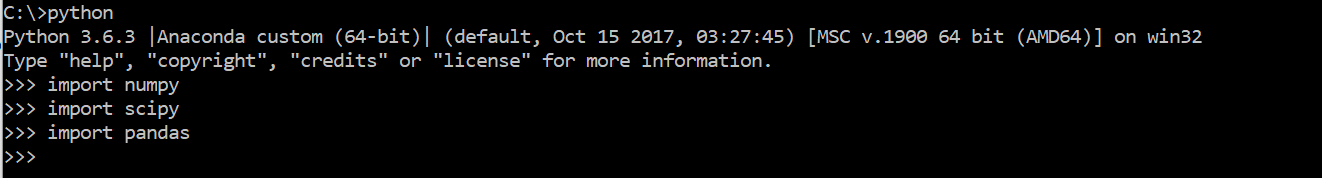
\includegraphics[width=0.8\textwidth]
    {installation/figures/python_test.png} }
  \caption{Testing the Python environment.}
  \label{fig:python_test}
\end{figure}

%===============================================================================
\section{Set up for Running Workflows Locally}\label{setup}
%===============================================================================

To run the workflows locally, the backend python application needs
publicly available software to also be installed on your
machine. These software applications need to be installed and
configured on your operating system. If you do not plan to run the
workflows locally, you will not need these applications.

\subsection{Install \texttt{OpenSees}}
%===============================================================================

\href{http://opensees.berkeley.edu}{\texttt{OpenSees}} is an open-source finite element application publicly available for download from its \href{http://opensees.berkeley.edu/OpenSees/user/download.php}{download page}. \texttt{OpenSees} installation requires the user install both \texttt{OpenSees} and \texttt{Tcl}.  If you have never downloaded \texttt{OpenSees} before, you will need to register your e-mail to gain access. After registration, you can proceed to the download page by entering your email address and clicking the Submit button. The Windows and Mac downloads are in different locations on the download page, with the appropriate Tcl installer beside the \texttt{OpenSees} link; see \Cref{fig:openseesDownload}

\begin{figure}[!htbp]
  \centering {
    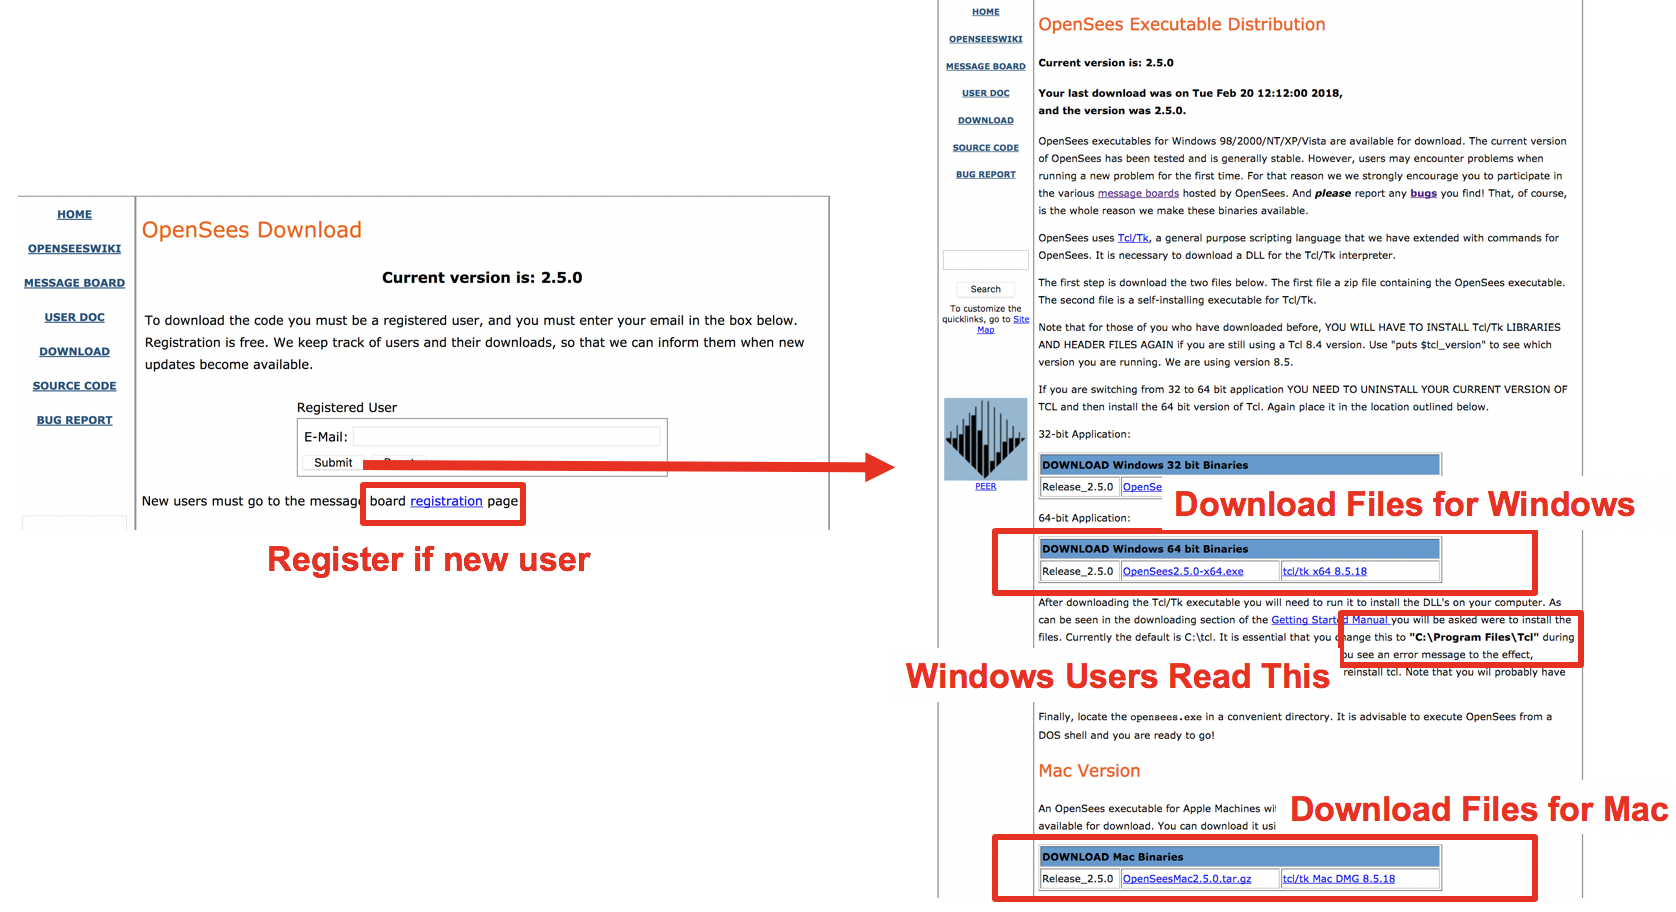
\includegraphics[width=\textwidth]
    {installation/figures/openseesDownload.png} }
  \caption{Downloading OpenSees}
  \label{fig:openseesDownload}
\end{figure}

Follow the instructions on the download page to install \texttt{Tcl}
(\Cref{fig:openseesDownload}). On Windows, you must select the Custom option for installton and you must specify
the installtion directory as \texttt{C:\textbackslash Program Files\textbackslash Tcl}, 
which is not the default. \\

After \texttt{Tcl} is installed, we recommend you put \texttt{OpenSees} in
the \texttt{C:/SimCenter/OpenSees} folder on Windows and in
a \texttt{/usr/local/OpenSees} directory on the Mac (If you use finder
on Mac to do navigation, use command-shift-G in Finder and specify
/usr/local as the folder to go to. Create a new folder \texttt{OpenSees}
and copy the \texttt{OpenSees} application to this folder).\\


Now you need to add the \texttt{OpenSees} folder to the
system \texttt{PATH} environment variable to allow the SimCenter
workflow applications to find the \texttt{OpenSees} executable on your
computer. The steps to do this depend on your operating system:

\begin{enumerate}
\item Windows: To add a folder to the \texttt{PATH} on Windows (\Cref{fig:add_env_path}):

\begin{figure}[!htbp]
  \centering {
    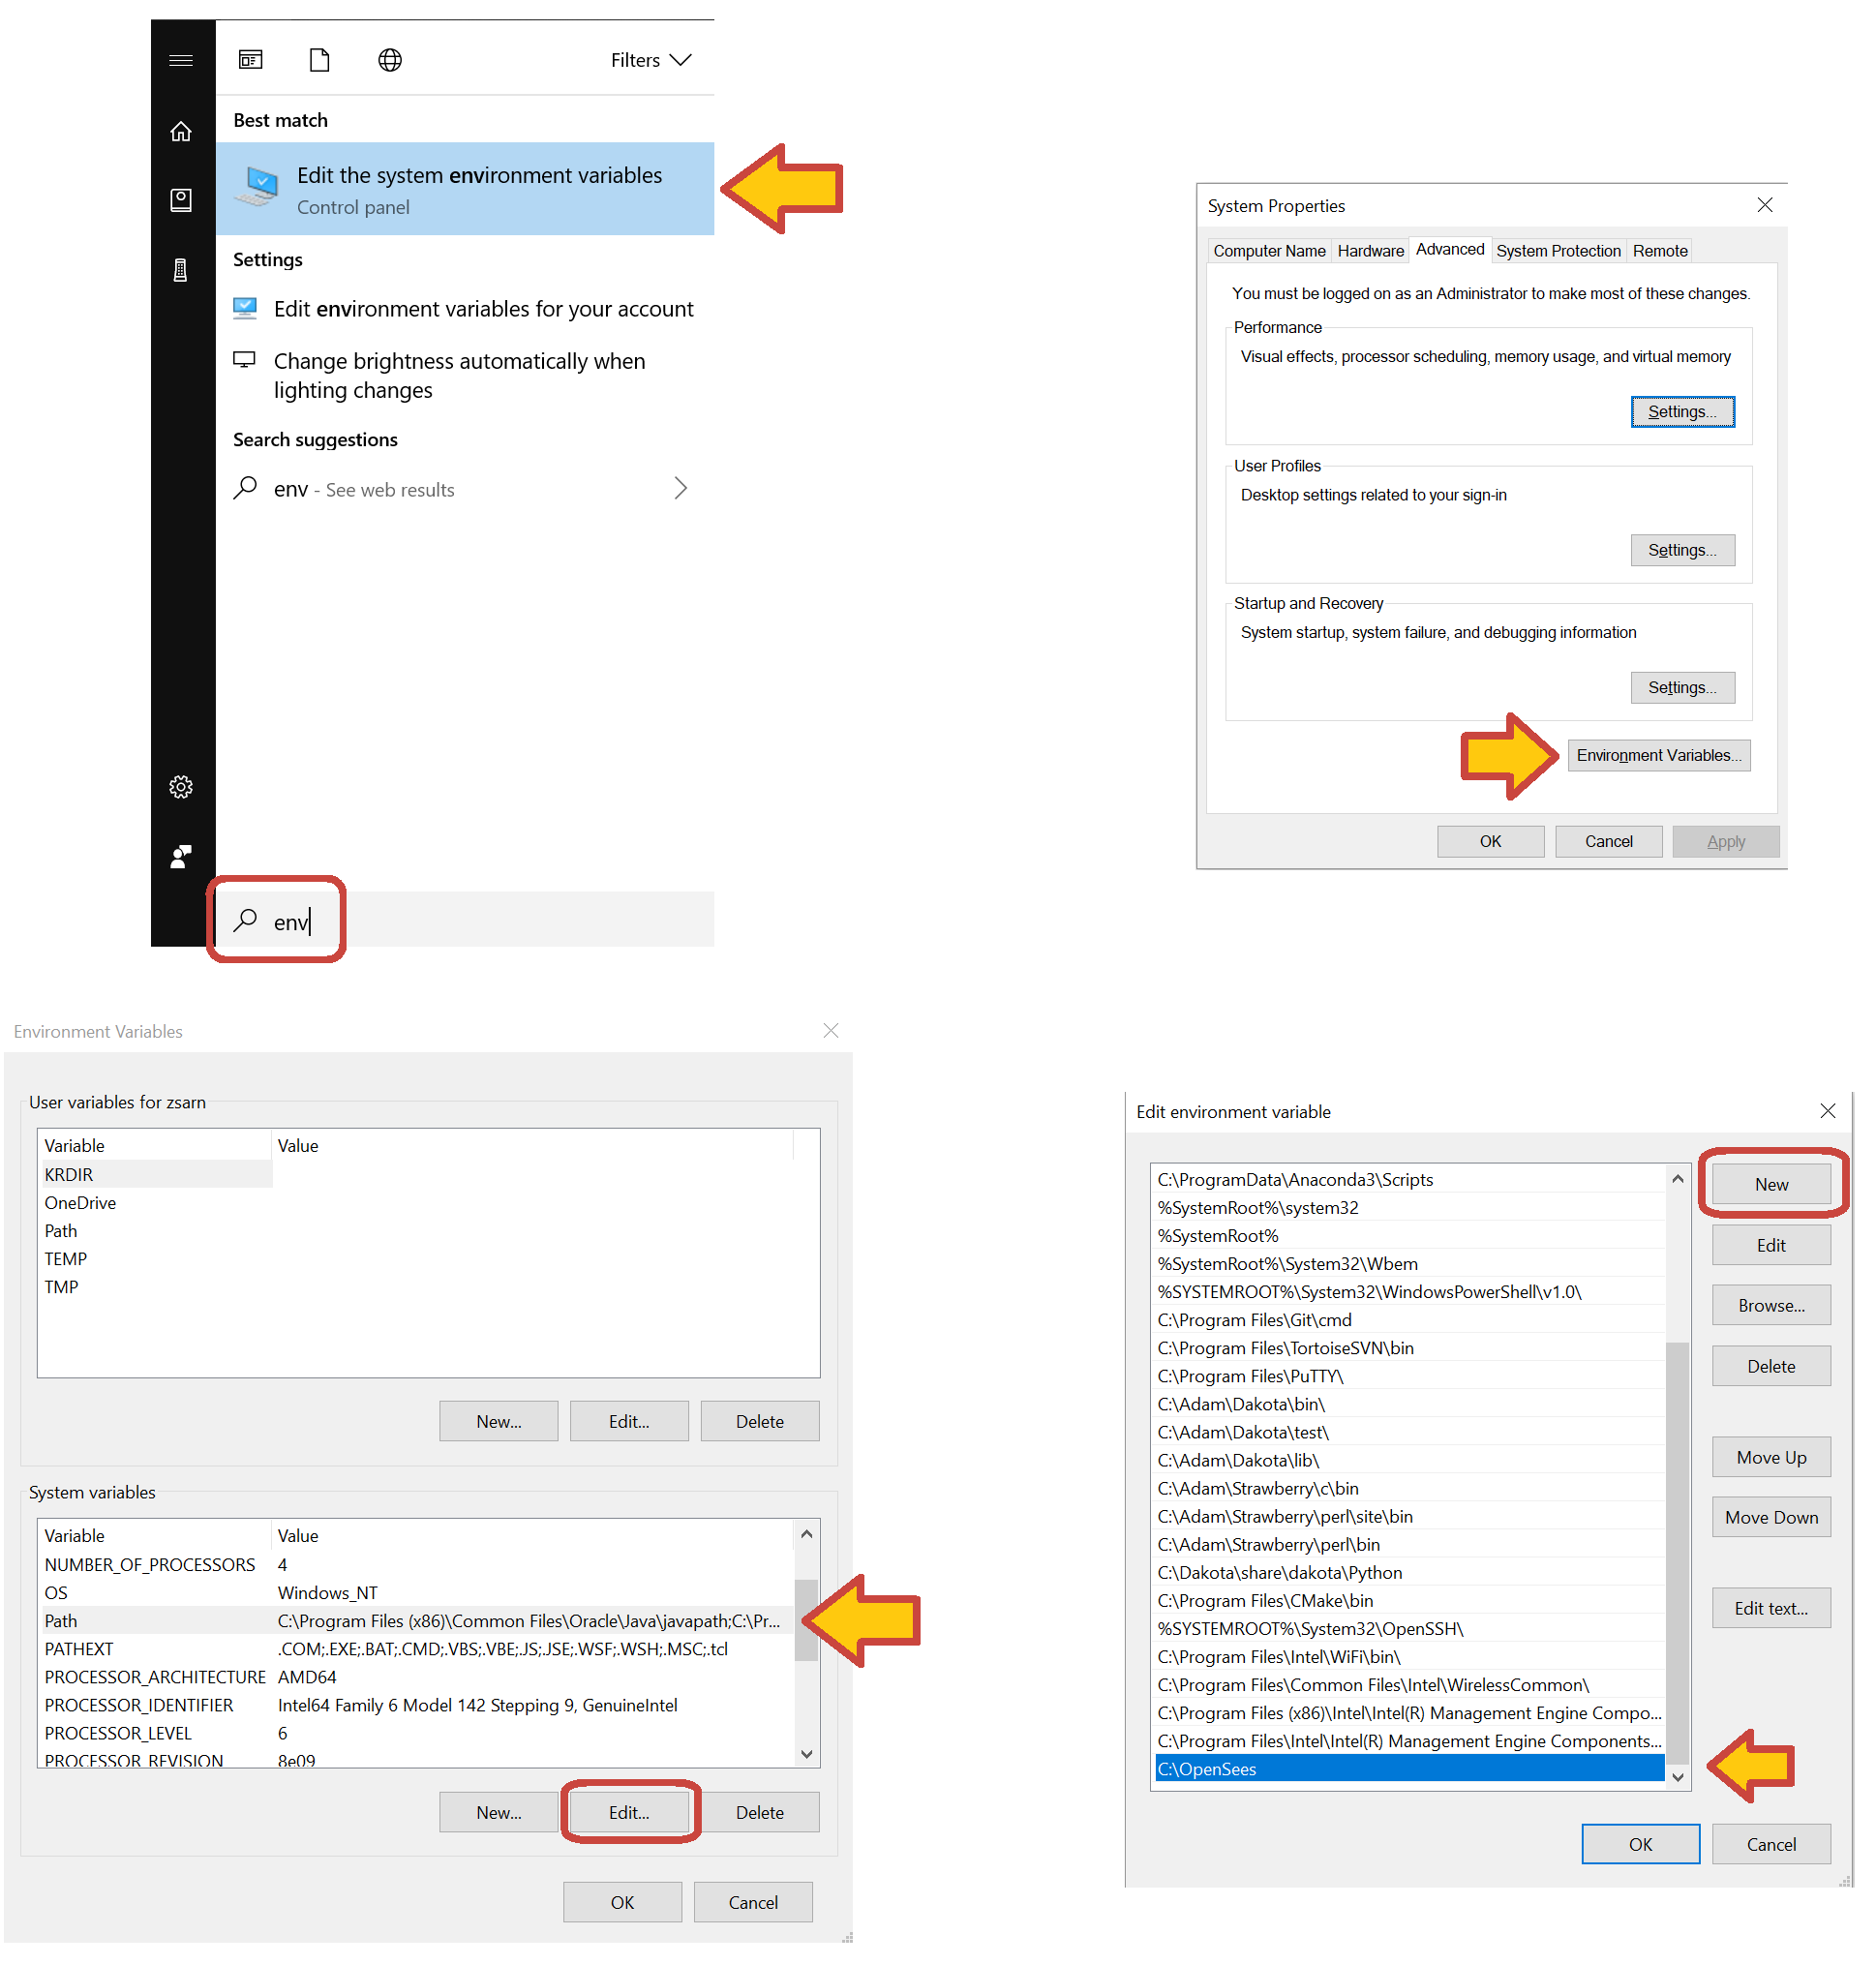
\includegraphics[width=0.8\textwidth]
    {installation/figures/add_env_path.png} }
  \caption{Adding OpenSees to the PATH environment variable on Windows}
  \label{fig:add_env_path}
\end{figure}


\begin{enumerate}
    \item open \emph{Start}, type \emph{env}, and choose \emph{Edit the system environment variables};
    \item click on the \emph{Environment variables...} button in the dialog window;
    \item find the \texttt{Path} under \emph{System Variables} in the \emph{Variable} column;
    \item click \emph{New} and type in the path to your \texttt{OpenSees.exe} (this will be \texttt{C:\textbackslash SimCenter\textbackslash OpenSees} if you put the executable at the recommended location - pay attention to using backslashes here!);
    \item click \emph{OK} in every dialog to close them and save your changes.
\end{enumerate}

\item MacOS: To add the /usr/local/OpenSees folder to the \texttt{PATH} variable:

\begin{enumerate}
    \item open a Terminal;
    \item execute (type the following in the terminal window and hit the return key) the following: \begin{verbatim}nano ${HOME}/.bash_profile\end{verbatim}
    \item if the file contains nothing, add the first 3 lines shown in \Cref{fig:add_env_path_Mac} to the file. This is done in
case an existing .bashrc file exists for your system. Adding these 3 lines will test for the existance of this file, and source in any existing commands if the file does exist.
    \item on a new line add the \texttt{OpenSees} executable to the PATH variable, by typing the following: \begin{verbatim}export PATH=/usr/local/OpenSees:${PATH}\end{verbatim}
    \item quit by hitting \texttt{Ctrl+X} and then \texttt{Y} when asked if you want to save modifications.
    \item test it is entered correctl, the following command now entered in the terminal window should result in no errors: \begin{verbatim}source ${HOME}/.bash_profile\end{verbatim}. 
\end{enumerate}

\begin{figure}[!htbp]
  \centering {
     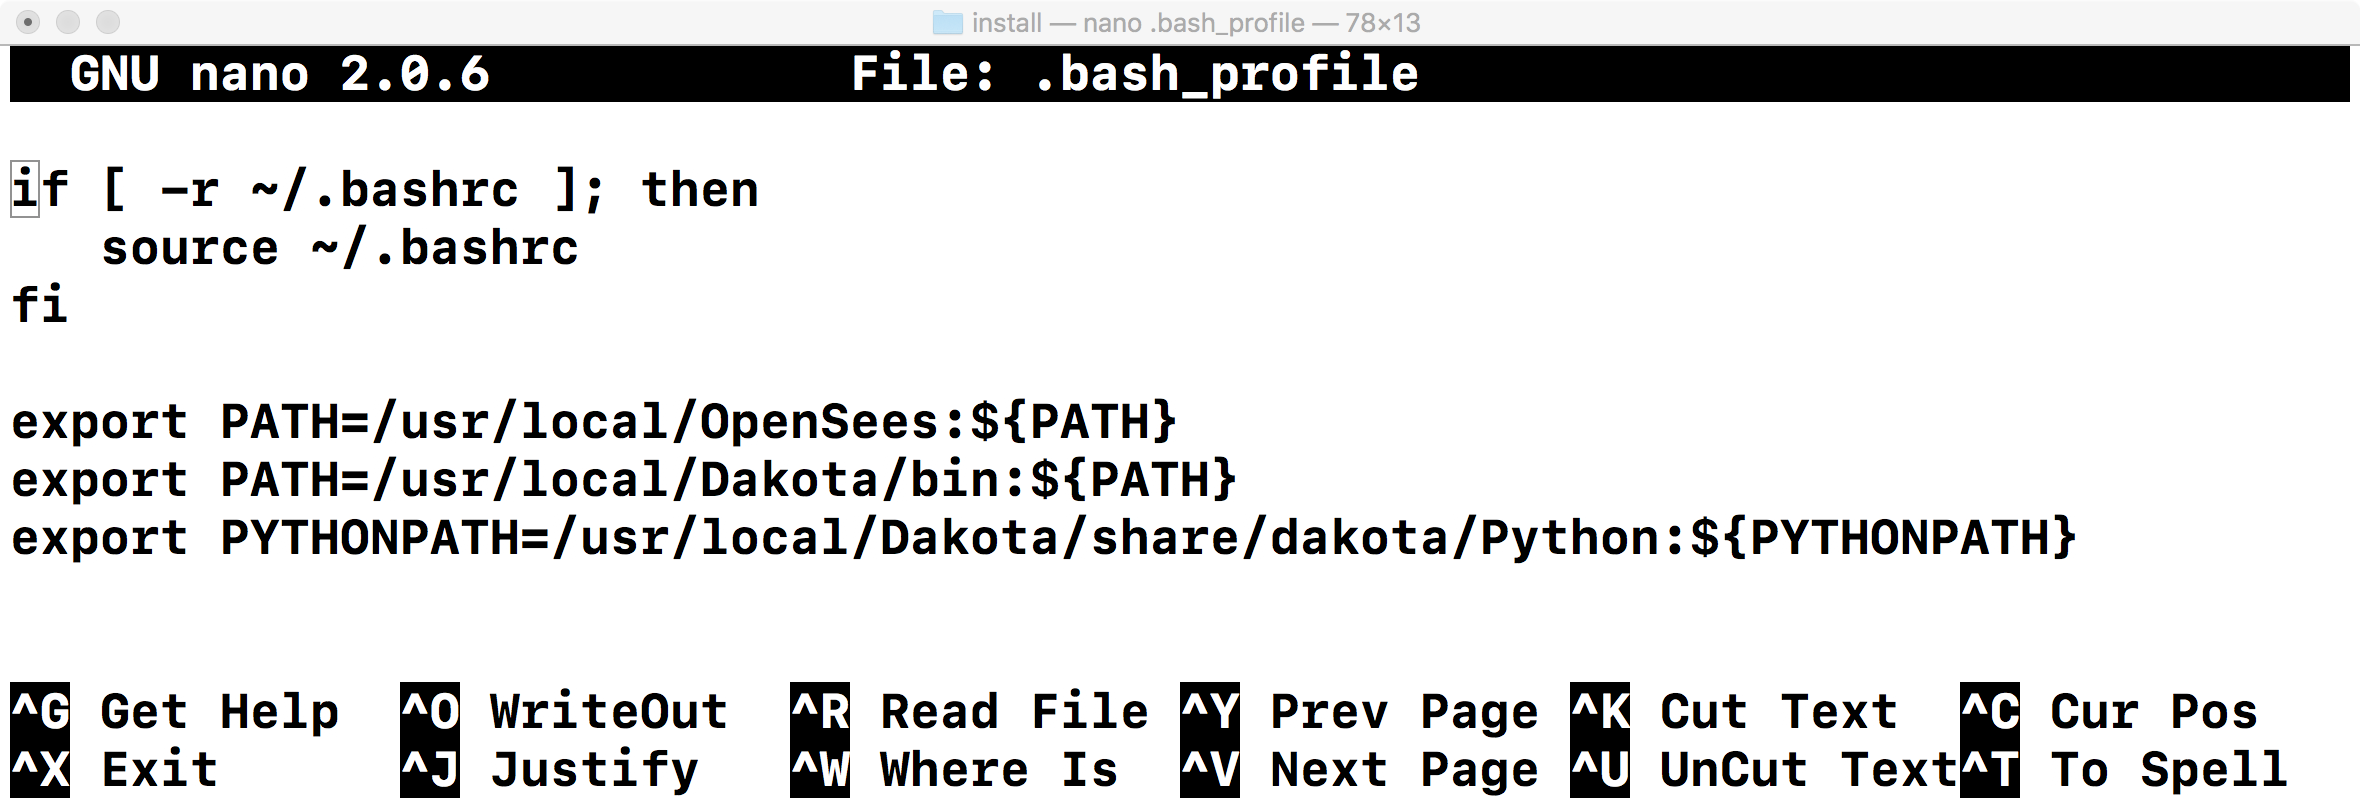
\includegraphics[width=0.8\textwidth]
    {installation/figures/add_env_path_Mac.png} }
  \caption{Adding OpenSees to the PATH environment variable on Mac.}
  \label{fig:add_env_path_Mac}
\end{figure}


\end{enumerate}


\subsection{Install \texttt{Dakota}}
%===============================================================================

\href{http://dakota.sandia.gov}{\texttt{Dakota}}, an open-source  optimization and UQ application from Sandia National Labs, is publicly available for download at its \href{http://dakota.sandia.gov/download.html}{download page}. Select your operating system from the list and set the other options as shown in  \Cref{fig:dakota_installation}. Download the release in a \texttt{ZIP} file for Windows and \texttt{TAR.GZ} file for Mac. We recommend you to extract the archive to a \texttt{C:/SimCenter/Dakota} folder on Windows, and to a \texttt{/usr/local/Dakota} folder on a Mac.

\begin{figure}[!htbp]
  \centering {
    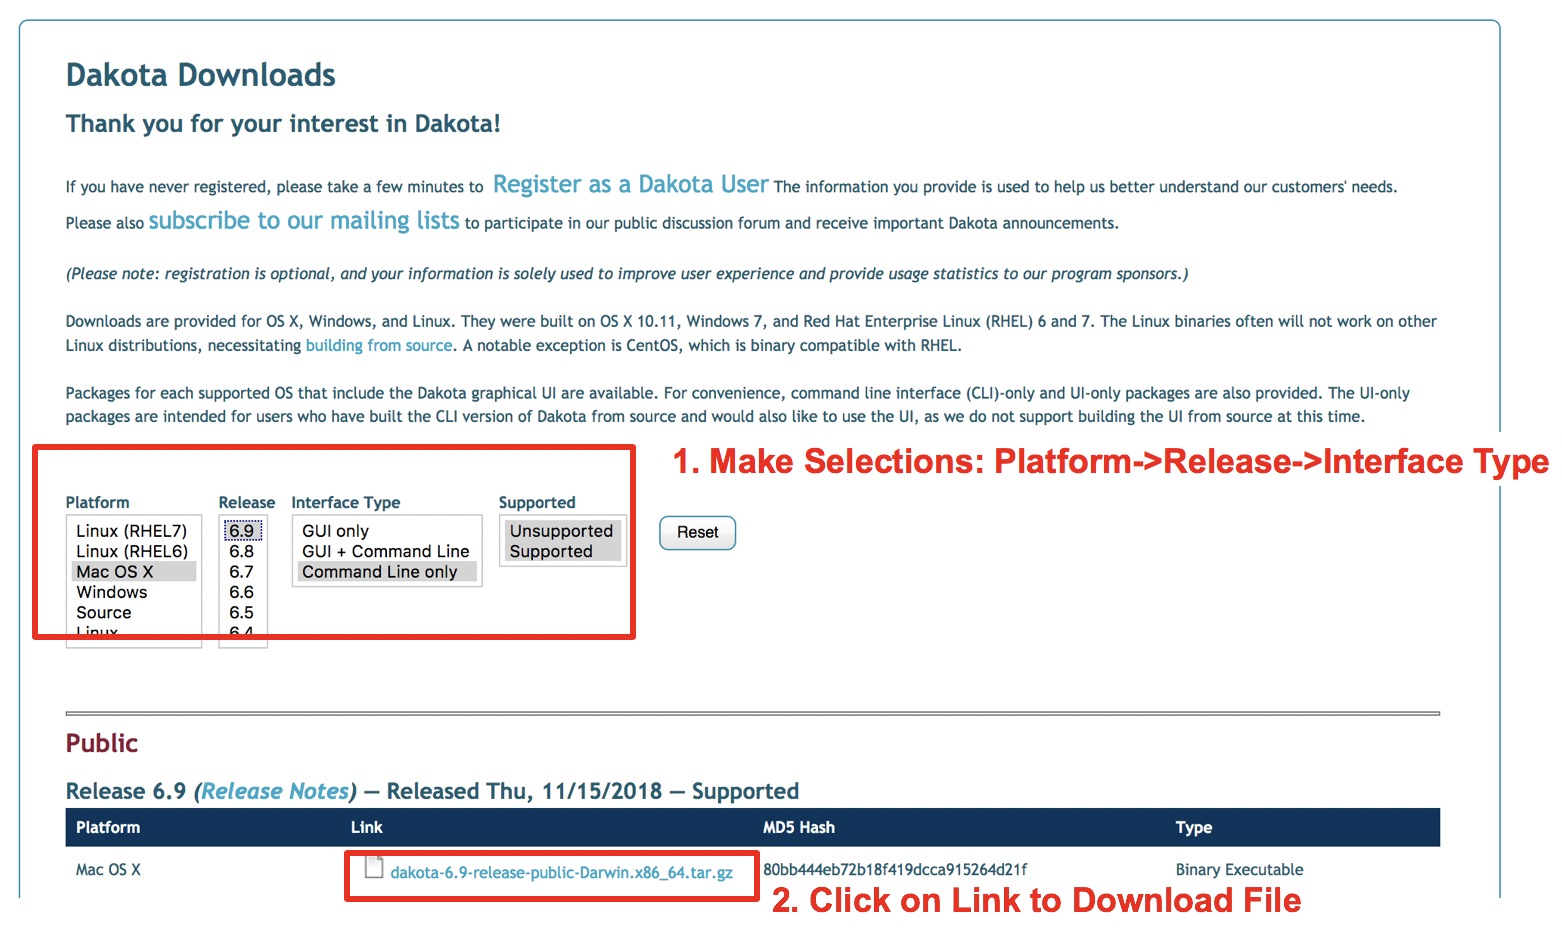
\includegraphics[width=\textwidth]
    {installation/figures/dakota_installation.png} }
  \caption{Downloading Dakota Software}
  \label{fig:dakota_installation}
\end{figure}


Following the instructions provided for installing \texttt{OpenSees}, you need to add \textbf{two} \texttt{Dakota} folders to the system \texttt{PATH} environment variable to allow the SimCenter workflow applications to find the \texttt{Dakota} tools on your computer. 
The procedure described above for \texttt{OpenSees} to add the following
folders to your \texttt{PATH}:

\begin{enumerate}
\item{Windows}

Add the following 2 folders to your windows PATH variable:
\begin{itemize}
    \item \texttt{C:\textbackslash SimCenter\textbackslash Dakota\textbackslash bin}
    \item \texttt{C:\textbackslash SimCenter\textbackslash Dakota\textbackslash share\textbackslash dakota\textbackslash Python}
\end{itemize}

Now you need to create a new variable, \texttt{PYTHONPATH}, and point it to the following folder.


\begin{itemize}
    \item \texttt{C:\textbackslash SimCenter\textbackslash Dakota\textbackslash share\textbackslash dakota\textbackslash Python}
\end{itemize}

\item{MacOS}
On the Mac you also need to add 2 lines, previously shown in \Cref{fig:add_env_path_Mac},
 to the .bash\_profile file. One line adds the Dakota executable to the PATH variablem and 
the other creates a new variable PYTHONPATH and points it to a folder in the  Dakota 
installation directory. 

\begin{itemize}
    \item \texttt{export PATH=/usr/local/Dakota/bin:\${PATH}}
    \item \texttt{export PYTHONPATH=/usr/local/Dakota/share/dakota/Python}
\end{itemize}
\end{enumerate}

NOTE: Apple, in the latest release of their operating system, MacOS 10.16 Catalina, has changed the default working of Gatekeeper.
Gatekeeper, first introduced in OS X Mountain Lion, is a Mac security feature that helps protect your Mac from Malware and other malicious software. Gatekeeper checks to make sure the application is safe to run by checking it against the list of apps that Apple has vetted and approved for the Apple Mac Store and/or approved by Apple even if not offered through the app store. In previous versions of MacOS, Gatekeeper had three security level options: App Store, App Store and Identified Developers, and Anywhere. Anywhere has been removed and this will cause problems with Dakota. As a consequence, it is necessary to follow the following when you update the MacOS or install Dakota for the first time on machine with an updated MacOS. From the terminal app, with the above .bash\_profile settings set, you need to type the following in the terminal window:

\begin{verbatim}
sudo spctl --master-disable
dakota
sudo spctl --master-enable
\end{verbatim}

This will temporarily disable gatekeeper (basically setting Gatekeeper options to Anywhere), allow the Dakota application and it's .dylib files to be registered as safe, and then turn Gatekeeper options back to default.


\subsection{Install  Perl}
%===============================================================================

Mac OS X has Perl pre-installed, but Windows users will have to
install it to be able to use \texttt{Dakota}. We recommend you use Strawberry
Perl; you can install it by downloading the executable from
its \href{http://strawberryperl.com}{Strawberry Perl website} and
running it.

\subsection{Test the Install of the Local Applications}
%===============================================================================

Before running the \texttt{\getsoftwarename{}} application, perform the following tests to
make sure that the local SimCenter working environment is set up
appropriately:

\begin{itemize}
    \item Start a Terminal on Mac or a Command Prompt on Windows.
    \item On Mac, execute \texttt{cd /usr/Documents} to change the active directory to \texttt{/usr/Documents}. On Windows, execute \texttt{cd C:/} to change the active directory to \texttt{C:/}.
    \item Test if \texttt{OpenSees} works correctly by executing the \texttt{OpenSees} command. The command should start \texttt{OpenSees} (\Cref{fig:opensees_test}). Close \texttt{OpenSees} with the \texttt{exit} command.
    \item Test if \texttt{Dakota} works correctly by executing the \texttt{dakota} command. The command should start \texttt{Dakota} and you should see a message about a missing argument (\Cref{fig:dakota_test}).
    \item Test if Perl works correctly by executing the \texttt{perl -v} command. The command should start Perl and return its version number (\Cref{fig:perl_test}).
    \item Test if the python package in \texttt{Dakota} works correctly by starting Python with the \texttt{python} command and then executing the \texttt{import dakota} command. This should import the dakota package. If you do not see errors, then the package is successfully imported (\Cref{fig:dakota_py_test}). Exit Python with the \texttt{exit()} command.
    \item If all the above tests ran without errors, your environment is set up appropriately.
\end{itemize}

\begin{figure}[!htbp]
  \centering {
    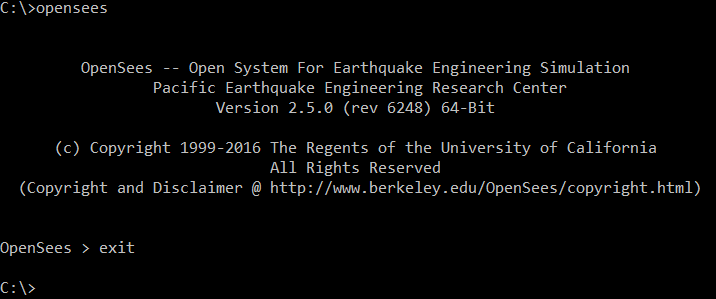
\includegraphics[width=0.8\textwidth]
    {installation/figures/opensees_test.png} }
  \caption{Testing OpenSees.}
  \label{fig:opensees_test}
\end{figure}

\begin{figure}[!htbp]
  \centering {
    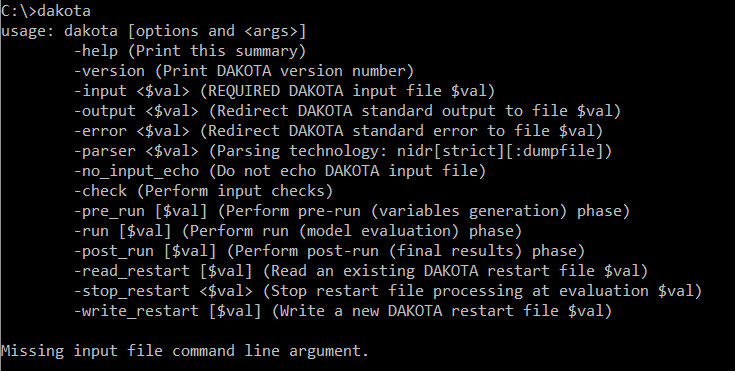
\includegraphics[width=0.8\textwidth]
    {installation/figures/dakota_test.png} }
  \caption{Testing Dakota.}
  \label{fig:dakota_test}
\end{figure}

\begin{figure}[!htbp]
  \centering {
    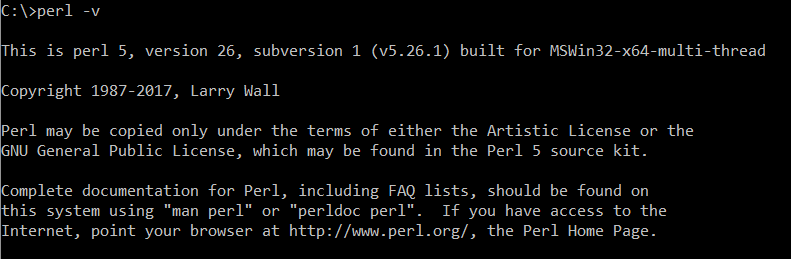
\includegraphics[width=0.8\textwidth]
    {installation/figures/perl_test.png} }
  \caption{Testing Perl.}
  \label{fig:perl_test}
\end{figure}

\begin{figure}[!htbp]
  \centering {
    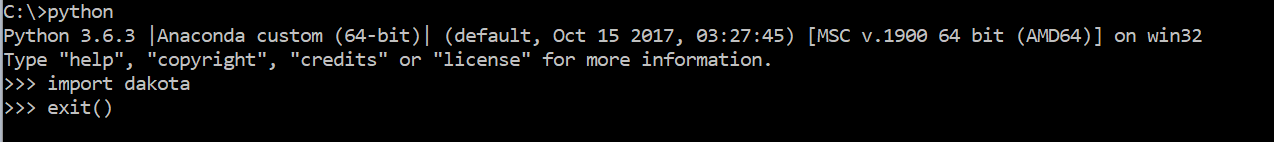
\includegraphics[width=0.8\textwidth]
    {installation/figures/dakota_py_test.png} }
  \caption{Testing the dakota Python package.}
  \label{fig:dakota_py_test}
\end{figure}

%===============================================================================
\clearpage
\section{Test the \texttt{\getsoftwarename{}} application}
\label{sec:test_local}


\softwareSwitch{WE-UQ}{
Once the local SimCenter working environment has been tested and is
functioning correctly, the \texttt{\getsoftwarename{}} Application
can be tested. The simplest way to do this is by running an analysis
using the default structural model with synthetic wind event. By
doing this, it is not necessary to enter any information on the
structural model and only inputs for the synthetic wind forces 
and uncertainty quantification are required. With this quick setup, the
functionality of the \texttt{\getsoftwarename{}} UI and the associated backend
workflow can be tested. The necessary steps to perform this
testing are provided below.

A full description of how to use this software is provided
in \Cref{chap:usage}.  In this quick test, users will only
interface with the event tab (\texttt{EVT}), the uncertainty
quantification tab (\texttt{UQ}), and the results tab (\texttt{RES}).

The first step is to start the \texttt{\getsoftwarename{}}
<<<<<<< HEAD
application. Click on the \texttt{EVT} tab which will allow 
the loading type to be selected. From the dropdown menu select 
\texttt{Stochastic Wind}. The model will be set as 
\texttt{Wittag and Sinha (1975)} as shown in \Cref{fig:input_event}.
=======
application.  Once the application is started, the second step is to
input the parameters for the synthetic motions under the \texttt{EVT}
(Event) tab. This is shown in \Cref{fig:input_event}. Click
on the \texttt{EVT} tab which will allow the loading type to be
selected. From the dropdown menu select \texttt{Stochastic Wind Event}
model will be set as \texttt{Wittag and Sinha (1975)}.
>>>>>>> upstream/master

\begin{figure}[!htbp]
  \centering {
    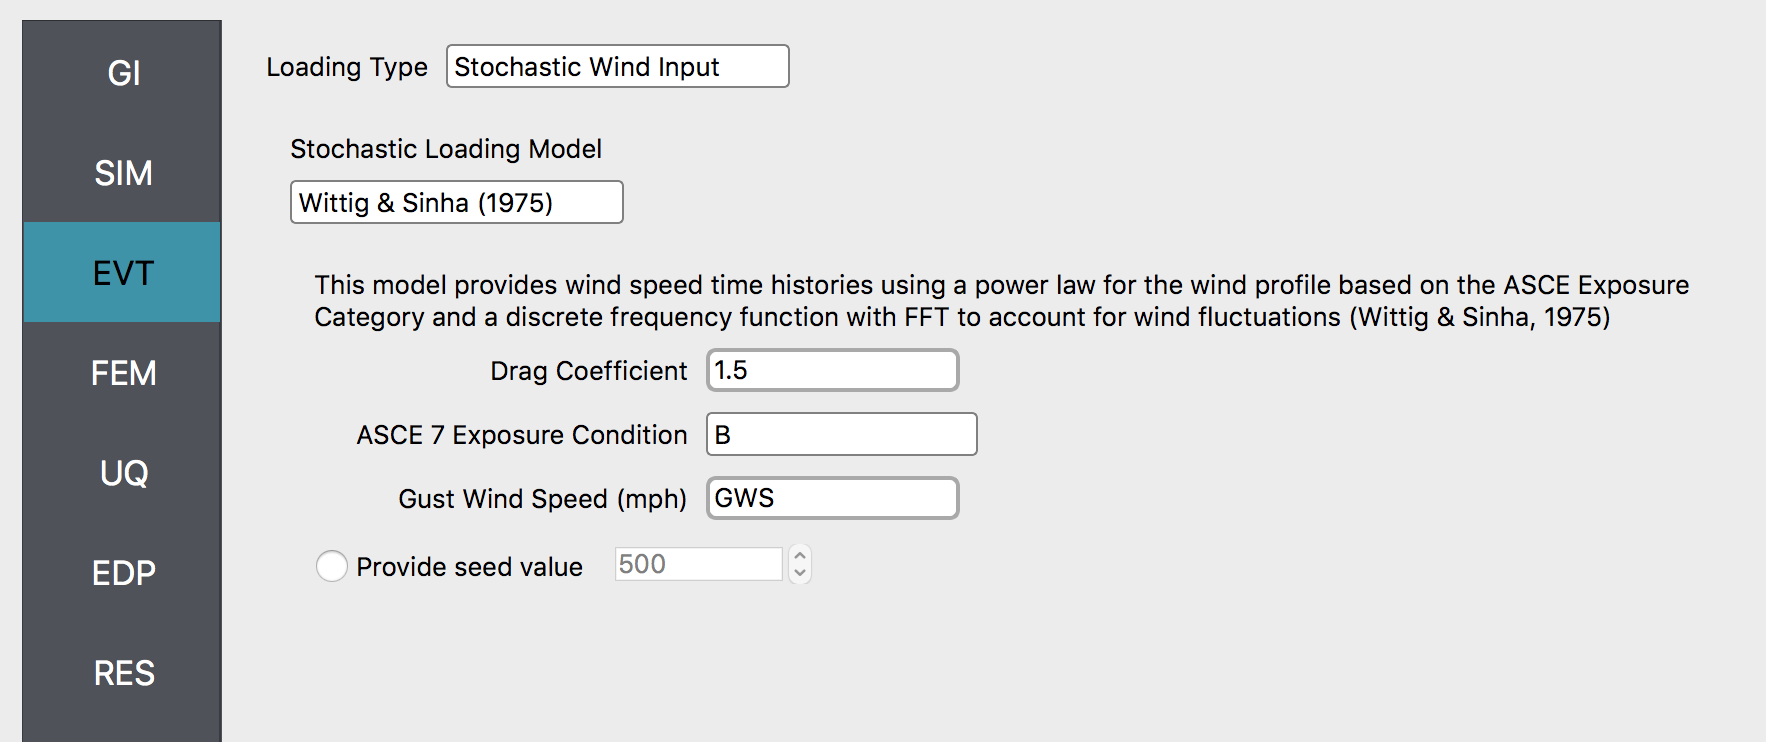
\includegraphics[width=0.7\textwidth]
    {installation/figures/testWE_EVT.png} }
  \caption{Selecting event type and inputting synthetic motion parameters}
  \label{fig:input_event}
\end{figure}

Only three inputs are required for this test, of which one will be set
to a random variable. As shown in \Cref{fig:input_event}, set the
\emph{Drag Coefficient} to {\texttt 1.5}, \emph{exposure condition} to \texttt{B}, and \emph{Gust Wind Speed} to \texttt{GWS}.
to \texttt{vs30}. The \texttt{Provide seed value} radio button should
<<<<<<< HEAD
be left unselected. By specifying these inputs, both drag coefficient and the
exposure condition will have constant values in all realizations while \texttt{GWS} will have different values based on the model parameters specified in the
uncertainty quantification (\texttt{UQ}) tab. With these inputs specified, click on the \texttt{UQ} tab. Here the distributions and their relevant parameters will be specified for the random variables defined in the analysis\textemdash only $GWS$
in this case. Since $GWS$ was identified as a random variable
by inputting the parameter value as text, it is automatically added as
a random variable, as shown in \Cref{fig:input_uq}. Set the
distribution type to \texttt{normal} with a \texttt{Mean}
and \texttt{Standard Dev} of 100 and 10 mph,
=======
be left unselected. By specifying these inputs, both drag coefficient
and the exposure condition will have constant values in all
realizations while \texttt{GWS} will have different values based on
the model parameters specified in the uncertainty quantification
(\texttt{UQ}) tab. With these inputs specified, navigate to
the \texttt{UQ} tab. Here the distributions and their relevant
parameters will be specified for the random variables defined in the
analysis\textemdash only $GWS$ in this case. Since $GWS$ was
identified as a random variable by inputting the parameter value as
text, it is automatically added as a random variable, as shown
in \Cref{fig:input_uq}. Set the distribution type to \texttt{normal}
with a \texttt{Mean} and \texttt{Standard Dev} of 100 and 10 mph,
>>>>>>> upstream/master
respectively.

\begin{figure}[!htbp]
  \centering {
    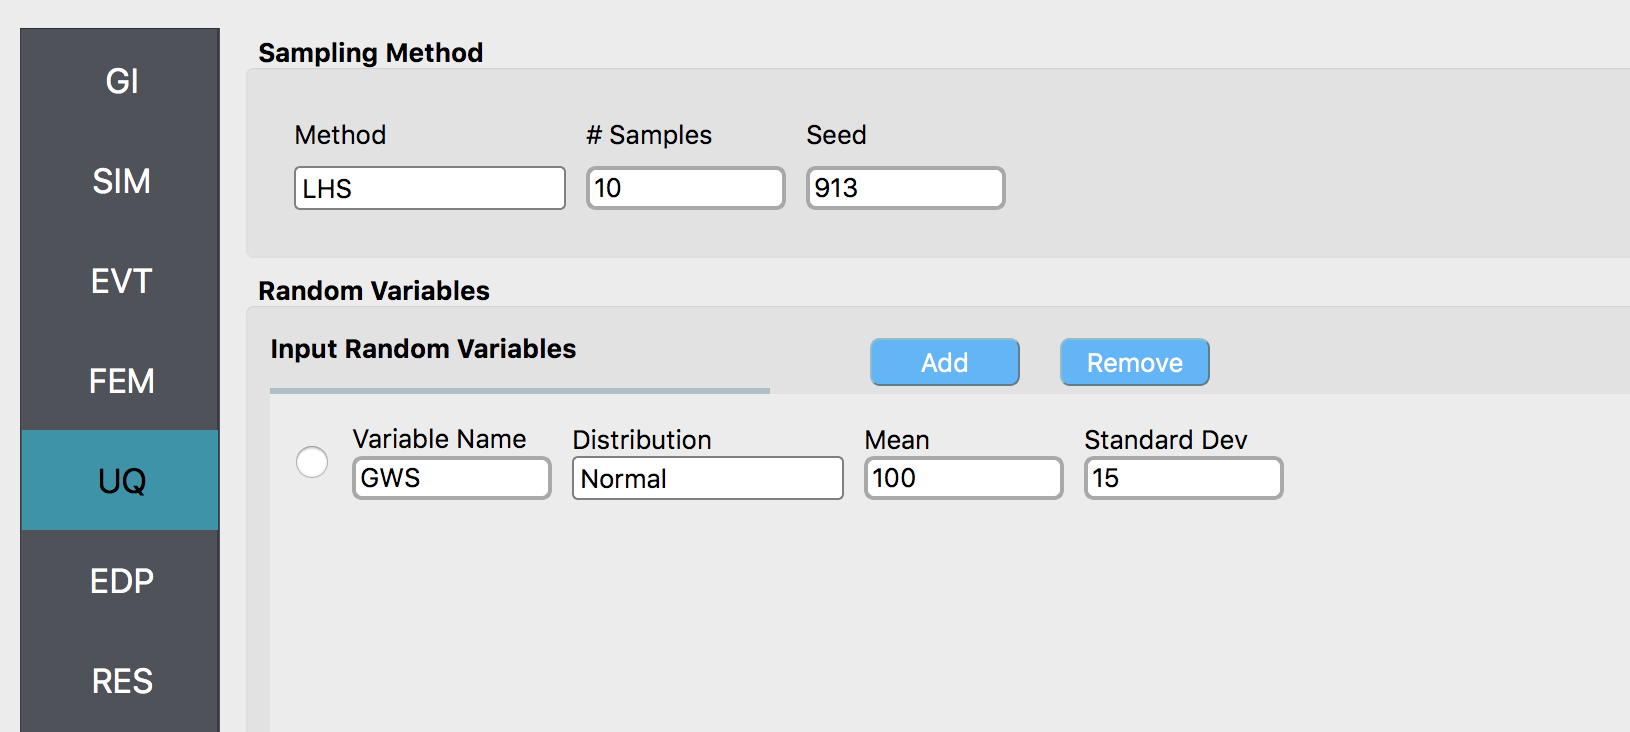
\includegraphics[width=0.7\textwidth]
    {installation/figures/testWE_UQ.png} }
  \caption{Specifying distribution type and parameters for random
  variables in analysis\textemdash only $GWS$ in this case}
  \label{fig:input_uq}
\end{figure}

Now, click on the \texttt{RUN} button, which will bring up a pop-up
menu that provides information on the application directory and
the working directory. The application directory should already be
automatically set to where \texttt{\getsoftwarename{}} is installed.
If desired, the working directory can be changed. In order to start
the analysis, click on the \texttt{Submit} button.

\begin{figure}[!htbp]
  \centering {
    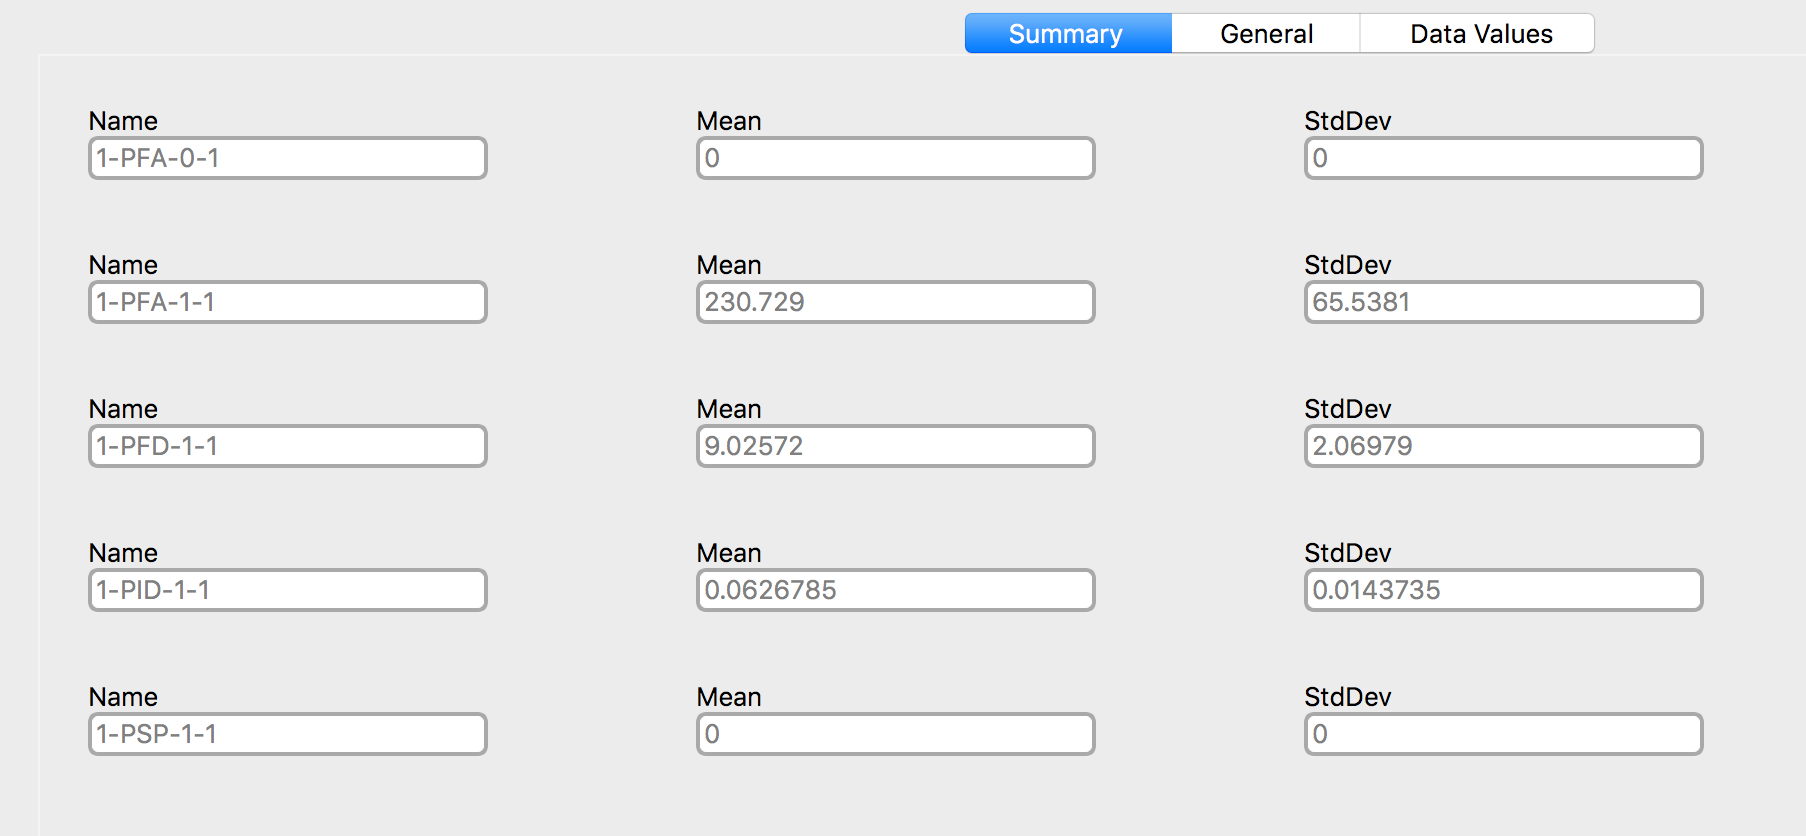
\includegraphics[width=0.7\textwidth]
    {installation/figures/testWE_RES.png} }
  \caption{Results for test analysis. This tab will open automatically
  when the analysis completes, indicating a successful installation}
  \label{fig:show_results}
\end{figure}



If successful, the application will pause briefly while it runs the
analysis before automatically displaying the simulations results in
the \texttt{RES} tab, as shown
in \Cref{fig:show_results}. Remember, the results shown
in \Cref{fig:show_results} most likely will not be the same as
those from this local test since $GWS$ is a random variable and
the values realized in the simulations will be different while still
following the same distribution. In any case, if the simulations
completed and the \texttt{RES} tab is showing simulation results, then
the \texttt{\getsoftwarename{}} App is properly installed and configured.

}{
Once the local SimCenter working environment has been tested and is
functioning correctly, the \texttt{\getsoftwarename{}} Application
can be tested. The simplest way to do this is by running an analysis
using the default structural model with synthetic ground motions. By
doing this, it is not necessary to enter any information on the
structural model and only inputs for
\softwareSwitch{WE-UQ}{
the synthetic wind forces and uncertainty quantification
}{}
\softwareSwitch{EE-UQ}{
the synthetic motions and uncertainty quantification
}{}
\softwareSwitch{PBE}{
the synthetic motions, uncertainty quantification, and loss assessment
}{}
are required. With this quick setup, the
functionality of the \texttt{\getsoftwarename{}} UI and the associated backend
workflow can be tested. The steps to perform this
testing are provided below.

A full description of how to use this software is provided
in \Cref{chap:usage}.  In this quick test, users will only
interface with the event tab (\texttt{EVT}), the uncertainty
quantification tab (\texttt{UQ}), 
\softwareSwitch{PBE}{
the damage and loss assessment tab (\texttt{DL}),
}{}
and the results tab (\texttt{RES}).

The first step is to start the \texttt{\getsoftwarename{}}
application.  Once the application is started, the second step is to
input the parameters for the synthetic motions under the \texttt{EVT}
(Event) tab. This is shown in \Cref{fig:input_event}. Click
on the \texttt{EVT} tab which will allow the loading type to be
selected. From the dropdown menu select 
\softwareSwitch{WE-UQ}{
\texttt{Stochastic Wind Event}. 
}{
\texttt{Stochastic Ground Motion Model}. Upon selecting this loading type, the loading 
model will be set as \texttt{Vlachos et al. (2018)}.
}


\softwareSwitch{PBE}{
\begin{figure}[!htbp]
  \centering {
    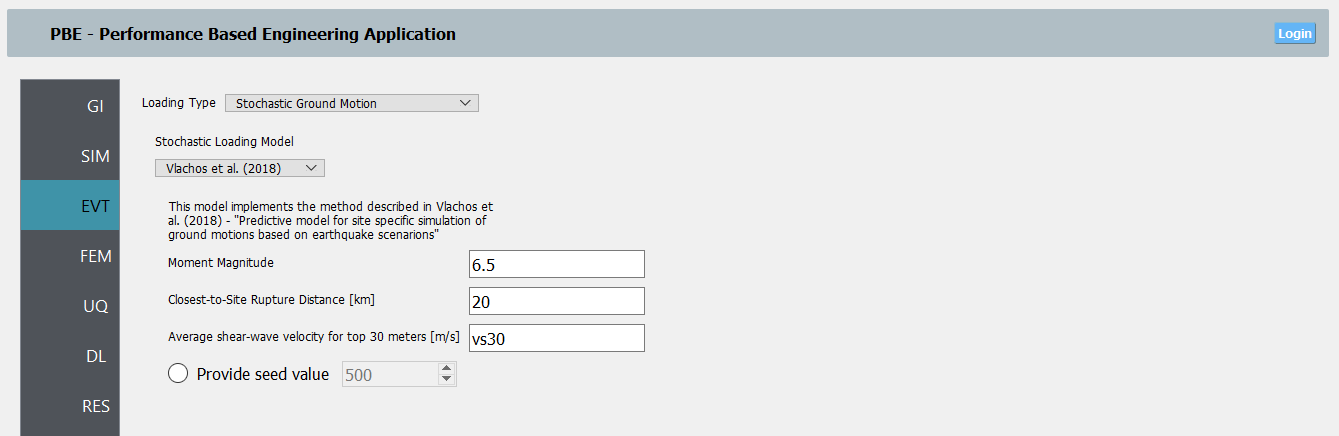
\includegraphics[width=0.95\textwidth]
    {installation/figures/test_input_event_pbe.png} }
  \caption{Selecting event type and inputting synthetic motion parameters}
  \label{fig:input_event}
\end{figure}
}{}
\softwareSwitch{EE-UQ}{
\begin{figure}[!htbp]
  \centering {
    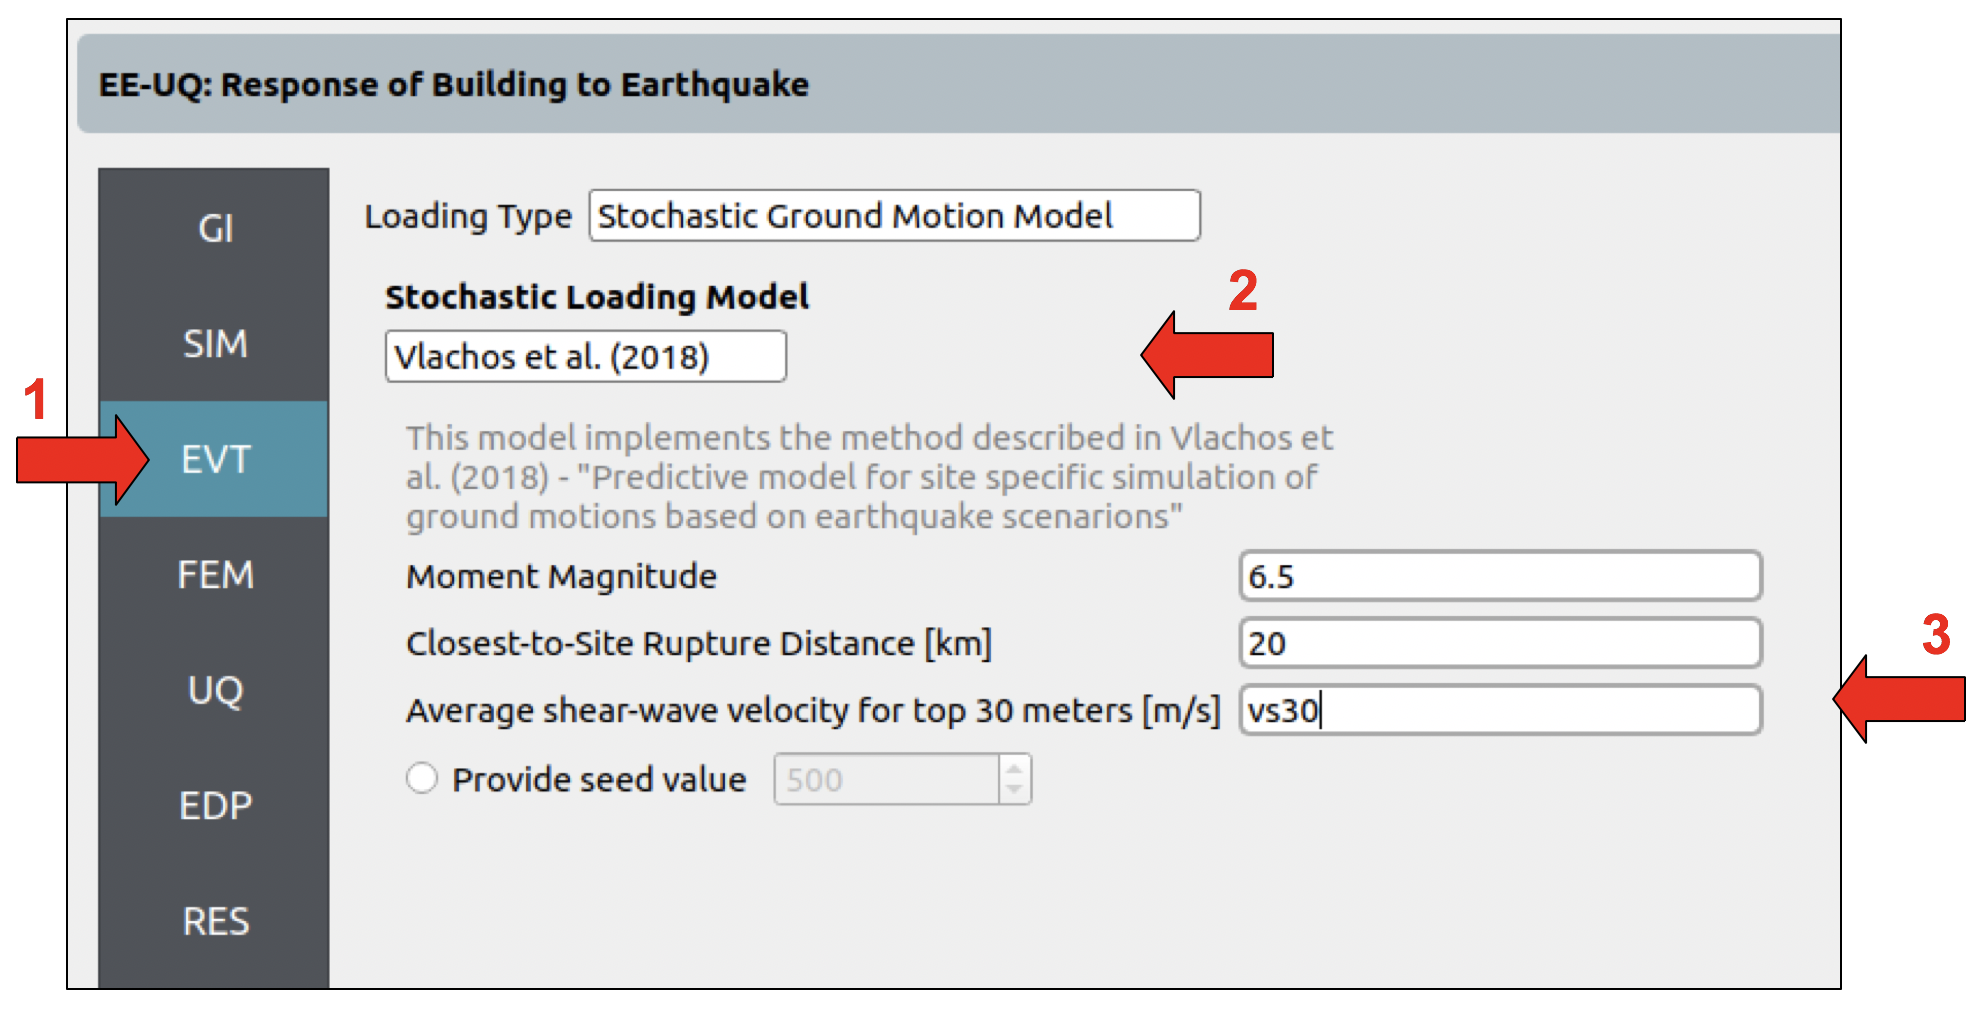
\includegraphics[width=0.7\textwidth]
    {installation/figures/test_input_event.png} }
  \caption{Selecting event type and inputting synthetic motion parameters}
  \label{fig:input_event}
\end{figure}
}{}
\softwareSwitch{WE-UQ}{
\begin{figure}[!htbp]
  \centering {
    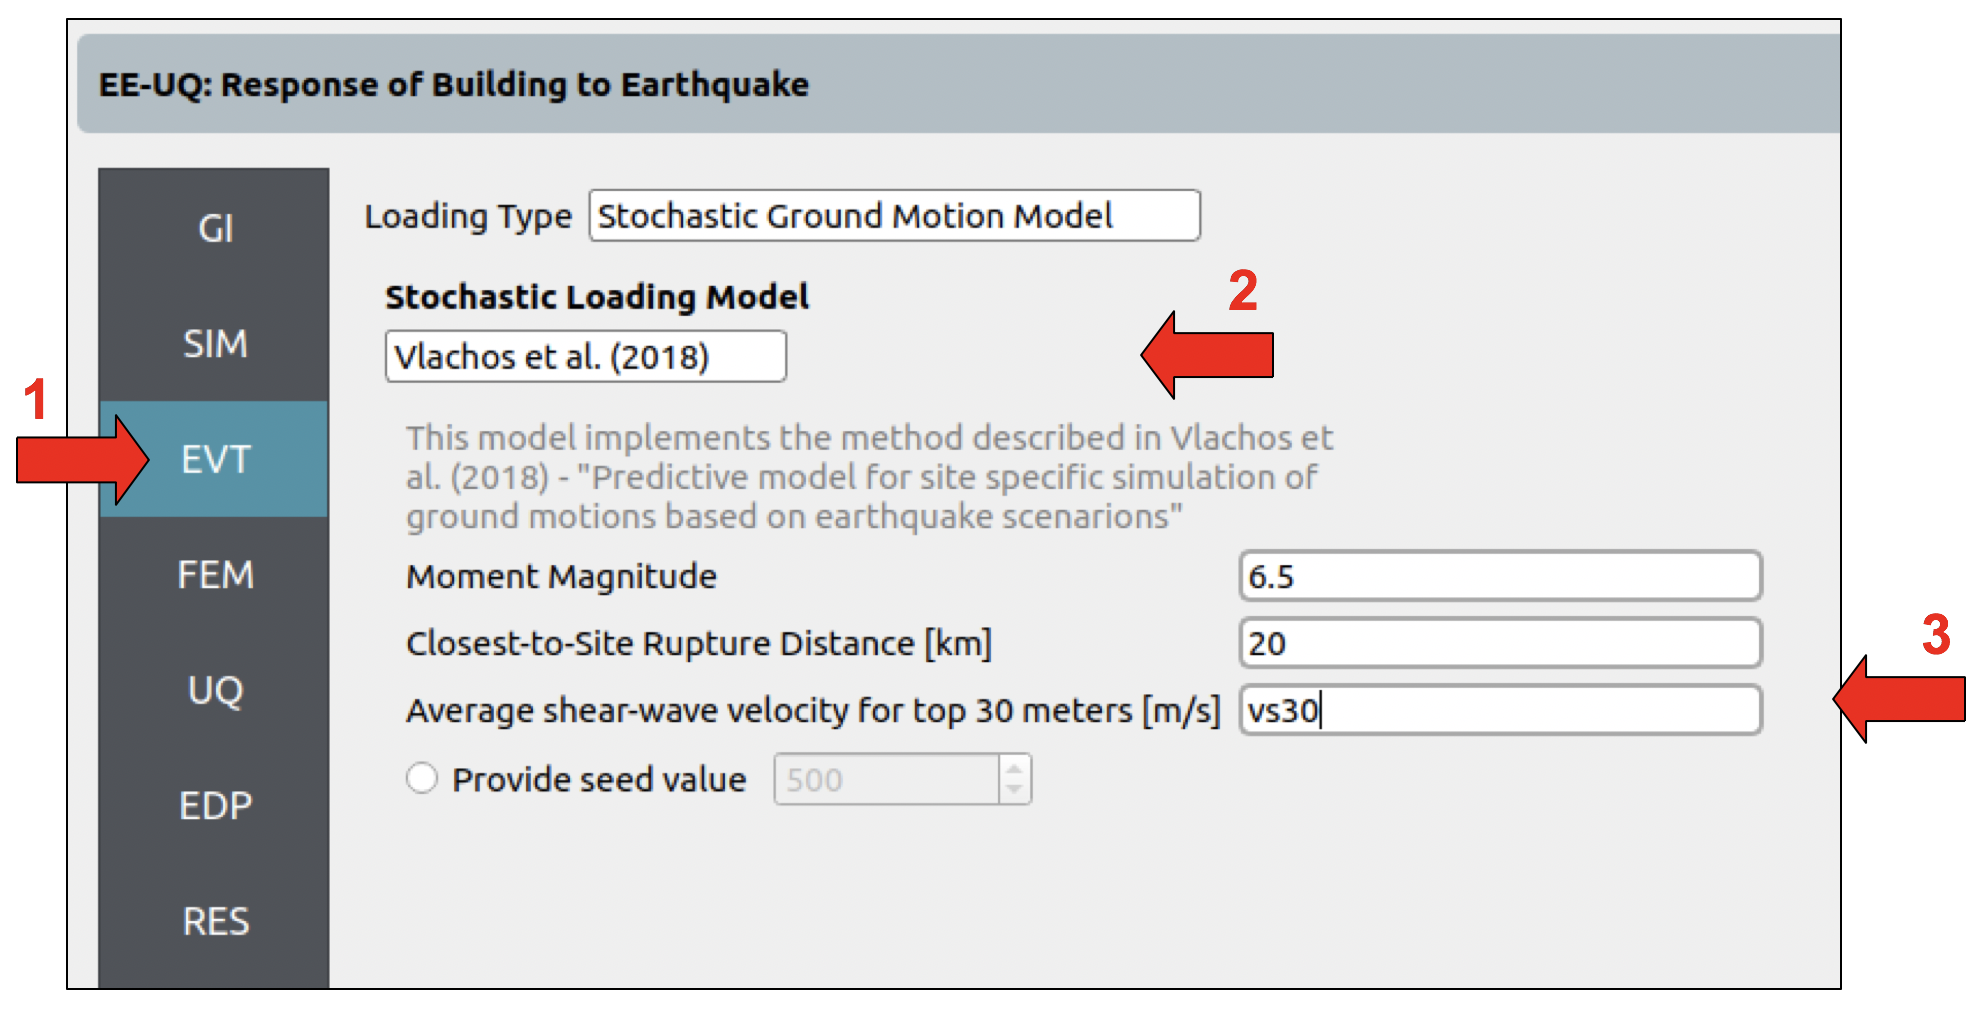
\includegraphics[width=0.7\textwidth]
    {installation/figures/test_input_event.png} }
  \caption{Selecting event type and inputting event parameters}
  \label{fig:input_event}
\end{figure}
}{}

\softwareSwitch{WE-UQ}{
FMK SOME TEXT NEEDED
}{
Only three inputs are required for this test, of which one will be set
to a random variable. As shown in \Cref{fig:input_event}, set the
\emph{Moment Magnitude} ($M_W$) to 6.5, the \emph{Closest-to-Site Rupture Distance}
($R_{rupt}$) to 20 km, and the \emph{Average shear-wave velocity
for the top 30 m} ($V_{S_{30}}$)
to \texttt{vs30}. The \texttt{Provide seed value} radio button should
be left unselected. By specifying these inputs, both $M_{W}$ and $R_{rupt}$
will have constant values in all realizations while $V_{S_{30}}$ will
have different values based on the model parameters specified in the
uncertainty quantification (\texttt{UQ}) tab. With these inputs specified, navigate to the \texttt{UQ} tab. Once in the \texttt{UQ} tab, start with setting the number of samples (\# Samples under \emph{Sampling Method}) to 10. Next, the distributions and their relevant parameters will be specified for the random variables defined in the analysis\textemdash only $V_{S_{30}}$ in this case. Since $V_{S_{30}}$ was identified as a random variable
by inputting the parameter value as text, it is automatically added as a random variable, as shown in \Cref{fig:input_uq}. Set the distribution type to \texttt{normal} with a \texttt{Mean} and \texttt{Standard Dev} of 350 m/s and 25 m/s, respectively.
}

\softwareSwitch{PBE}{
\begin{figure}[!htbp]
  \centering {
    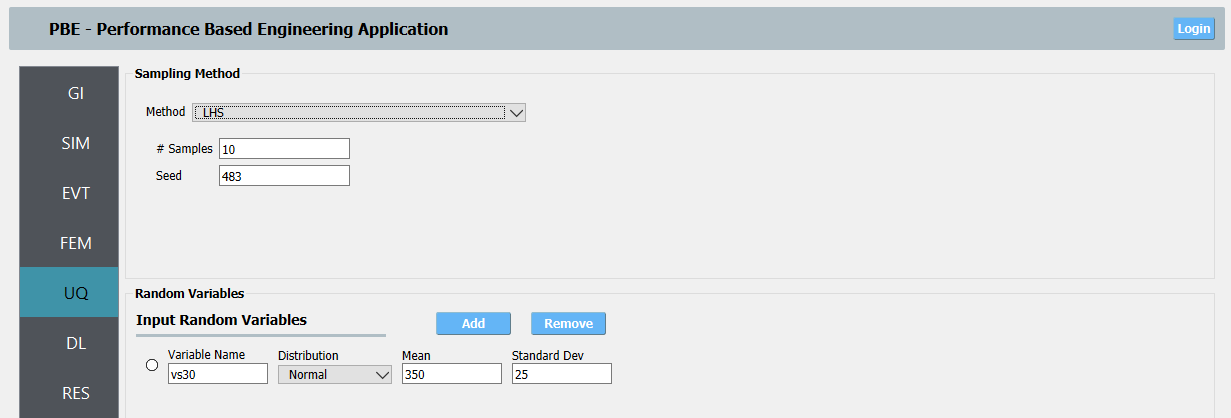
\includegraphics[width=0.95\textwidth]
    {installation/figures/test_input_uq_pbe.png} }
  \caption{Specifying distribution type and parameters for random
  variables in analysis\textemdash only $V_{s30}$ in this case}
  \label{fig:input_uq}
\end{figure}
}{}
\softwareSwitch{EE-UQ}{
\begin{figure}[!htbp]
  \centering {
    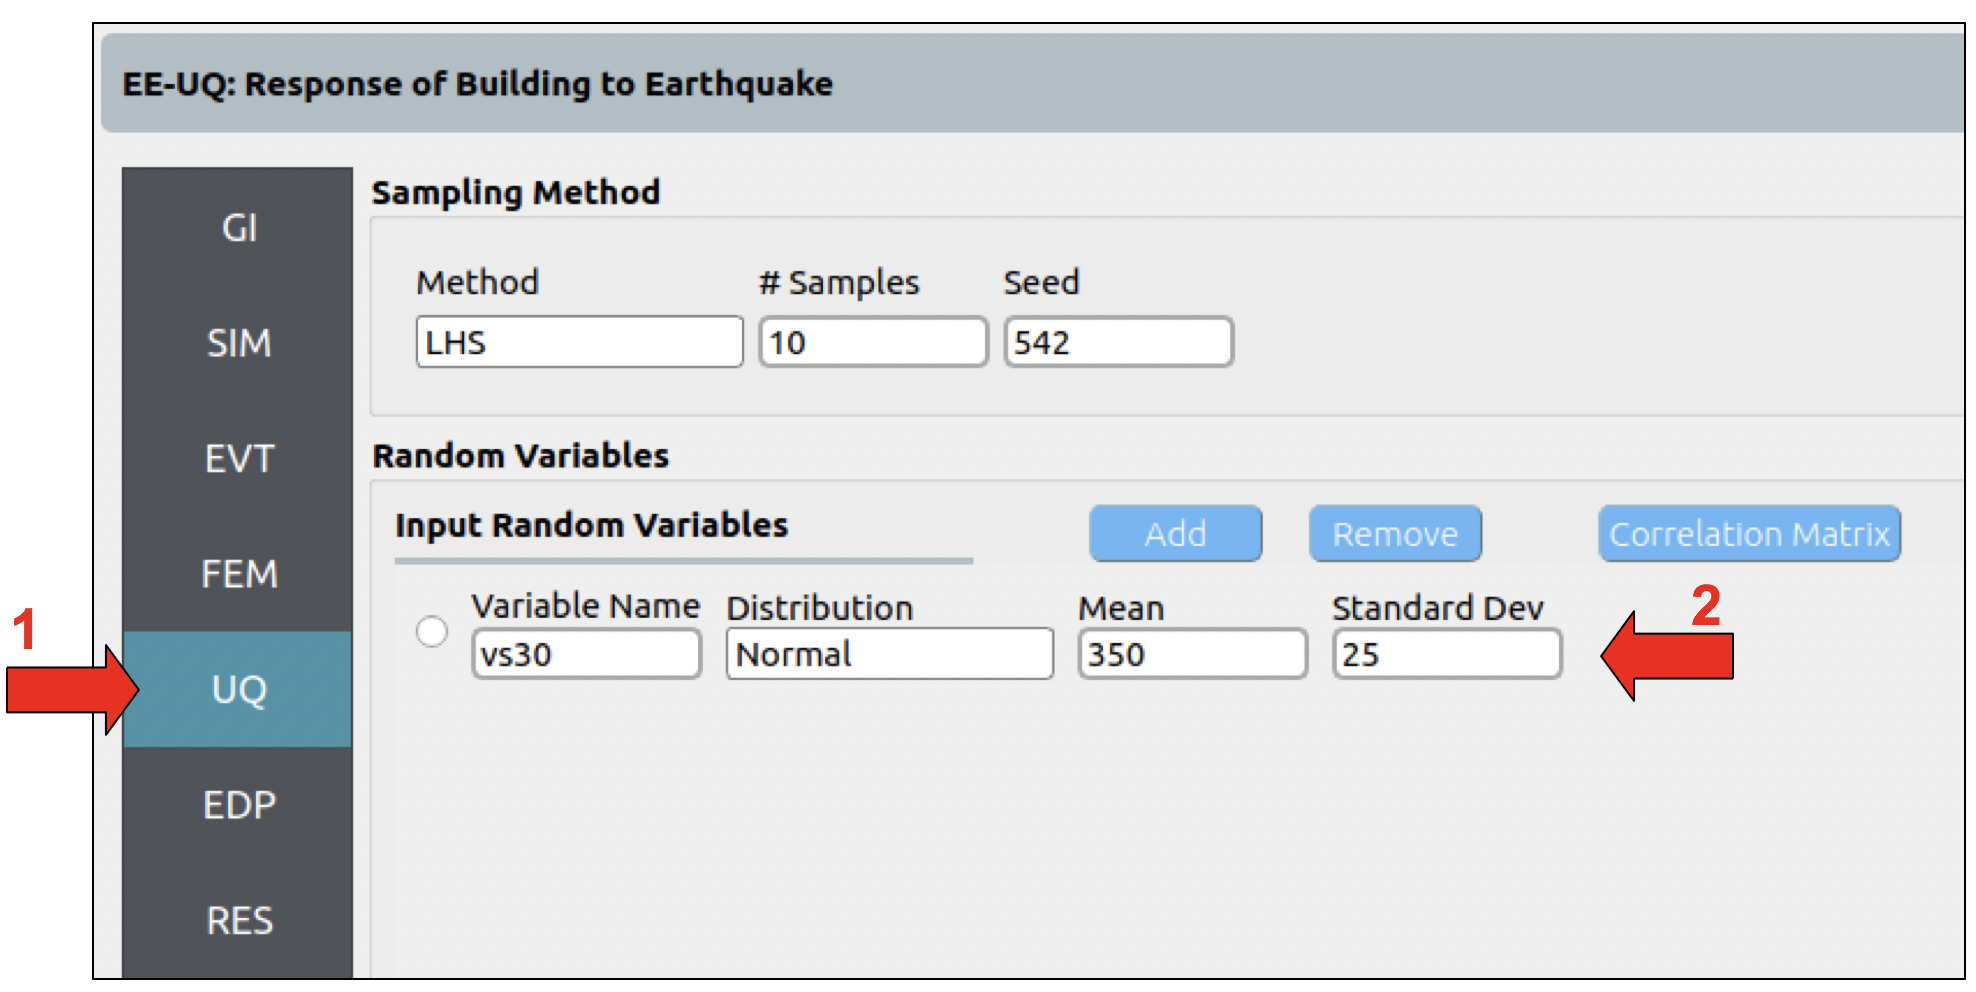
\includegraphics[width=0.7\textwidth]
    {installation/figures/test_input_uq.png} }
  \caption{Specifying distribution type and parameters for random
  variables in analysis\textemdash only $V_{s30}$ in this case}
  \label{fig:input_uq}
\end{figure}
}{}
\softwareSwitch{WE-UQ}{
\begin{figure}[!htbp]
  \centering {
    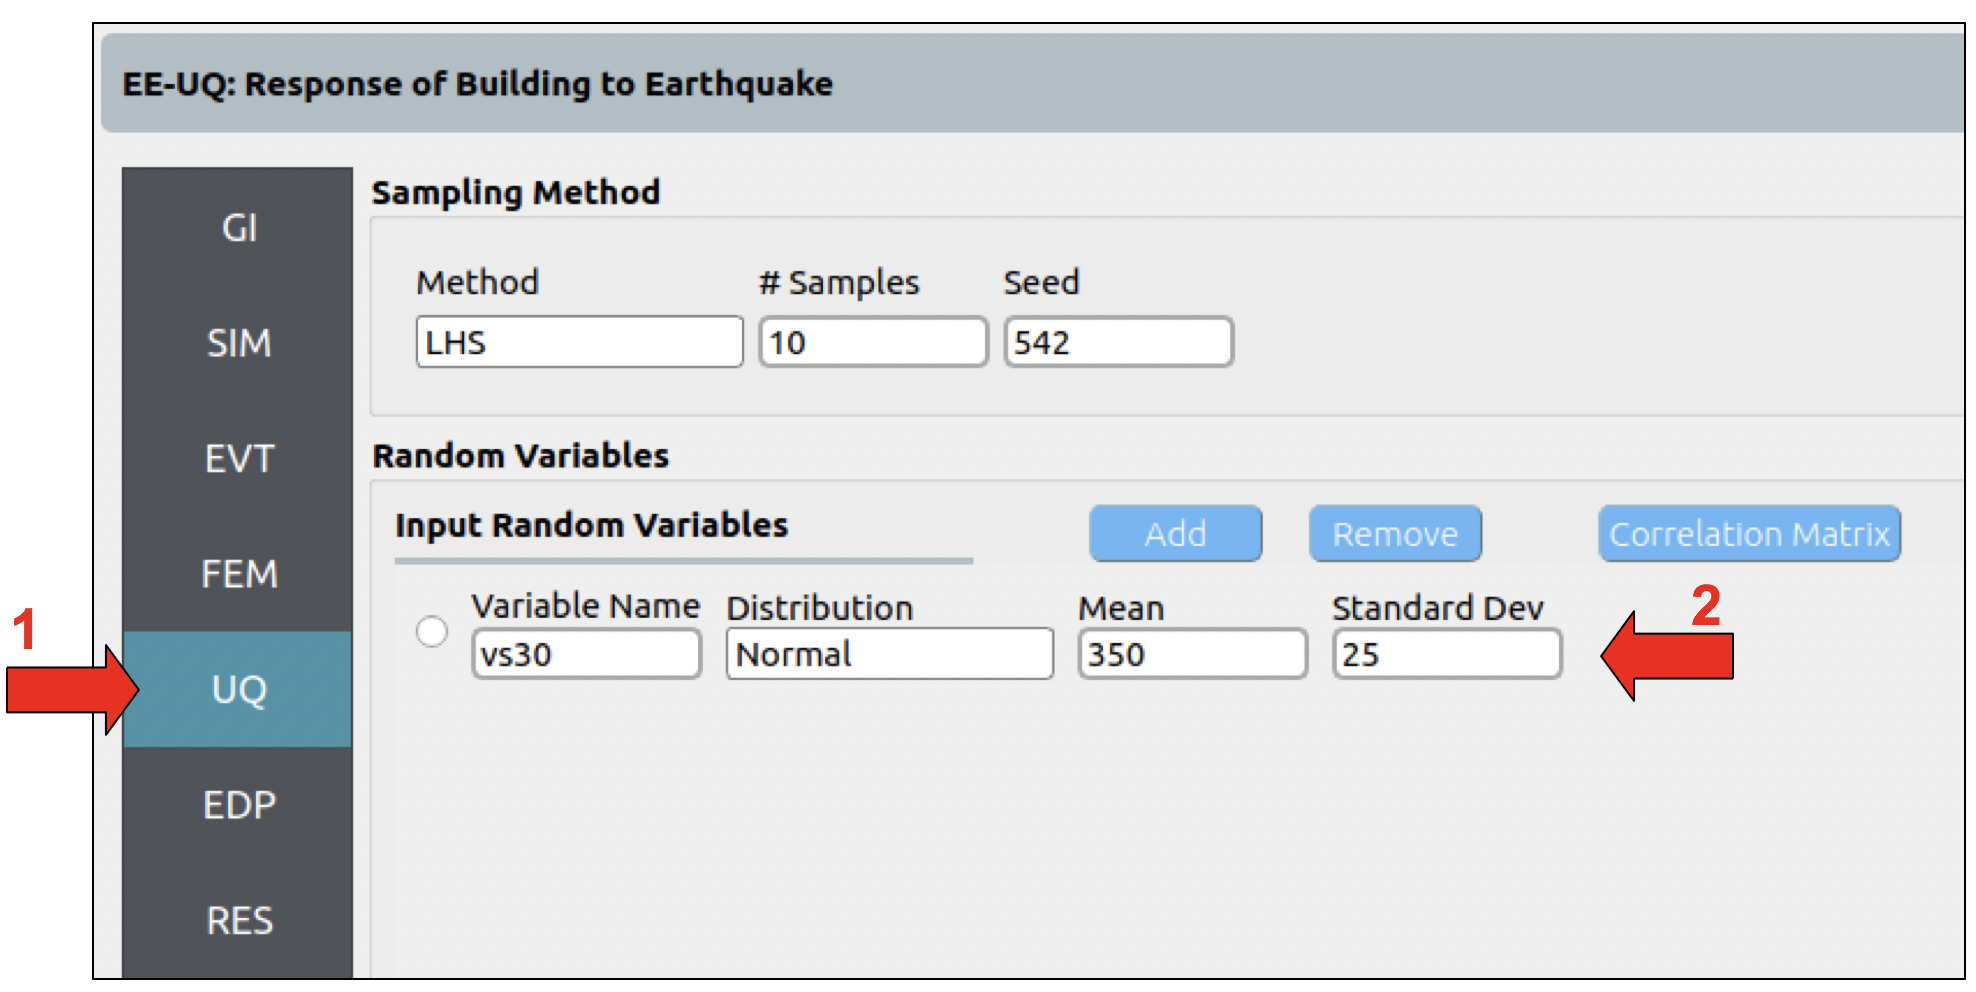
\includegraphics[width=0.7\textwidth]
    {installation/figures/test_input_uq.png} }
  \caption{Specifying distribution type and parameters for random
  variables in analysis\textemdash only $V_{s30}$ in this case}
  \label{fig:input_uq}
\end{figure}
}{}

\softwareSwitch{PBE}{
The last step before running the analysis is to set up the models for damage and loss assessment. Navigate to the \texttt{DL} tab and select \texttt{HAZUS MH} as the loss assessment method to use. Set up the models according to \Cref{fig:input_dl}.
\begin{figure}[!htbp]
  \centering {
    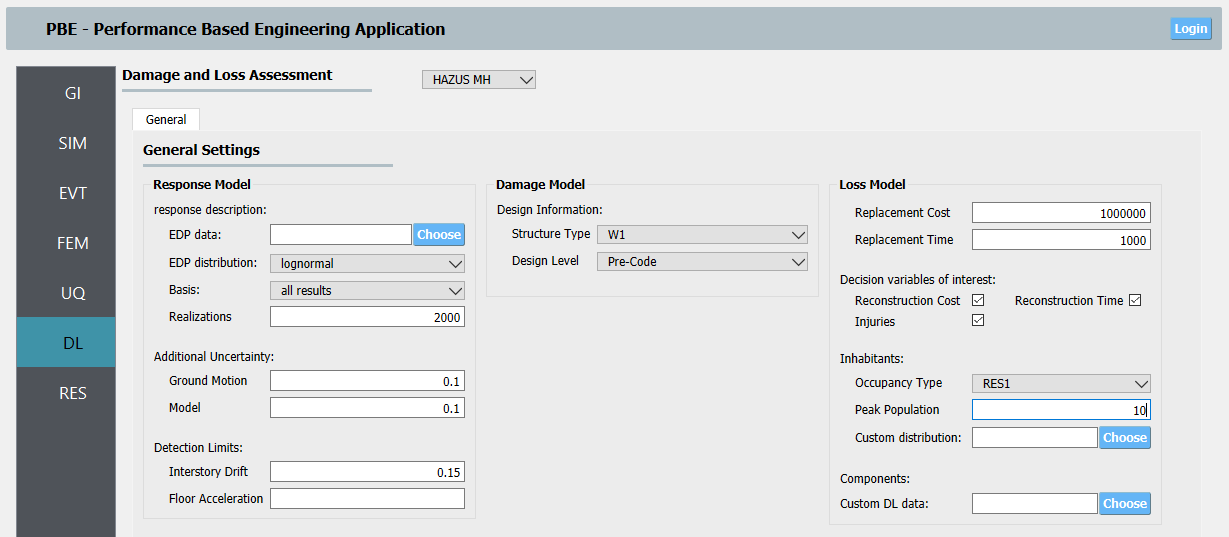
\includegraphics[width=0.95\textwidth]
    {installation/figures/test_input_dl.png} }
  \caption{Specifying the damage and loss model for the analysis.}
  \label{fig:input_dl}
\end{figure}
}{}

Now, click on the \texttt{RUN} button, which will automatically start the calculations.

\softwareSwitch{PBE}{
\begin{figure}[!htbp]
  \centering {
    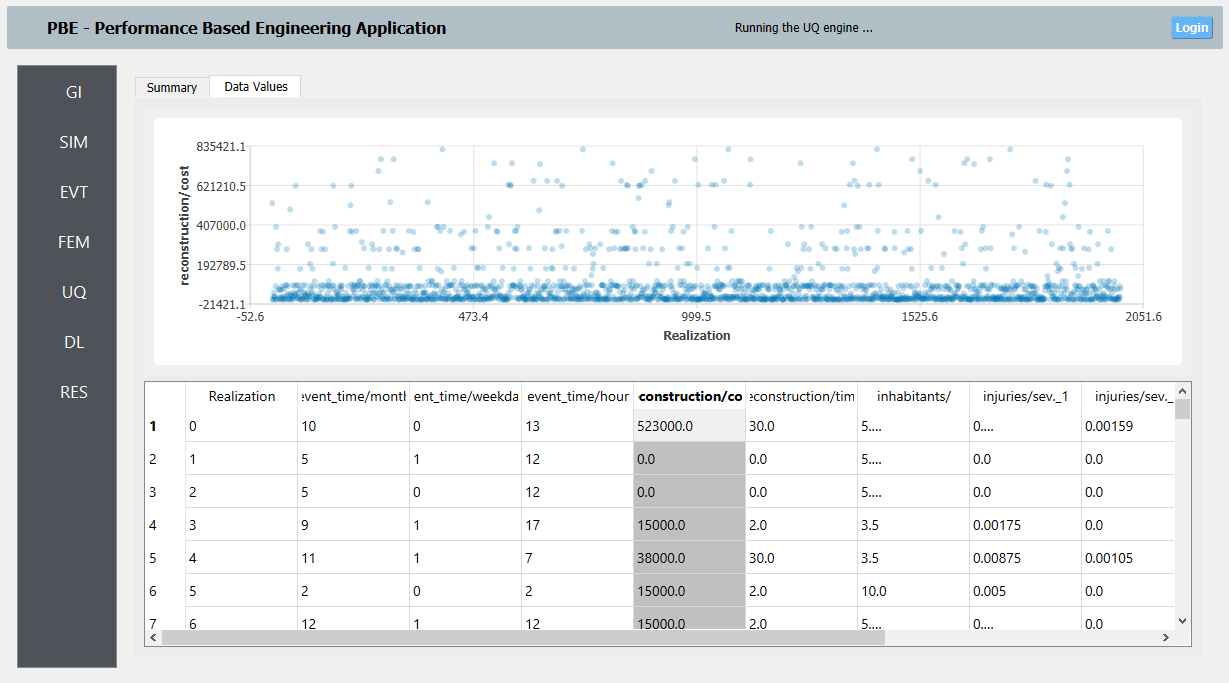
\includegraphics[width=0.95\textwidth]
    {installation/figures/test_uq_res_pbe.png} }
  \caption{Results for test analysis. This tab will open automatically
  when the analysis completes, indicating a successful installation}
  \label{fig:show_results}
\end{figure}
}{}

\softwareSwitch{EE-UQ}{
\begin{figure}[!htbp]
  \centering {
    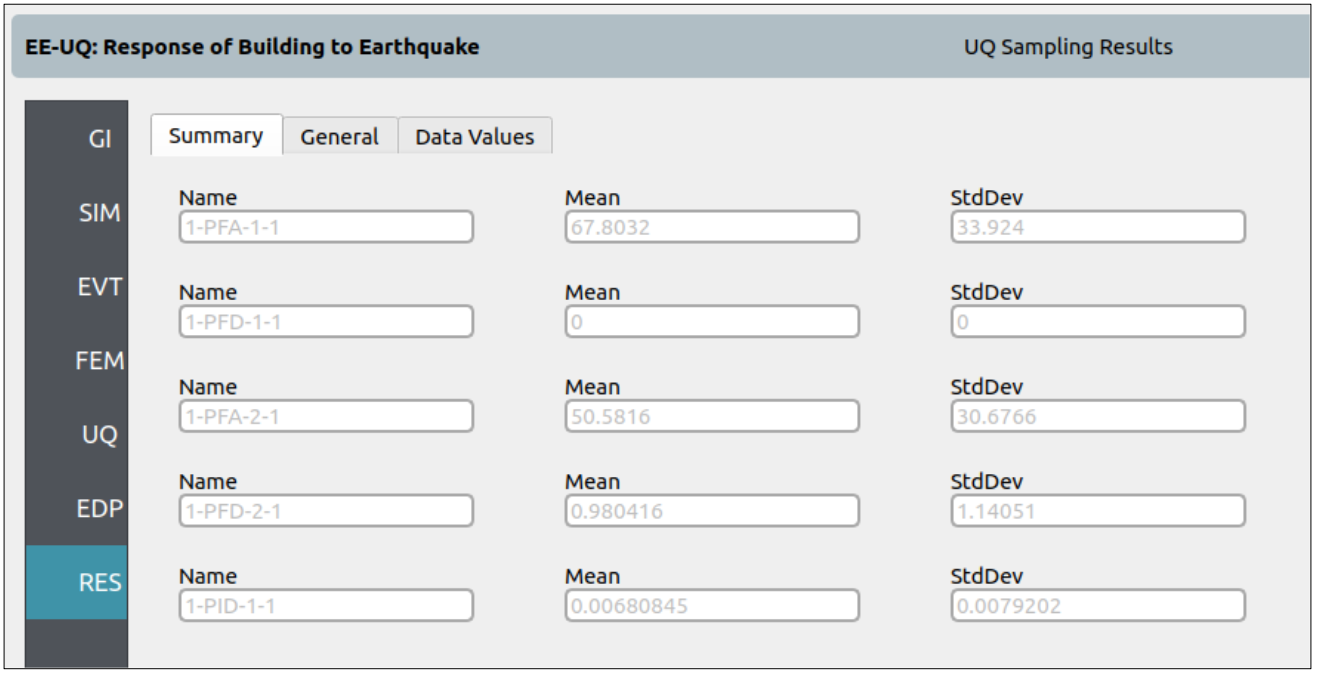
\includegraphics[width=0.7\textwidth]
    {installation/figures/test_uq_res.png} }
  \caption{Results for test analysis. This tab will open automatically
  when the analysis completes, indicating a successful installation}
  \label{fig:show_results}
\end{figure}
}{}

\softwareSwitch{WE-UQ}{
\begin{figure}[!htbp]
  \centering {
    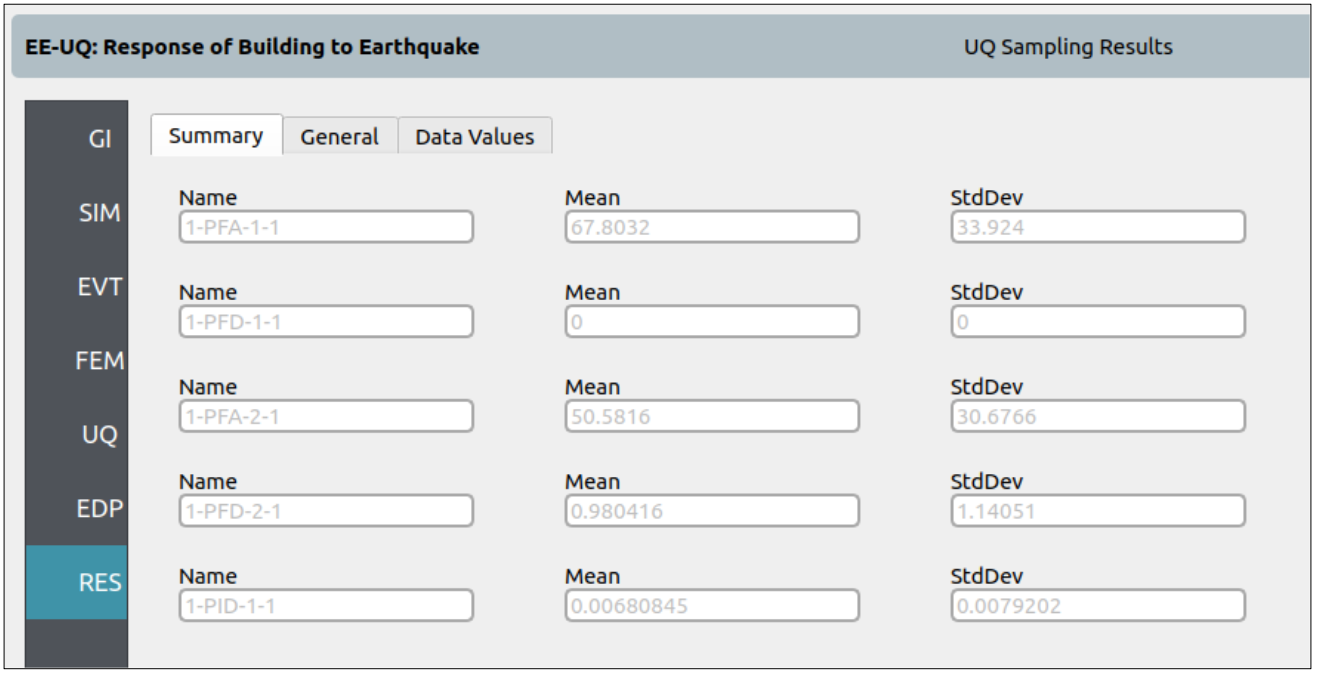
\includegraphics[width=0.7\textwidth]
    {installation/figures/test_uq_res.png} }
  \caption{Results for test analysis. This tab will open automatically
  when the analysis completes, indicating a successful installation}
  \label{fig:show_results}
\end{figure}
}{}

If successful, the application will pause briefly while it runs the
analysis before automatically displaying the simulations results in
the \texttt{RES} tab, as shown
in \Cref{fig:show_results}. Remember, the results shown
in \Cref{fig:show_results} most likely will not be the same as
those from your local test since $V_{S_{30}}$ is a random variable and
the values realized in the simulations will be different while still
following the same distribution. In any case, if the simulations
completed and the \texttt{RES} tab is showing simulation results, then
the \texttt{\getsoftwarename{}} App is properly installed and configured.

}
%===============================================================================



\chapter{Usage}
\label{chap:usage}
%\section{User Interface}
The user interface (UI), as shown in \Cref{fig:generic_ui}, is where the analysis
is configured and managed. Here, the user is able to provide the necessary
parameters to set up the simulation, start the simulation both locally and
remotely, and view the simulation results. The interface contains several
separate areas:

\softwareSwitch{PBE}{
\begin{figure}[!htbp]
  \centering {
    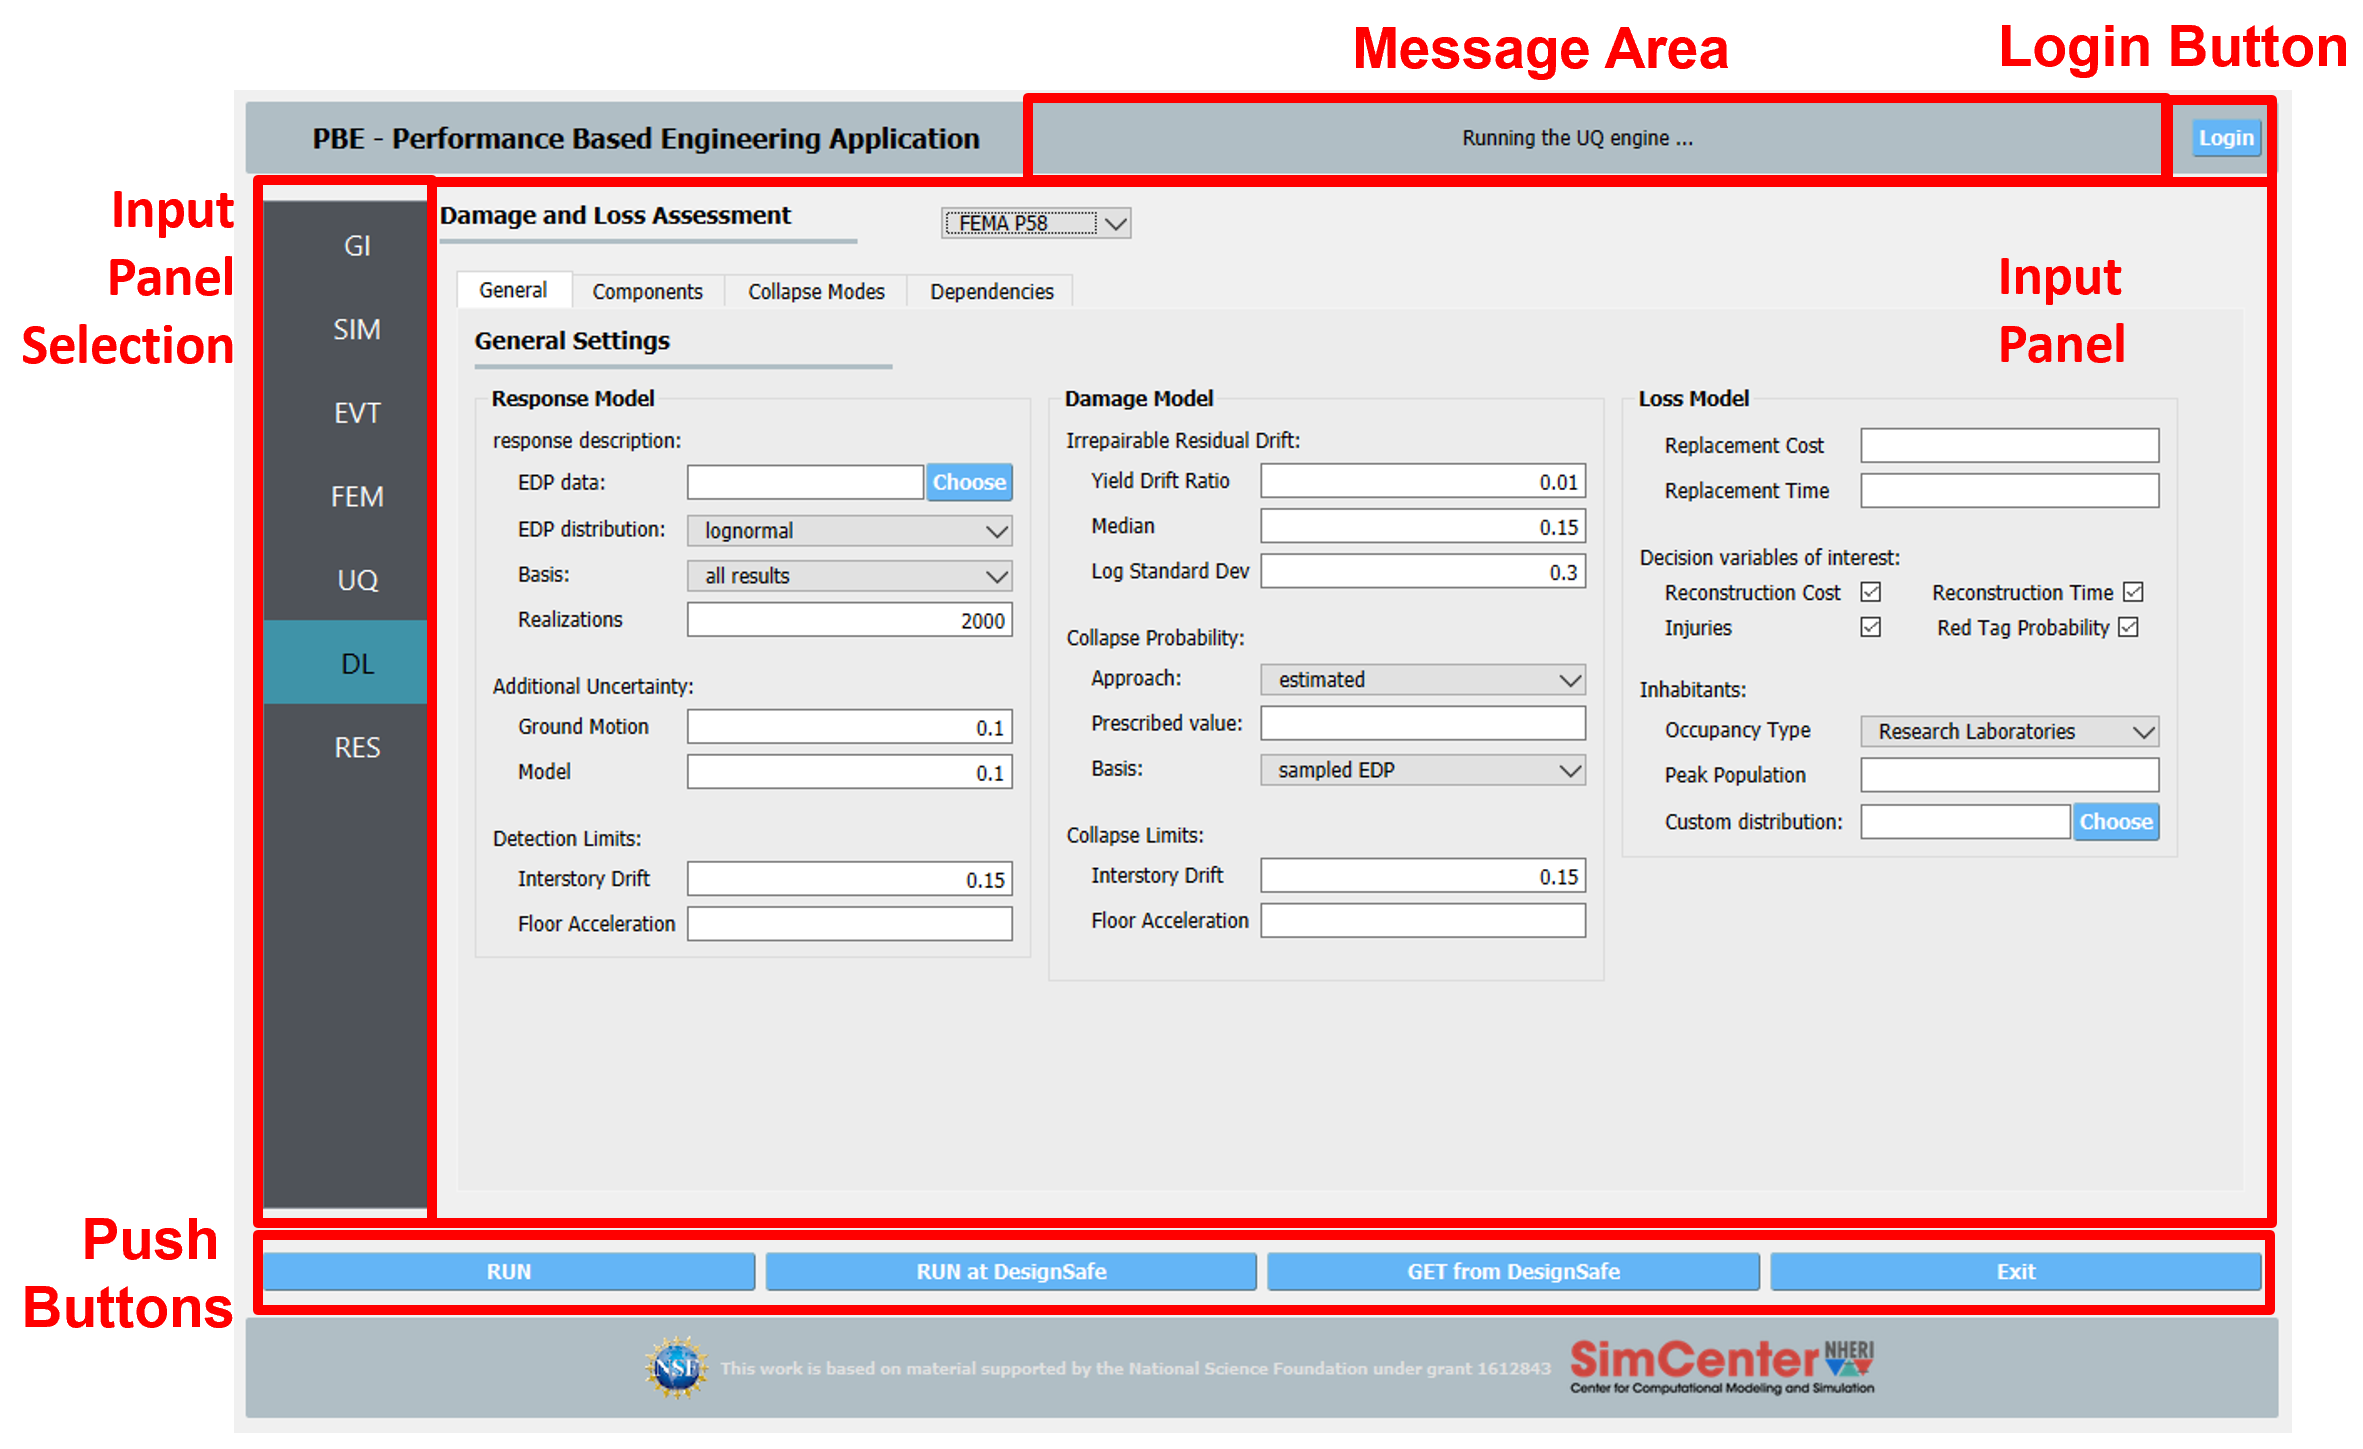
\includegraphics[width=0.95\textwidth]
    {usage/figures/pbePanel.png} }
  \caption{The User Interface (UI)}
  \label{fig:generic_ui}
\end{figure}
}{
\begin{figure}[!htbp]
  \centering {
    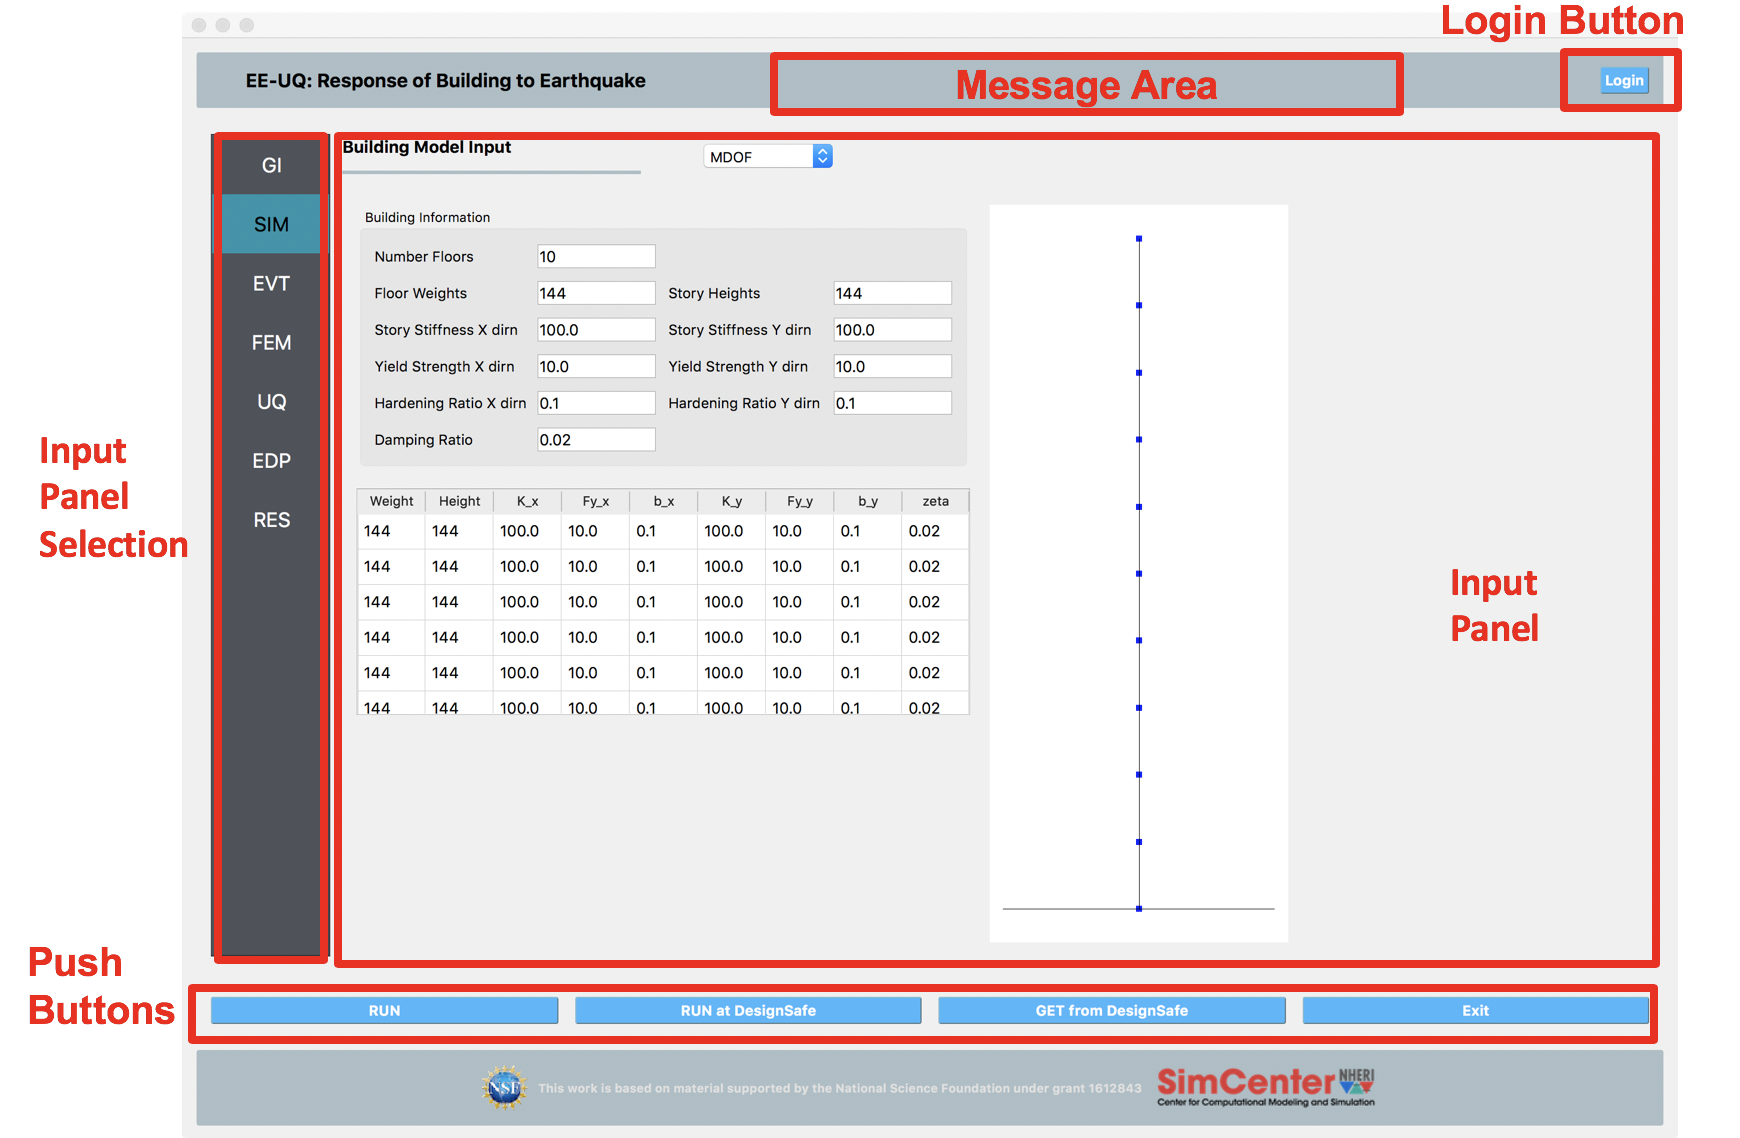
\includegraphics[width=0.95\textwidth]
    {usage/figures/eePanel.png} }
  \caption{The User Interface (UI)}
  \label{fig:generic_ui}
\end{figure}
}

\begin{enumerate}
\item Input Panel Selection: This area on the left side provides the
  user with a selection of items to choose from:
\begin{enumerate}
  \item GI: General Information (\Cref{sec:generalInfo}), for specification of building
    description, location and units.
  \item SIM: Structure Information Model (\Cref{sec:structuralInfo}), for description of the
    building model.
    \softwareSwitch{WE-UQ}{
      \item EVT: Event (\Cref{sec:event}), for selecting the input wind loading for the building.    
    }{
      \item EVT: Event (\Cref{sec:event}), for selecting the input earthquake motions for the building.    
    }
  \item FEM: Finite Element Method (\Cref{sec:fem}), for specifying the options for structural response simulation.
  \item UQ: Uncertainty Quantification (\Cref{sec:uq}), for defining the distribution
    of the random paramaters and UQ method analysis options.

\softwareSwitch{PBE}{
 \item DL:  Damage and Loss Model (\Cref{sec:dl}), for specification of the damage and loss model parameters.
}{ 
  \item EDP: Engineering Demand Parameters (\Cref{sec:edp}), for 
  specification of output response quantities.
}

  \item RES: Results output (\Cref{sec:results}), for looking at the results.
\end{enumerate}

Selecting any of these will change the input panel presented.

\item Input Panel: This is the large central area of the UI where the
  user provides input for the application chosen and where thay can view the
  results. For example, if the user had selected UQ in the input panel
  selection, it is in this panel that the user would provide details
  on the distributions associated with each random variable or select
  the sampling method to use and provide the options necessary to run
  that method.

\item Push Buttons: This is the area near the bottom of the UI in
  which 4 buttons are presented to the user:

\begin{enumerate}
\item RUN – Run the simulation locally on the user’s desktop machine.
\item RUN at DesignSafe – Process the information, and send to
  DesignSafe. The simulation will be run there on a supercomputer, and results
  will be stored in the user's DesignSafe jobs folder.
\item GET from DesignSafe – Obtain the list of
  jobs for the user from DesignSafe and select a job to download from that list.
\item Exit: Exit the application.
\end{enumerate}

The first 3 of the above buttons and their use are discussed in more detail in \Cref{sec:push_buttons}.

\item Login Button: The Login Button is at the top right of the UI. Before the user can launch any jobs on DesignSafe, they must
  first login to DesignSafe using their DesignSafe login and
  password. Pressing the login button will open up the login window
  for users to enter this information. Users can register for an
  account on
  the \href{https://www.designsafe-ci.org/account/register/}{DesignSafe
  webpage}.

\item Message Area: While the application is running, error and status messages will be displayed here, in the top center of the user interface.

\end{enumerate}


\section{GI: General Information}
\label{sec:generalInfo}
The user here provides information about the building and the units
the user will work with. The widget contains 4 separate frames,
as shown in \Cref{fig:gi_overview}:

\begin{enumerate}
\item Building Information: Collects general information about the building: name, type, and year of construction.
\item Properties: Collects information about number of stories, width, depth, plan area and height of the building.
\item Location: Collects information about the location of the building. This information is used in some event widgets to obtain events specific to the building location.
\item Units: Collects information about the units for the inputs and outputs. Some widgets will require inputs in different units. Those widgets will display units beside those special entry fields.
\end{enumerate}

\begin{figure}[!htbp]
  \centering {
    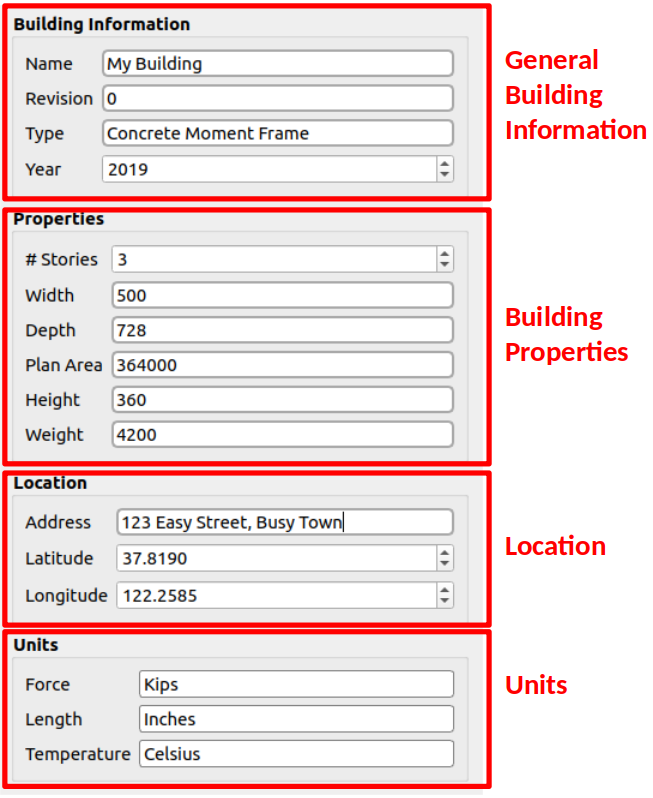
\includegraphics[width=0.5\textwidth]
    {usage/figures/gi.png} }
  \caption{General Information Input Panel}
  \label{fig:gi_overview}
\end{figure}



\section{SIM: Structural Information Model}
\label{sec:structuralInfo}
The user here defines the structural system of the
building. The  structural system is the part of the building provided
to resist the gravity loads and those loads arising from the natural hazard. 
There are a number of backend applications provided for this part of the workflow, 
each responsible for defining the structural analysis model. The user can select 
the application to use from the drop-down menu at the top of this panel. As the 
user switches between applications,
the input panel changes to reflect the inputs each particular application requires. At present, there are two backend applications
available through the drop down menu: 

\begin{enumerate}
\item Multiple Degrees of Freedom (MDOF) (\Cref{sec:MDOF})
\item \texttt{OpenSees} (\Cref{sec:OpenSeesSIM})
\end{enumerate}

\subsection{Multiple Degrees of Freedom (MDOF)}\label{sec:MDOF}

This panel is provided for users to quickly create simple shear models
of a building. The panel, as shown in \Cref{fig:mdof} is divided
into 3 frames:
\begin{enumerate}
\item The top left frame allows the user to specify the number of stories and properties that are constant for every floor and story in the building. The following properties are available: floor weight, story height, torsional stiffness, initial stiffness, yield strength, and hardening ratio for each direction in each story. The user has the option of specifying values for eccentricty of mass in x and y directions, and eccentricities for the location of the response quantities. Here, the one and two directions are orthogonal $x$ and $y$ axes in plan view.
\item The lower left frame allows the user to override the structural parameters above for individual floors and stories.
\item The frame on the right is a graphical widget showing the current building. When entering data into the lower left frame, the stories corresponding to the data being modified are highlighted in red.
\end{enumerate}

\begin{figure}[!htbp]
  \centering {
    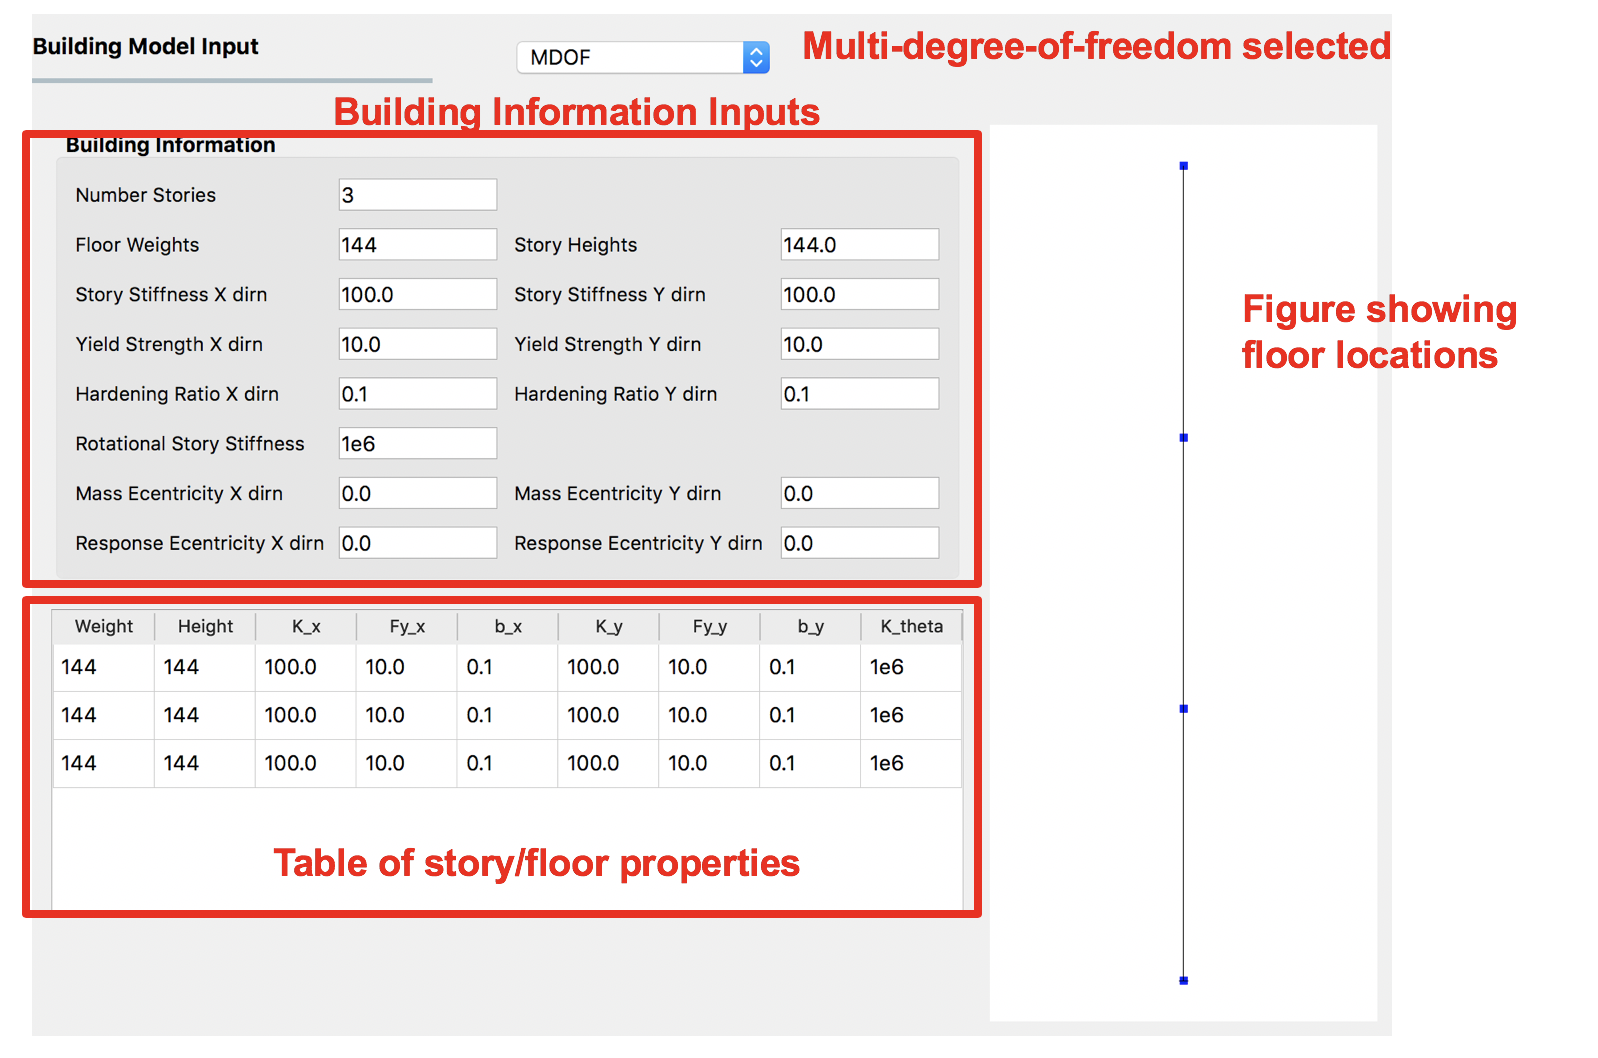
\includegraphics[width=0.8\textwidth]
    {usage/figures/mdof.png} }
  \caption{MDOF or Shear Building Model}
  \label{fig:mdof}
\end{figure}

Random Variables: Random Variables can be created by the user if they enter
a valid string instead of a number in the entry fields for any entry
except for the \emph{Number of floors}. The variable name entered will appear as
a Random Variable in the UQ panel; it is ther the user must specify the distribution 
associated with the Random Variable.

\subsection{\texttt{OpenSees}}\label{sec:OpenSeesSIM}
This panel is for users who have an existing \texttt{OpenSees} model of a
building that performs a gravity analysis and now they wish to subject that
building model to one of the \texttt{EVT} options provided. The input panel
for this option is shown in \Cref{fig:figure3}. Users need to provide three pieces of information:
\begin{enumerate} 
\item Main OpenSees Script: The main script that contains the building
  model. This script should build a model and perform any gravity
  analysis of the building that is required before the event is
  applied.
\item Response Nodes: A list of node numbers that define a column line of interest for which
  the responses will be determined. The column nodes should be in
  order from ground floor to roof. 
  The EDP workflow application\softwareSwitch{PBE}{}{, described
  in \Cref{sec:edp},} uses this information to determine nodes at which
  displacement, acceleration, and story drifts are calculated.
\item An entry for the dimension of the model (i.e., 2D or 3D). This
  information is used when \softwareSwitch{WE-UQ}{wind loads}{ground motions} are applied.
\item entry for the number of degrees of freedom at each node in the model.
\end{enumerate}

\begin{figure}[!htbp]
  \centering {
    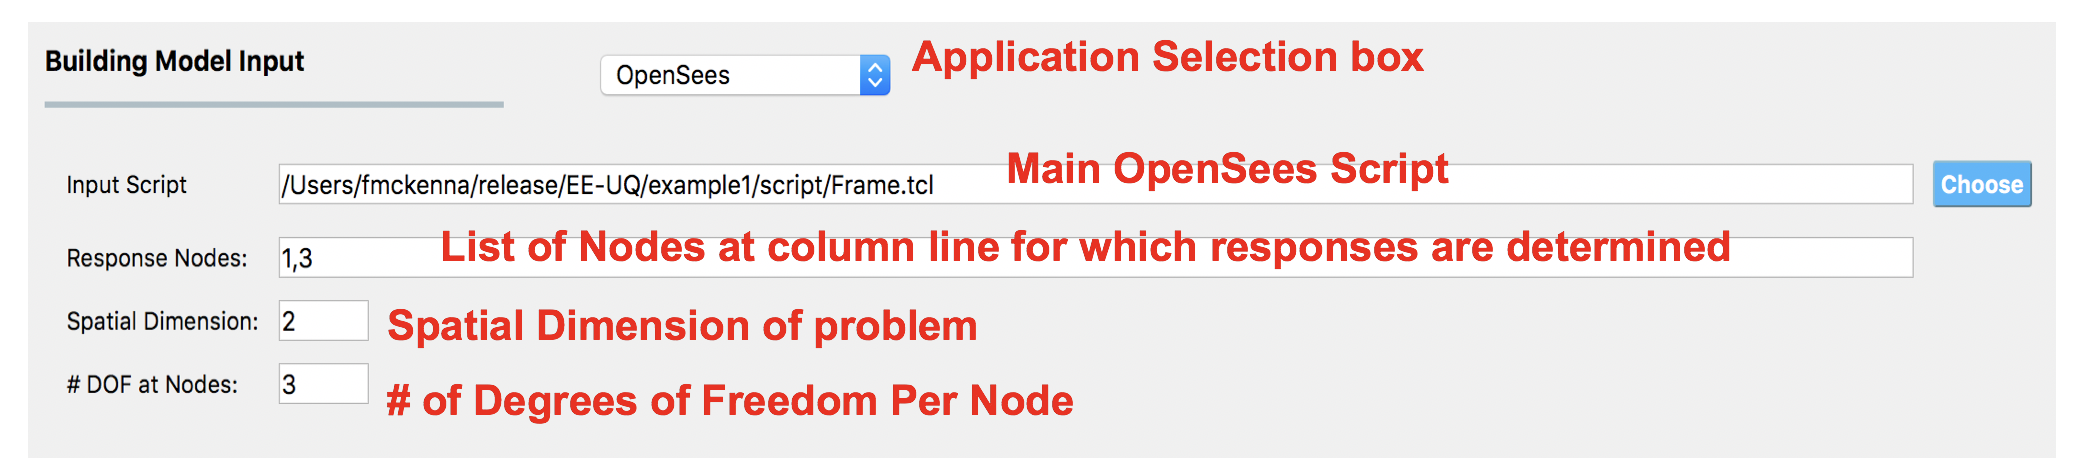
\includegraphics[width=0.8\textwidth]
    {usage/figures/openSees.png} }
  \caption{\texttt{OpenSees} Model}
  \label{fig:figure3}
\end{figure}


Random Variables: In \texttt{OpenSees} there is an option to set
variables to have certain values using the \texttt{pset} command, e.g
\texttt{pset a 5.0} will set the variable a to have a value 5 in the
\texttt{OpenSees} script. In \texttt{\getsoftwarename{}}, any variable
found in the main script to be set using the \texttt{pset} command
will be assumed to be a Random Variable. As such, when a new main
script is loaded all variables set with \texttt{pset} will appear as
Random Variables in the UQ panel.


\section{EVT: Event}
\softwareSwitch{WE-UQ}{
\label{sec:event}
The event panel presents the user with a drop-down menu with a list of
available event applications. Event applications are applications
that, given the building and user supplied data inputs, will generate
a list of events (i.e., typically time-dependent loads that represent natural disasters) for the building. The following options
are available in the drop-down menu:

\begin{enumerate}
\item Stochastic Wind Event (\Cref{subsec:stochastic_wind})
\item CFD Basic (\Cref{subsec:cfd_basic})
\item CFD Expert (\Cref{subsec:cfd_expert})
\item DEDM HRP (\Cref{subsec:dedm_hrp})
\item Low Rise TPU (\Cref{subsec:lowRiseTPU})
\item Wind Tunnel Data (\Cref{subsec:windTunnelExperiment})
\item Multiple Existing(\Cref{subsec:multiple_existing})
\end{enumerate}

\subsection{Stochastic Wind}
\label{subsec:stochastic_wind}
This option allows users to generate synthetic wind velocity time
histories for target wind loading. In order to do so, the stochastic
wind model is selected from the drop-down menu, as shown in
\Cref{fig:stochastic_wind_loading}. Depending on the model selected, the
user will be asked to enter the parameters describing the wind loading
scenario that the synthetic time history should emulate. In the
current release, users can only select the model derived by Wittig \&
Sinha (1975) \cite{wittig1975simulation}. Additionally, users can
provide a seed for the stochastic wind generation if they desire the
same suite of synthetic time histories to be generated on multiple occasions.
If the seed is not specified, a different realization of the time
history will be generated for each run based on the input
parameters. The backend application that generates the stochastic
wind loads relies on \texttt{smelt}, a modular and extensible C++
library for generating stochastic time histories. Users interested in
learning more about the implementation and design of \texttt{smelt}
are referred to its
\href{https://github.com/NHERI-SimCenter/smelt}{GitHub repository}.

All input parameters can be specified as random variables by entering
a string in the parameter field. Please note that information for the
inputs that are identified as random variables needs to be provided in
the \texttt{UQ} tab.

\begin{figure}[!htbp]
  \centering {
    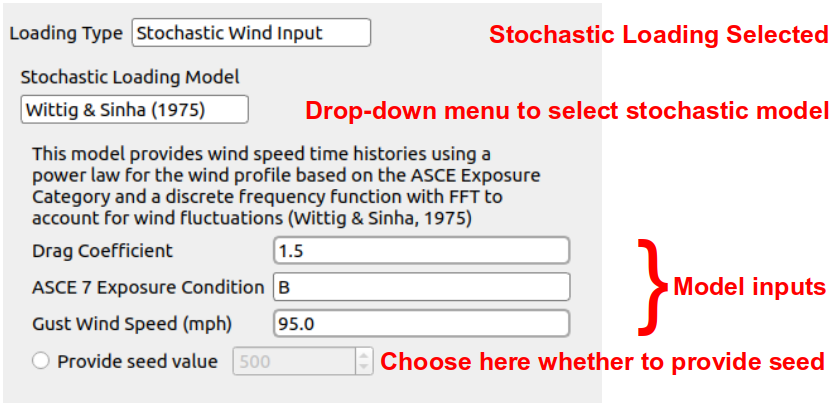
\includegraphics[width=0.8\textwidth]
    {usage/figures/stochastic_wind_loading.png} }
  \caption{Stochastic Wind Loading Event}
  \label{fig:stochastic_wind_loading}
\end{figure}


\subsection{CFD Basic}
\label{subsec:cfd_basic}
This event facilitates generating a CFD model for wind flow around a building. A template is provided to the user to generate an OpenFOAM model based on a set of parameters for mesh generation and CFD simulation. The user needs to specify the domain size, mesh size, boundary conditions, simulation parameters and the method for extracting wind forces on the building as shown in \Cref{fig:cfd_template}.

\begin{figure}[!htbp]
    \centering {
        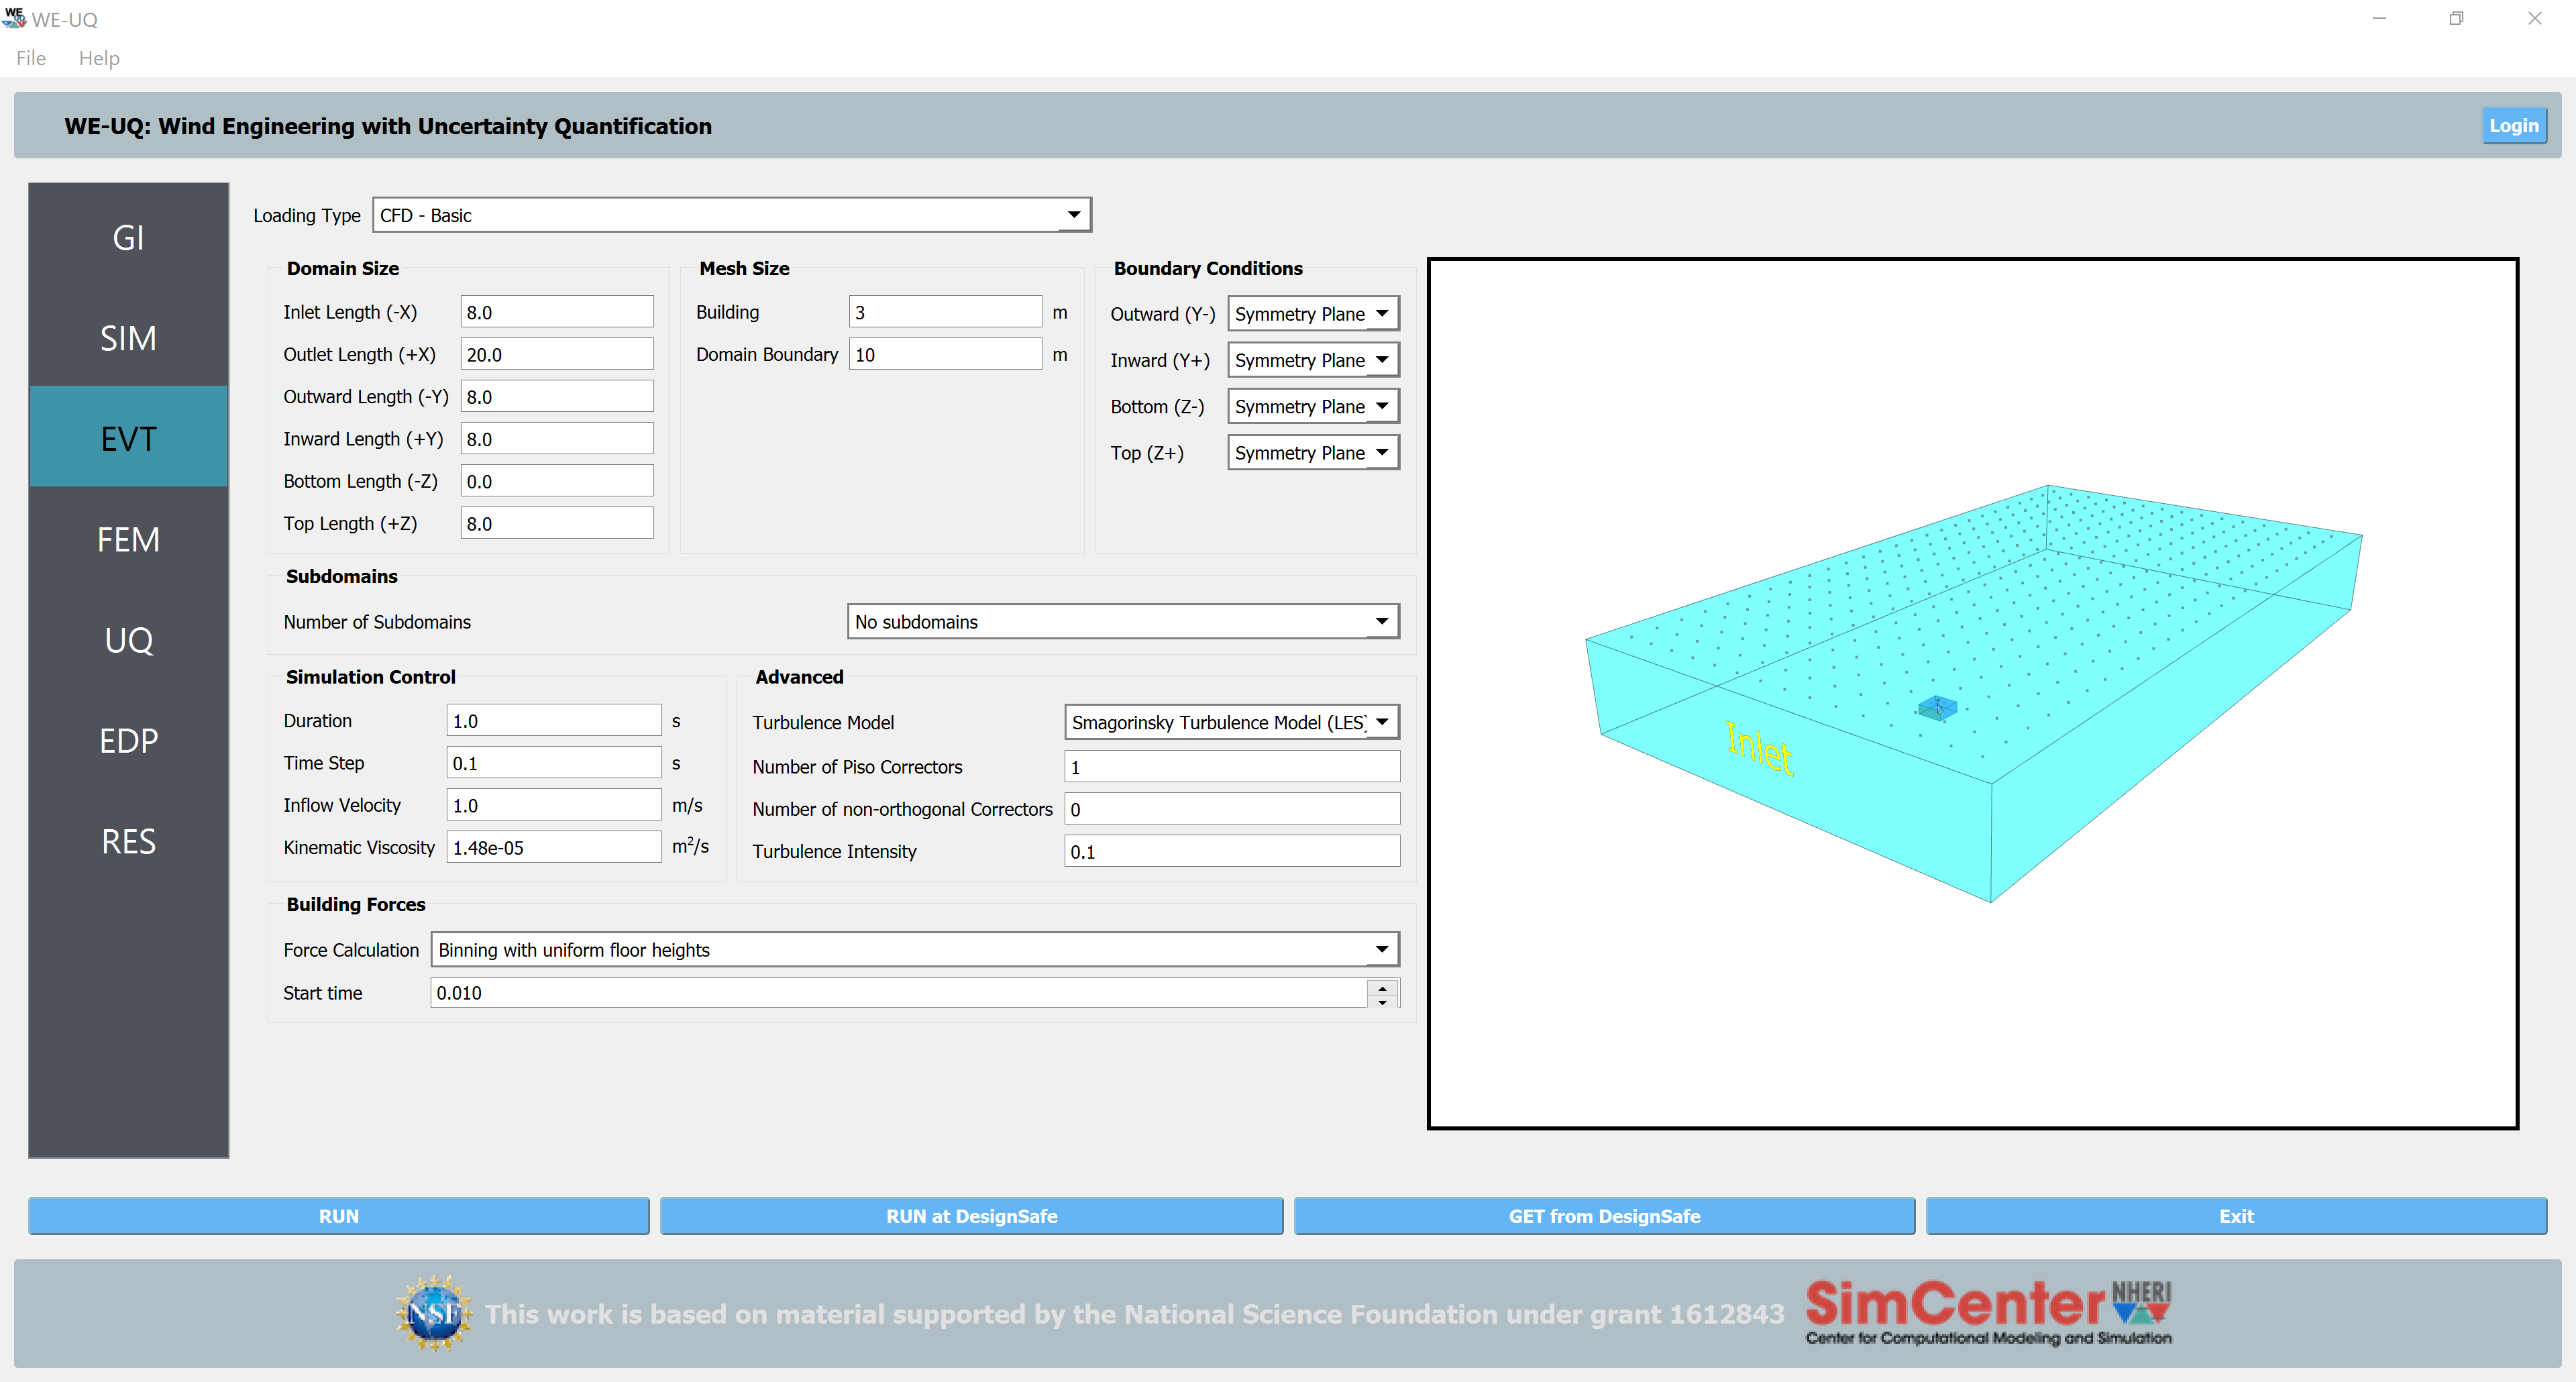
\includegraphics[width=0.95\textwidth]
        {usage/figures/cfd_template.png} }
    \caption{CFD Template Event}
    \label{fig:cfd_template}
\end{figure}

The following are the steps the user should follow to use the CFD template:

\begin{enumerate}
\item Specify the domain size in different directions using the input fields in the domain size group. It is important to note here that the size is relative to the building size. A three dimensional view is provided to allow the user to visualize the domain size. The 3D view should also indicate the location of the wind flow inlet.

\item Prescribe mesh sizes at the building surface and the outer edge of the wind field boundary. Mesh sizes are specified in meters. Users can visualize the prescribed mesh size compared to the domain and building sizes, only for the top surfaces.

\item The next step is to specify the boundary conditions on the sides, top and bottom of the domain. The user can select between wall or symmetry plane boundary conditions.

\item Optionally, the user can also specify up to three inner sub-domains. The desired mesh size and dimensions of sub-domains can be specified and they follow the same convention as the main domain.

\item Basic and advanced simulation parameters needs to be specified. The user can specify the total time, time step, wind velocity, turbulence model used in the OpenFOAM CFD simulation.

\item  Finally, the user needs to specify how the force on the building are extracted. Currently, the only method supported is to group forces on the building into bins of equal height, where each bin corresponds to a building floor. In addition, a start time for the applying the forces on the building model has to be specified, forces before that time will not be used. This allows the user to ignore force values in the beginning of the CFD simulation as they may not be accurate.

\end{enumerate}

It has to be noted that this event can only run remotely at DesignSafe-CI, and is not supported to be run on the local computer. Once the analysis is run a mesh is generated using Gmsh based on the meshing parameters specified by the user, then and OpenFOAM model is generated, analyzed and its output will be used to extract forces acting on the building, assuming the building is a rigid body. It is also important to note that intermediate meshing and CFD simulation results are available in the output archive folder for the user to inspect, if needed. 


\subsection{CFD Expert}
\label{subsec:cfd_expert}
This option allows users to obtain wind forces utilizing an existing OpenFoam model 
that was uploaded to Design-Safe data depot. 
This is done by coupling the OpenFOAM model and the building model in a weak form, 
where the CFD analysis is executed first, then building forces are extracted and applied to the building model.
This initial version is limited in scope due to the following assumptions:

\begin{itemize}
    \item The OpenFOAM model has a patch with the name \textit{building} that represents the building envelope.
    \item Only horizontal forces are applied to the building model, the vertical force and moments are not considered.
    \item The building forces are extracted using the binning feature in OpenFOAM force module and thus, it is
          assumed that all the floors are of equal heights.
    \item OpenFOAM solvers supported are limited to \textit{pisoFOAM}.
    \item Meshing is performed using the \textit{blockMesh} tool.
    \item No uncertainty is considered in the CFD analysis.
\end{itemize}

It is important to note that this type of event is only supported when running the simulation at DesignSafe and 
does not run on the local computer.
The backend applications used in WE-UQ create a copy of the OpenFOAM case directory provided by the user,
then modify the post-processing stage in the case to output the forces acting on the building, for each floor level.
\Cref{fig:cfd_expert} shows input parameters required for using the CFD expert event. It is important to note
that this event requires the user to have an OpenFOAM case uploaded to DesignSafe data depot. For that reason, 
the widget is disabled when the user is not logged into DesignSafe. Once the user signs in, the widget is enabled
and the input parameters can be changed. 

\begin{figure}[!htbp]
    \centering {
        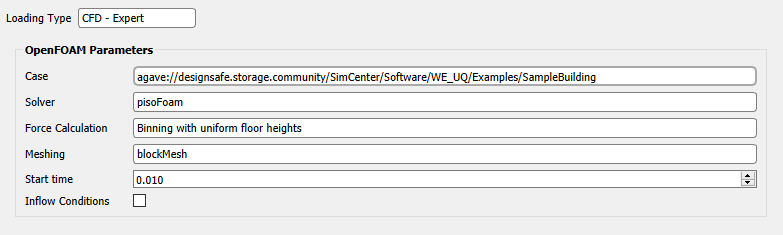
\includegraphics[width=0.8\textwidth]
        {usage/figures/cfd_expert.png} }
    \caption{CFD Expert Event}
    \label{fig:cfd_expert}
\end{figure}

There are at least 6 input parameters that needs to be provided by the user and can be summarized as follows:
\begin{itemize}
    \item \textbf{Case:} The remote path of the OpenFOAM case that was uploaded in advance to DesignSafe data depot.
    By default, this is set to an example case that is provided by the SimCebnter in the community directory.  
    \item \textbf{Solver:} The OpenFOAM solver that is used in the simulation.
    \item \textbf{Force Calculation:} The method used to calculate the forces acting on the building in the CFD analysis.
    \item \textbf{Meshing:} The meshing tool used for the provided OpenFOAM case. 
    \item \textbf{Start time:} The time in the CFD simulation to start extracting the forces on the buildings.
        Force values before that time are not used.
    \item \textbf{Inflow Conditions:} Whether or not the inflow conditions will be specified for the CFD simulation.   
\end{itemize}

If the user selects to specify the inflow conditions, the parameters for the inflow condition shown in \Cref{fig:cfd_expert_inflow}
will need to be specified.
This requires the application to download some of the case files and modify them before the simulation is started,
which is done automatically by the tool.

\begin{figure}[!htbp]
    \centering {
      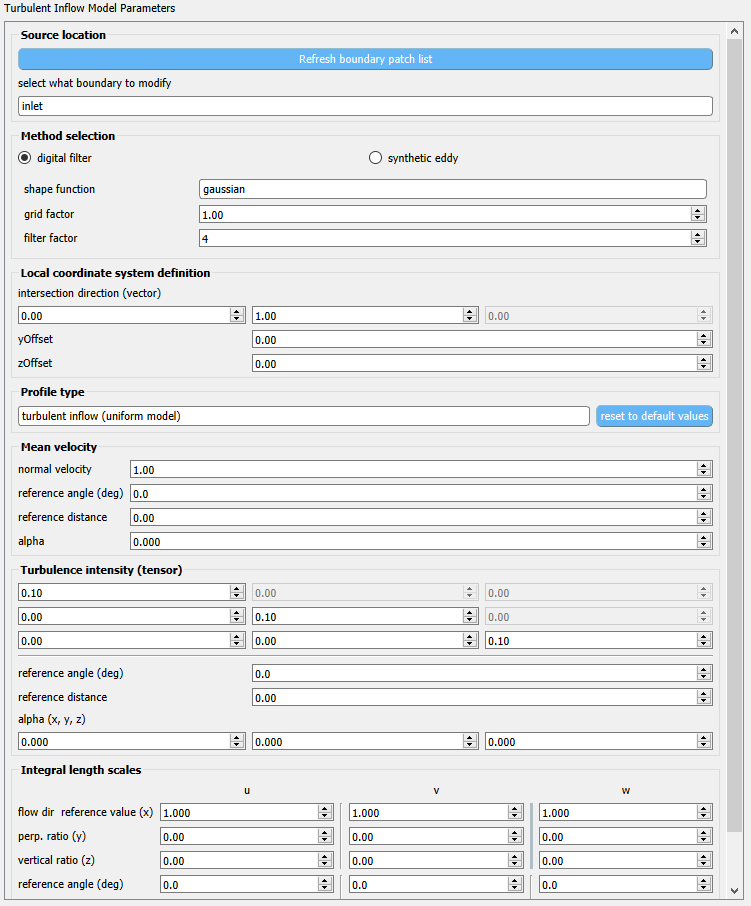
\includegraphics[width=0.8\textwidth]
      {usage/figures/cfd_expert_inflow.png} }
    \caption{Inflow Condition Parameters}
    \label{fig:cfd_expert_inflow}
\end{figure}

\subsection{DEDM HRP}
\label{subsec:dedm_hrp}
For this event type, full-scale floor loads are generated by a web service, 
\href{http://evovw.ce.nd.edu/DEDM_HRP/DEDMP_INT_v3_4evo.html}{DEDM HRP} a Database-Enabled Design module 
for High-Rise buildings using Pressure data. The loads  are downloaded and then applied to the 
building when either of the run buttons are pressed.

To understand the inputs, it is necessary to understand that the DEDM-HRP website itself 
utilizes the aerodynamic database compiled at the Tokyo Polytechnic 
University, Japan (referred to simply as TPU database). THE TPU database contains data 
for a variety of building  configurations of different building width (B), depth (D), and 
height (H) ratios (B:D:H ratios), tested for various incident wind direction and exposure conditions.
 The TPU database comprises a total of 394 test cases, derived for 3 square/rectangular cross-sectional 
shapes, 4 to 5 model heights, 1 to 2 exposure categories and 11 to 21 incident wind directions of 5 
degree increments. 

\begin{figure}[!htbp]
  \centering {
    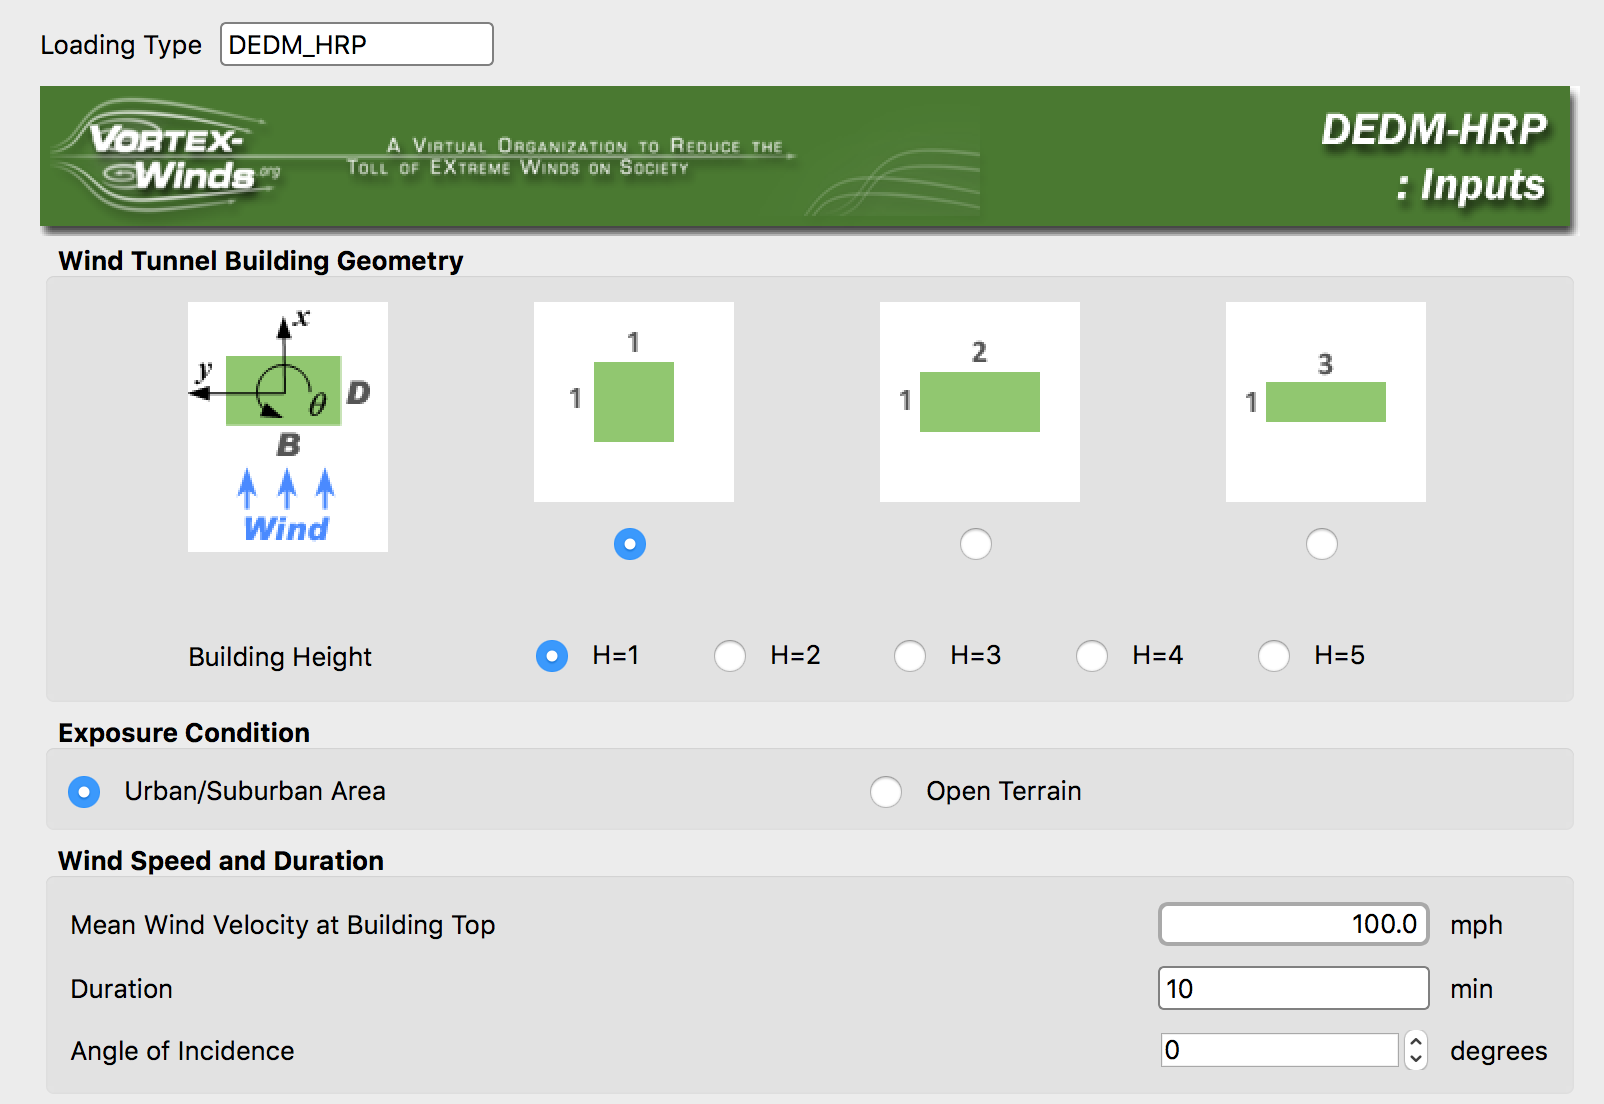
\includegraphics[width=0.8\textwidth]
    {usage/figures/dedmHRP.png} }
  \caption{DEDM HRP Wind Loading Event}
  \label{fig:dedm_hrp}
\end{figure}

In the inputs for the event, as shown in figure \Cref{fig:dedm_hrp} require the user to specify which 
of these tests to use:
\begin{enumerate} 
\item The user to select from one of the three cross sectional shapes.
\item The user specifies one of five building heights.
\item One of two exposure conditios: urban/suburban terrain (alpha = 0.25)
and open terrain (alpha = 0.167), which would correspond to Exposure B and C, respectively, 
as defined in ASCE 7 standard.
\item Mean Wind Speed at Top of Building: The basic wind speed in the ASCE standard 
(e.g., ASCE 7-16) is defined as 3-sec gust at 10 m height. However, the DEDM-HRP asks
the inputs of mean wind speeds at the top of a full-scale building. This is because of 
the nature of the TPU database: TPU’s pressure coefficients were obtained using mean wind 
speed at the top of a test model.
\item Duration of test data, either 10min or 1 hour.
\item The angle of incidence, 0 through 90 in 5 degree increments.
\end{enumerate}

The actual loads applied to the building that are obtained using the pressure taps. They are scaled from the TPU datasets based on the height of the building provided in the general information. The scaling employed by Vortex-Winds does not take into account the width and depth provided in the General Information. The forces are determined based on widths and depths of the wind tunnel model scaled by the height in the General Information to the height of the model in the wind tunnel experiment.

For details on \texttt{DEDM HRP}, the user is recomended to read the following:
Seymour M.J. Spence, Ahsan Kareem
Dae Kun Kwon, Seymour M.J.Spence, and Ahsan Kareem, ``A cyberbased Data-Enabled Design framework for high-rise buildings driven by synchronously measured surface pressures'', Advances in Engineering Software 2014, DOI:10.1016/j.advengsoft.2014.07.001


For this event, the wind speed can be a random variable.



\subsection{Low Rise TPU}
\label{subsec:lowRiseTPU}

For this event type, full-scale floor loads are generated utilizing wind tunnel data made available by Tokyo Polytechnic University, specifically their \href{http://wind.arch.t-kougei.ac.jp/system/eng/contents/code/tpu}{TPU Aerodynamic Database}. The TPU Aerodynamic database provdes a number of databases. Currently this tool utized data provided for \href{http://www.wind.arch.t-kougei.ac.jp/info_center/windpressure/lowrise/mainpage.html},{Low Rise Buildings Without Eaves}. That database provides wind tunnel data of wind-loads on low-rise buildings: gable, hip, and flat roofed buildings. Information on the data and how it was obtained is provided in their \href{http://www.wind.arch.t-kougei.ac.jp/info_center/windpressure/lowrise/Introductionofthedatabase.pdf} documentation. The imporatnt wind field information: The turbulence density at a height of 10cm was about 0.25.  The test mean wind velocity at this height was about 7.4m/s, corresponding to about 22m/s at a height of 10m in full scale. The tests were performed on a limited number of buildings with different aspect ratios and wind coming from different angles on the building.

As wil be discussed in the theory section, the wind loads are obtained from the pressure tap data by determining a length factor and a velocity factor. The length factor is determined from the building height. The forces, unlike in DEDM-HRP, are determined given the building dimensions provided in the general information sheet and the length and velocity factors.

\begin{figure}[!htbp]
  \centering {
    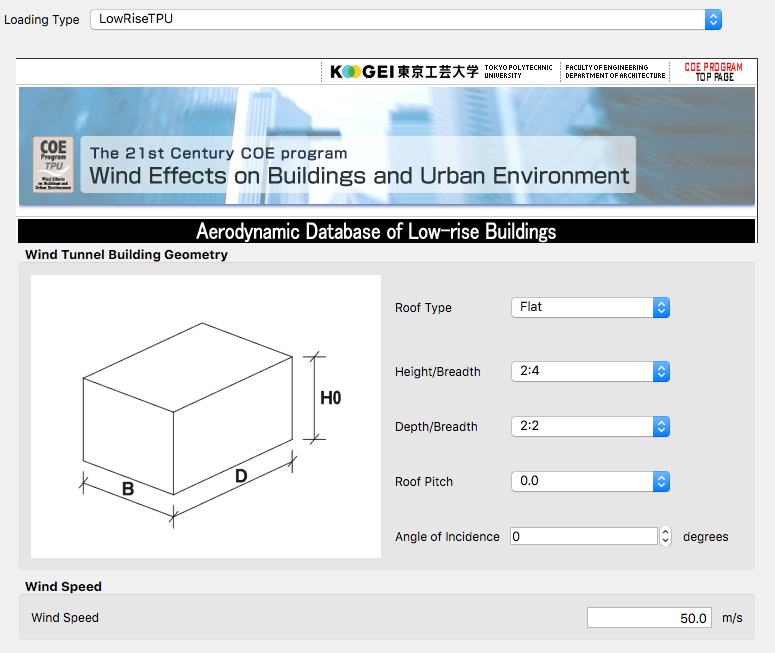
\includegraphics[width=0.8\textwidth]
    {usage/figures/lowRiseTPU.png} }
  \caption{Low Rise TPU Wind Loading Event}
  \label{fig:lowRiseTPU}
\end{figure}

In the inputs for the event, as shown in figure \Cref{fig:lowRiseTPU} require the user to specify which 
of these tests to use:
\begin{enumerate} 
\item The roof type, currently only flat is an option.
\item The user specifies one of 4 height to breadth ratios.
\item One of three depth to breadth ratios.
\item A roof picth.
\item The angle of incidence, 0 through 90 in 15 degree increments.
\item Mean Wind Speed: The wind speed provided is used in determing the velocity factor and the applied loads. 
\end{enumerate}

Random Variables: For this event, the wind speed can be a random variable.



\subsection{Wind Tunnel Experiment}
\label{subsec:windTunnelExperiment}
This application will take the wind tunnel data provided and scale it based on wind speed provided in this interface, and the building dimensions provided in the General Information. The theory on scaling wind tunnel data is provided in the theory. The data for the winnd tunnel is provided in a JSON file format. That file contains information on model dimensions, model wind speed, and model frequency, tap locations and time varying pressure tap coefficients.

\begin{figure}[!htbp]
  \centering {
    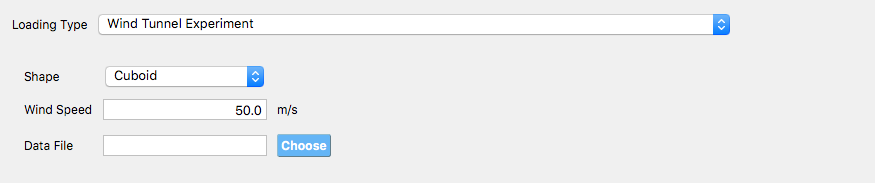
\includegraphics[width=0.8\textwidth]
    {usage/figures/windTunnelExperiment.png} }
  \caption{Wind Tunnel Experiment  Wind Loading Event}
  \label{fig:dedm_hrp}
\end{figure}

\begin{enumerate} 
\item The user to select the shape of the building, currently onlu Cuboid shapes are permitted.
\item The Wind Speed.
\item The file containing the experimental data. The file contains information about the dimensions of the building model in the wind tunnel, the wind speed (the meaning of wind speed dis totally dependent on what wind speed measurement was used in the test), time varying data for the pressure coeffiecients, information on frequency of these data points, and information on th elocations of pressure taps for which pressure coefficients are provided. An abbreviated example is as shown below.
\end{enumerate}


Random Variables: For this event, the wind speed can be a random variable.

The format for the wind tunnel data file is presently a JSON file. Future versions will allow the input of Matlab .mat files. A valid file is as follows:

\begin{verbatim}
{
 "meanWindSpeed":22.000000,
 "shape":"Cuboid",
 "depth":24.000000,
 "height":12.000000,
 "breadth":16.000000,
 "frequency":600.000000,
 "period": 15.000000,
  "units":{
     "length":"m",
     "time":"sec"
  },
  "tapLocations": [
       {"id":1,"xLoc":1.000000,"yLoc":15.000000,"face":5},
       {"id":2,"xLoc":3.000000,"yLoc":15.000000,"face":5},
       ......
  ],
 "pressureCoefficients": [
       {"id": 1 , "data":[-1.083194,-1.372954, ....]},
       {"id": 2 , "data":[-1.181435,-1.164351, ....]},
       ......
   ]
}
\end{verbatim}

It should be noted that at present the only valid shape is a Cuboid. Other shapes for example representing low-rise buildings with different roof shapes will be available in future versons.

For a cuboid the input file contains information about the wind tunnel models width, depth, height and wind speed. In addition for each of the 5 faces the user provides information on tap location for which pressure coefficents are given. The coordinate system for each face is x and ym and assumes the origin is at bottom left of an elevation of the building assuming user is looking at that face of the building, as shown in figure.






\subsection{Existing}
\label{subsec:multiple_existing}
This panel is provided for the user to specify multiple existing SimCenter
event files.  If more than one event is specified it is done to
provide the UQ engine with a discrete set of events to choose
from\textemdash it is not done with the intention of specifying that
one event follows another.  The panel presented to the user
is shown in \Cref{fig:SC_event_panel}.

\begin{figure}[!htbp]
  \centering {
    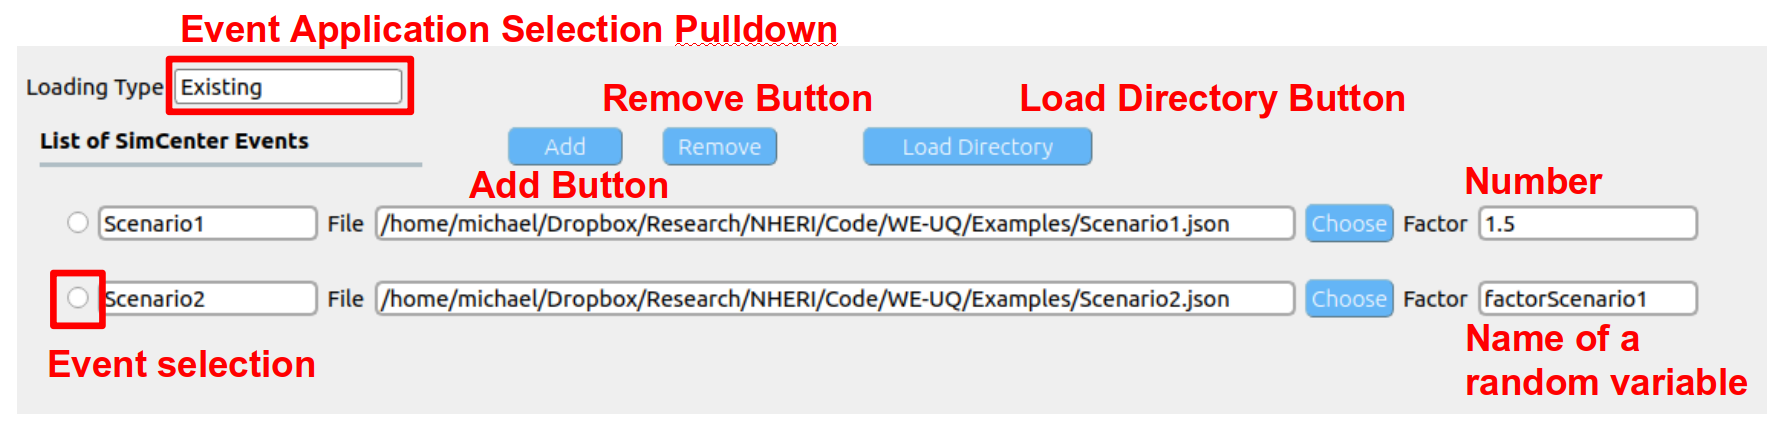
\includegraphics[width=0.8\textwidth]
    {usage/figures/weuqExisting.png} }
  \caption{Existing (SimCenter) Events }
  \label{fig:SC_event_panel}
\end{figure}

Use the \texttt{Add} button to add a new event. This adds an empty
event to the panel. Pressing the button multiple times will keep
adding events to the panel. \Cref{fig:SC_event_panel} shows the state
after the button has been pressed twice, and data entered to load
the \texttt{Scenario1} and \texttt{Scenario2} Events.

The path to the event file can be entered manually, or using
the \texttt{Choose} button for convenience. Pushing the button brings
up a typical file search screen. By default, a scale factor of 1.0 is
assigned to the event.  The user can change this to another floating
point value (DO NOT USE INTEGER), and they can define the scale factor
as a random variable by entering a variable name, such
as \texttt{factorScenario1} for the second event
in \Cref{fig:SC_event_panel}.

Note: the name of the random variable must not start with a number, or
contain any spaces or special characters, such as -, +, \%, etc.

The \texttt{Remove} button is used to remove events. To remove an
event, the user must first select events they wish to remove, which is
done by clicking in the small circle at the left side of the event
frame. All of the selected events are removed when the \texttt{Remove}
button is pressed.

The \texttt{Load Directory} button provides a convenient method to
load multiple events. All event files shall first be placed into the
same folder. We recommend to put the files in a folder of their own,
with no other files besides the wind loading events in it. After
pressing the \texttt{Load Directory} button, the user will be able to
choose the directory that contains the files, and the application will
load all event files (i.e., every file with a \texttt{.json}
extension) into the widget automatically.

Initially, every event will be given a load factor of 1.0. Load
factors can be assigned automatically by preparing
a \texttt{Records.txt} file in the directory with the events. Each
line in the \texttt{Records.txt} shall represent one event file, and
contain two comma separated values: the event file name and the
desired scale factor. The application will open that file
automatically and assign the prescribed load factors to the
events. Using a \texttt{Records.txt} file also allows users to load
only a subset of the events from a folder by listing only those in the
file. An example \texttt{Records.txt} is shown below:

\begin{verbatim}
Scenario1.json,1.5
Scenario2.json,2.0
\end{verbatim}

Random Variables: Scale factors can be defined as being random
variables by entering a string in the factor field. The variable name
entered will appear as a Random Variable in the UQ panel and the user
must specify its distribution there. If multiple events are specified,
the event itself will be also be treated as a random variable, with
each event being part of the discrete set of possible events. For this
discrete set the user does not define a distribution as this is done
automatically.


}{ 
\label{sec:event}
The event panel presents the user with a drop-down menu with a list of
available event applications. Event applications are applications
that, given the building and user supplied data inputs, will generate
a list of events (i.e., typically time-dependent loads that represent natural disasters) for the building. The following options
are available in the drop-down menu:

\begin{enumerate}
\item Multiple Existing SimCenter Events (\Cref{subsec:multiple_existing})
\item Multiple PEER Events (\Cref{subsec:multiple_peer})
\item Hazard Based Event (\Cref{subsec:hazard_based})
\item Stochastic Ground Motion (\Cref{subsec:stochastic_motions})
\item Site Response (\Cref{subsec:site_response})
\item User Application (\Cref{subsec:user_event})
\end{enumerate}

\subsection{Multiple Existing}
\label{subsec:multiple_existing}
This panel is provided for the user to specify multiple existing SimCenter
event files.  If more than one event is specified it is done to
provide the UQ engine with a discrete set of events to choose
from\textemdash it is not done with the intention of specifying that
one event follows another.  The panel presented to the user
is shown in \Cref{fig:SC_event_panel}.

\begin{figure}[!htbp]
  \centering {
    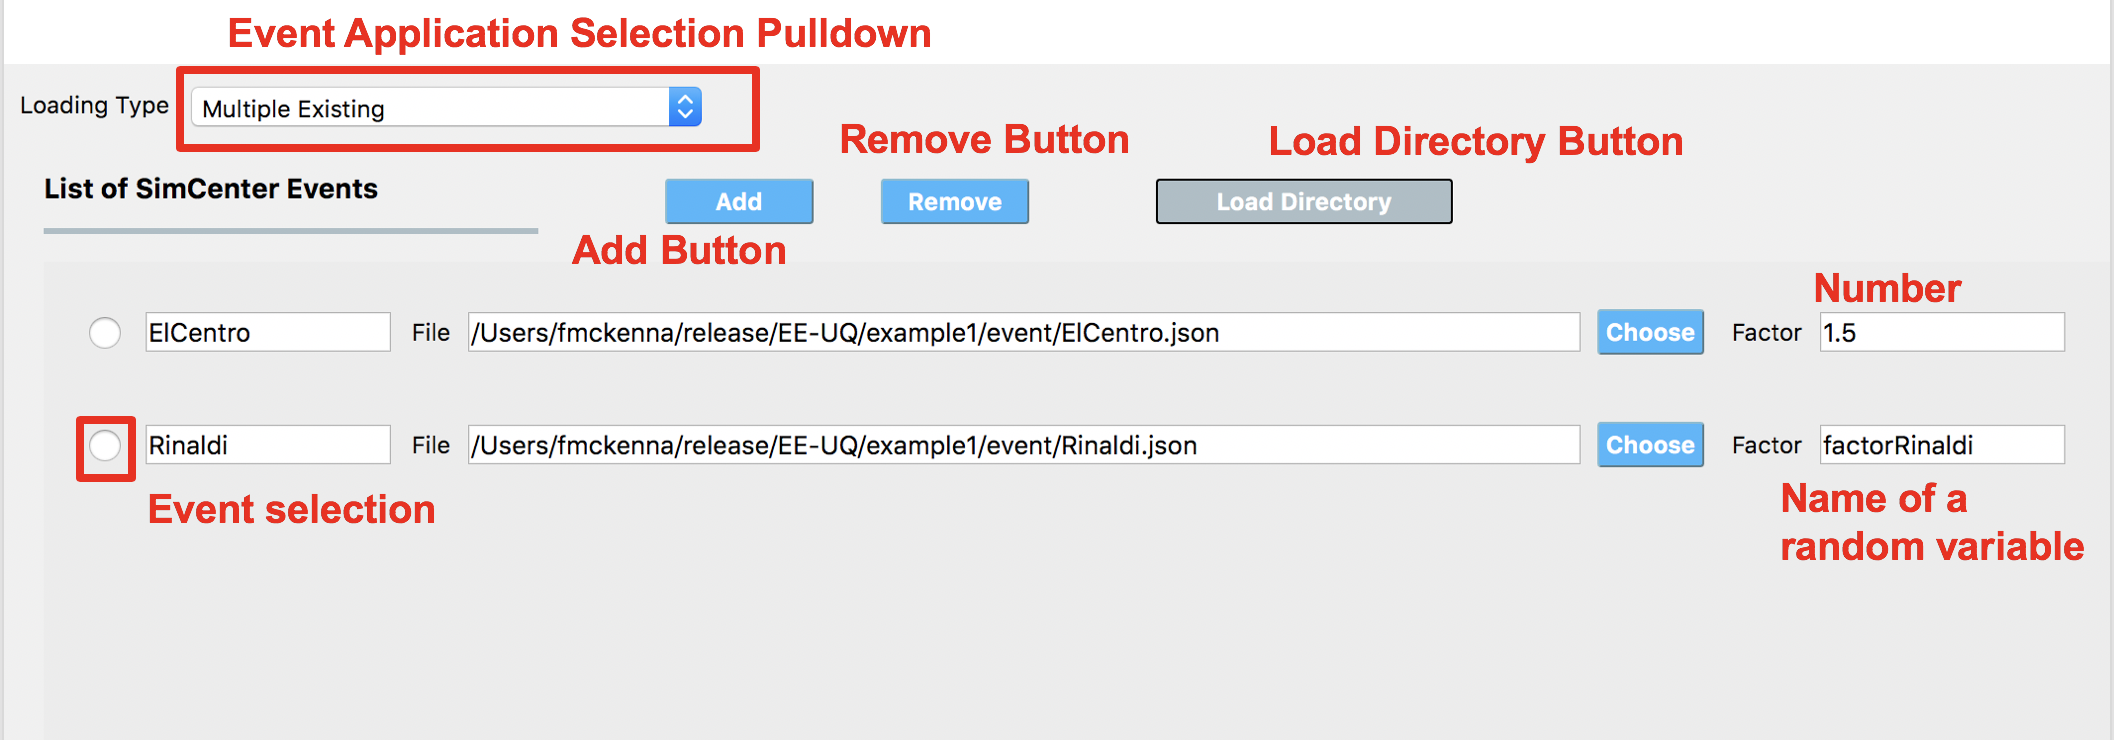
\includegraphics[width=0.8\textwidth]
    {usage/figures/multipleExisting.png} }
  \caption{Multiple Existing (SimCenter) Events }
  \label{fig:SC_event_panel}
\end{figure}

Use the \texttt{Add} button to add a new event. This adds an empty
event to the panel. Pressing the button multiple times will keep
adding events to the panel. \Cref{fig:SC_event_panel} shows the state after
the button has been pressed twice, and data entered to load the El Centro
and Rinaldi Events.

The path to the event file can be entered manually, or using the \texttt{Choose} button for convenience. Pushing the button brings up a typical file search screen. By default, a scale factor of 1.0 is assigned to the event.  The user
can change this to another floating point value (DO NOT USE INTEGER), and they can define the scale factor as a random variable by
entering a variable name, such as \texttt{factorRinaldi} for the second event in \Cref{fig:SC_event_panel}.

Note: the name of the random variable must not start with a number, or contain any spaces or special characters, such as -, +, \%, etc.

The \texttt{Remove} button is used to remove events. To remove an
event, the user must first select events they wish to remove,
which is done by clicking in the small circle at the left side of the event frame. All of the selected events are removed when the \texttt{Remove} button is pressed.

The \texttt{Load Directory} button provides a convenient method to load multiple events. All event files shall first
be placed into the same folder. We recommend to put the files in a folder of their own, with no other files besides the earthquake events in it. After pressing the \texttt{Load Directory} button, the user will be able to choose the directory that contains the files, and the
application will load all event files (i.e., every file with a \texttt{.json} 
extension) into the widget automatically. 

Initially, every
event will be given a load factor of 1.0. Load factors can be assigned automatically by preparing a \texttt{Records.txt} file in the directory with the events. Each line in the \texttt{Records.txt} shall represent one event file, and contain two comma separated values: the event file name and the desired scale factor. The application will open that file automatically and assign the prescribed load factors to the events. Using a \texttt{Records.txt} file also allows users to load only a subset of the events from a folder by listing only those in the file. An example \texttt{Records.txt} is shown below:

\begin{verbatim}
ElCentro.json,1.5
Rinaldi.json,2.0
\end{verbatim}

Random Variables: Scale factors can be defined as being random variables by entering a string in the factor field. The variable name entered will appear as a Random Variable in the UQ panel and the user must specify its distribution there. If multiple
events are specified, the event itself will be also be treated as a random
variable, with each event being part of the discrete set of possible
events. For this discrete set the user does not define a distribution as this is done automatically.


\subsection{Multiple PEER Event}
\label{subsec:multiple_peer}
This event option is provided for the user to specify multiple existing
\href{http://peer.berkeley.edu}{PEER} ground
motion files. PEER files contain time-histories in a single degree of freedom; hence, if multi-degree-of-freedom excitation is desired, the user is required to specify each
individual component for every EVENT. The \texttt{Add/Remove} buttons
at the top are to create and remove an event, as
per \Cref{subsec:multiple_existing}. The \texttt{+} and \texttt{-} buttons add and remove
components (see \Cref{fig:PEER_event_panel}). Remove removes all selected components. Each
component in a PEER event can have their own scale factor, which can be assigned a random variable.

\begin{figure}[!htbp]
  \centering {
    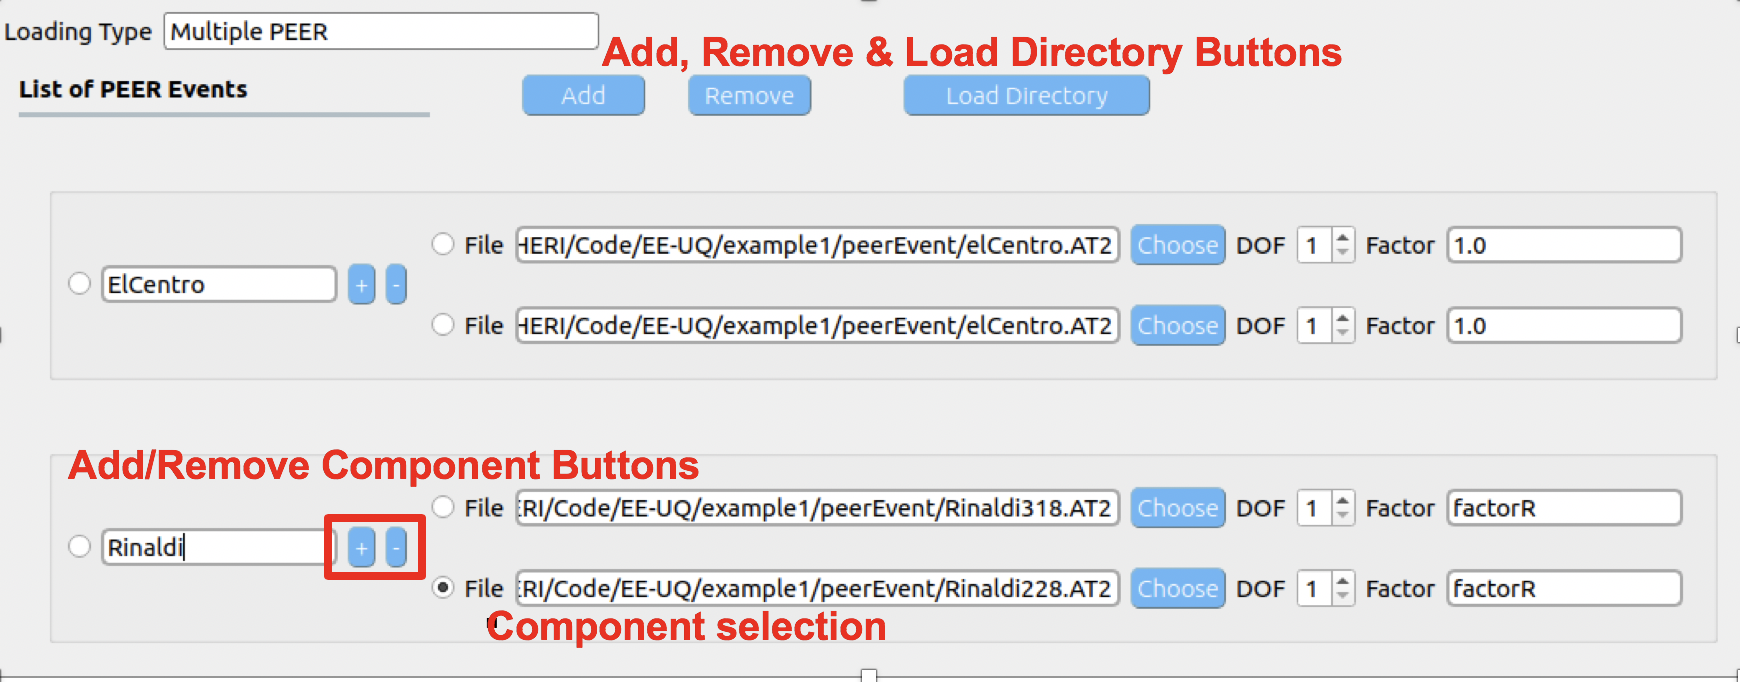
\includegraphics[width=0.8\textwidth]
    {usage/figures/multiplePEER.png} }
  \caption{Multiple PEER Events}
  \label{fig:PEER_event_panel}
\end{figure}

The \texttt{Load Directory} button and the \texttt{Records.txt} file works for PEER events as described in \Cref{subsec:multiple_existing}. The only difference is that PEER files are expected to have an \texttt{.AT2} extension. Only files with that extension shall be specified in the \texttt{Records.txt}.
An example \texttt{Records.txt} file for multiple Peer
events is shown below:

\begin{verbatim}
elCentro.AT2,1.5
Rinaldi228.AT2,2.0
Rinaldi318.AT2,2.0
\end{verbatim}

Random Variables: Random scale factors can be defined by entering a string in the factor field. The variable name entered will appear as a Random Variable in the UQ panel and the user must specify its properties there. If multiple
events are specified, the event itself will be treated as a random
variable, with each event being part of the discrete set of possible
events. For this discrete set the user does not define a distribution as this is done automatically bu the UI.


\subsection{Hazard Based Event}
\label{subsec:hazard_based}
The panel for this event application is as shown in
\Cref{fig:hazard_based_event_panel}. This application implements a scenario-based
(deterministic) seismic event.  In this panel the user specifies an
earthquake rupture (location, geometry and magnitude), a ground motion
prediction equation (GMPE), a record selection database and the intensity
measure used for record selection. In the backend, this application
relies on three other applications to perform seismic hazard analysis,
intensity measures simulation (to create a simulated target spectrum),
and ground motion record selection/scaling. Users interested in
learning about those applications are referred to the documentation of
the
\href{https://github.com/NHERI-SimCenter/GroundMotionUtilities/blob/master/Readme.md}{SimCenter
  Ground Motion Utilities}.

\begin{figure}[!htbp]
  \centering {
    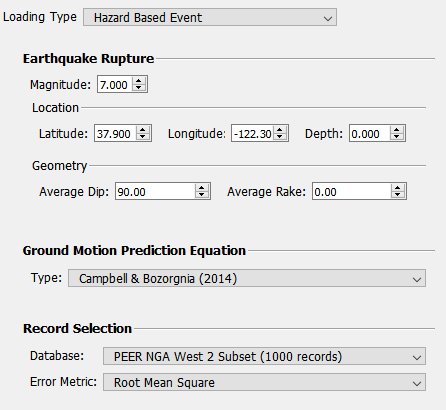
\includegraphics[width=0.5\textwidth]
    {usage/figures/hazardBased.png} }
  \caption{Hazard Based Event}
  \label{fig:hazard_based_event_panel}
\end{figure}


\subsection{Stochastic Ground Motion Model}
\label{subsec:stochastic_motions}
This option allows users to generate synthetic ground motions for a
target seismic event. In order to do so, the stochastic ground motion
model is selected from the drop-down menu, as shown
in \Cref{fig:stochastic_loading}. Depending on the model selected, the
user will be asked to enter values for a number of parameters that are
used to generate a seismic event. In the current release, users can
select between the model derived by Vlachos et
al. (2018) \cite{vlachos2018predictive} and the model developed by
Dabaghi \& Der Kiureghian (2014, 2017, 2018)
[\cite{dabaghi2014stochastic}, \cite{dabaghi2017stochastic}, \cite{dabaghi2018simulation}]. The
geometric directivity parameters, as shown in \Cref{fig:dabaghi}, required by the Dabaghi \& Der
Kiureghian model are described completely in Somerville et al. (1997)
\cite{somerville1997modification}. Additionally, users can provide a
seed for the stochastic motion generation if they desire the same
suite of synthetic motions to be generated on multiple occasions.  If
the seed is not specified, a different realization of the time history
will be generated for each run. The backend application that generates
the stochastic ground motions relies on \texttt{smelt}, a modular and
extensible C++ library for generating stochastic time histories. Users
interested in learning more about the implementation and design of
\texttt{smelt} are referred to its
\href{https://github.com/NHERI-SimCenter/smelt}{GitHub repository}.

All input parameters can be specified as random variables by entering
a string in the parameter field. Please note that information for the
inputs that are identified as random variables needs to be provided in
the \texttt{UQ} tab.

\begin{figure}[!htbp]
  \centering
    \begin{subfigure}{\textwidth}
        \centering
        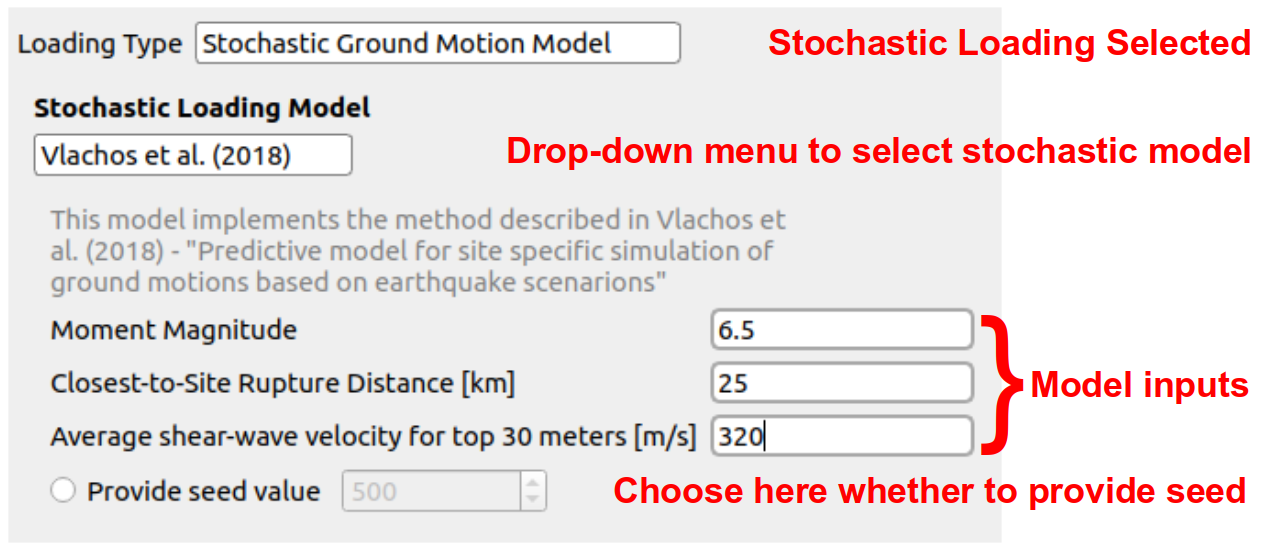
\includegraphics[width=\textwidth]{usage/figures/stochastic_loading.png}
        \caption{Vlachos et al. (2018) model inputs}
    \end{subfigure}
    \hspace*{\fill}
    
    \begin{subfigure}{\textwidth}
        \centering
        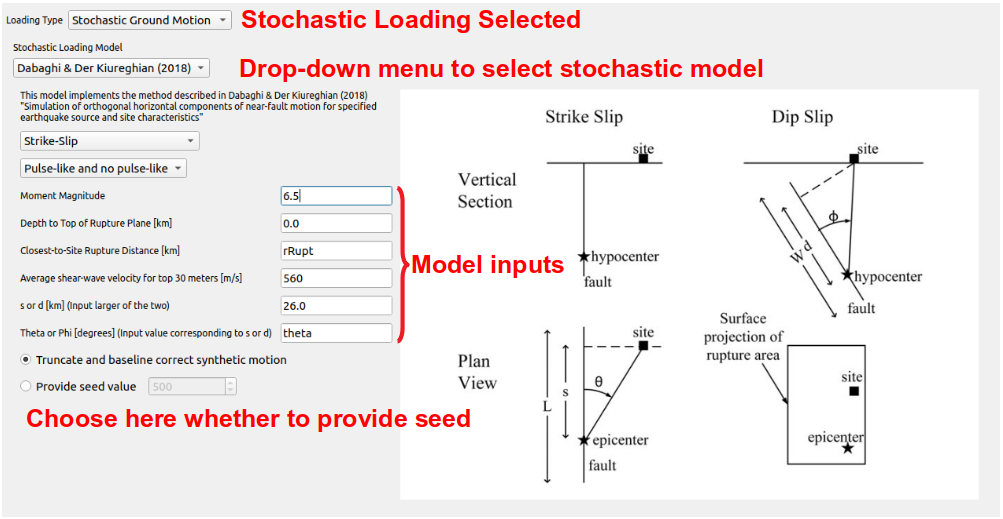
\includegraphics[width=\textwidth]{usage/figures/stochastic_dabaghi.png}
        \caption{Dabaghi \& Der Kiureghian (2018) model inputs}
        \label{fig:dabaghi}        
    \end{subfigure}
    
  \caption{Stochastic Ground Motion Event}
  \label{fig:stochastic_loading}    
\end{figure}


\subsection{Site Response}
\label{subsec:site_response}
This option allows users to determine the event at the base of the 
building by performing an effective free-field site response 
analysis of a soil column. In this panel the user specifies a ground 
motion at the bottom of the column. After the soil layers have been properly 
defined, the motion at the ground surface are given at the end 
of the analysis, and is is this motion will be used in the 
simulation of the building response. 

\begin{figure}[!htbp]
  \centering {
    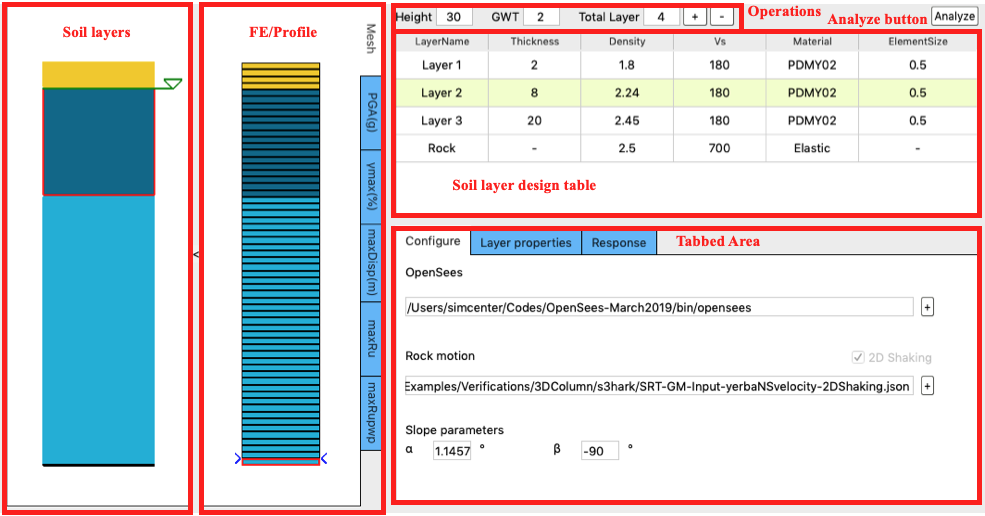
\includegraphics[width=0.8\textwidth]
    {usage/figures/s3hark1.png} }
  \caption{Site Response Analysis Event}
  \label{fig:s3hark1}
\end{figure}

The UI of the Site Response is shown in \Cref{fig:s3hark1}. It is split into the following areas:
\begin{enumerate}
\item Soil Column Graphic: The first graphic on the left of the panel shows a visualization of the soil column. To select a layer, the user must move their cursor over the area and then select it. The selected layer will be outlined with a red box.
\item FE Mesh Graphic: The second graphic on the left shows 
the finite element mesh and profile plots. Selecting any of the tabs on the right inside this graphic (i.e, PGA, $\gamma_{max}$, maxDisp, maxRu, maxRuPWP) will show various results
from the simulation at the mesh points.
\item Operations Area: The right side of this area shows the height, total number of soil layers, graound water table (GWT), and includes plus and minus buttons. 
If the user presses the plus button, a layer is added below the selected layer. If the minus button is pressed the selected layer is removed. The GWT input field allows the user to specify the level of the ground water table.
\item Analyze Button: A button the user presses when inputs for this widget are all entered. The site response tool currently requires the site response analysis is performed before the RUN button can be pressed.
\item Soil Layer Table: This table is where the user provides the characteristics of the soil layer, such as layer thickness, density, $V_{s30}$, material type, and element size in the finite element mesh.
\item Tabbed Area: This area contains the three tabbed widgets described below.

\begin{figure}[!htbp]
  \centering {
    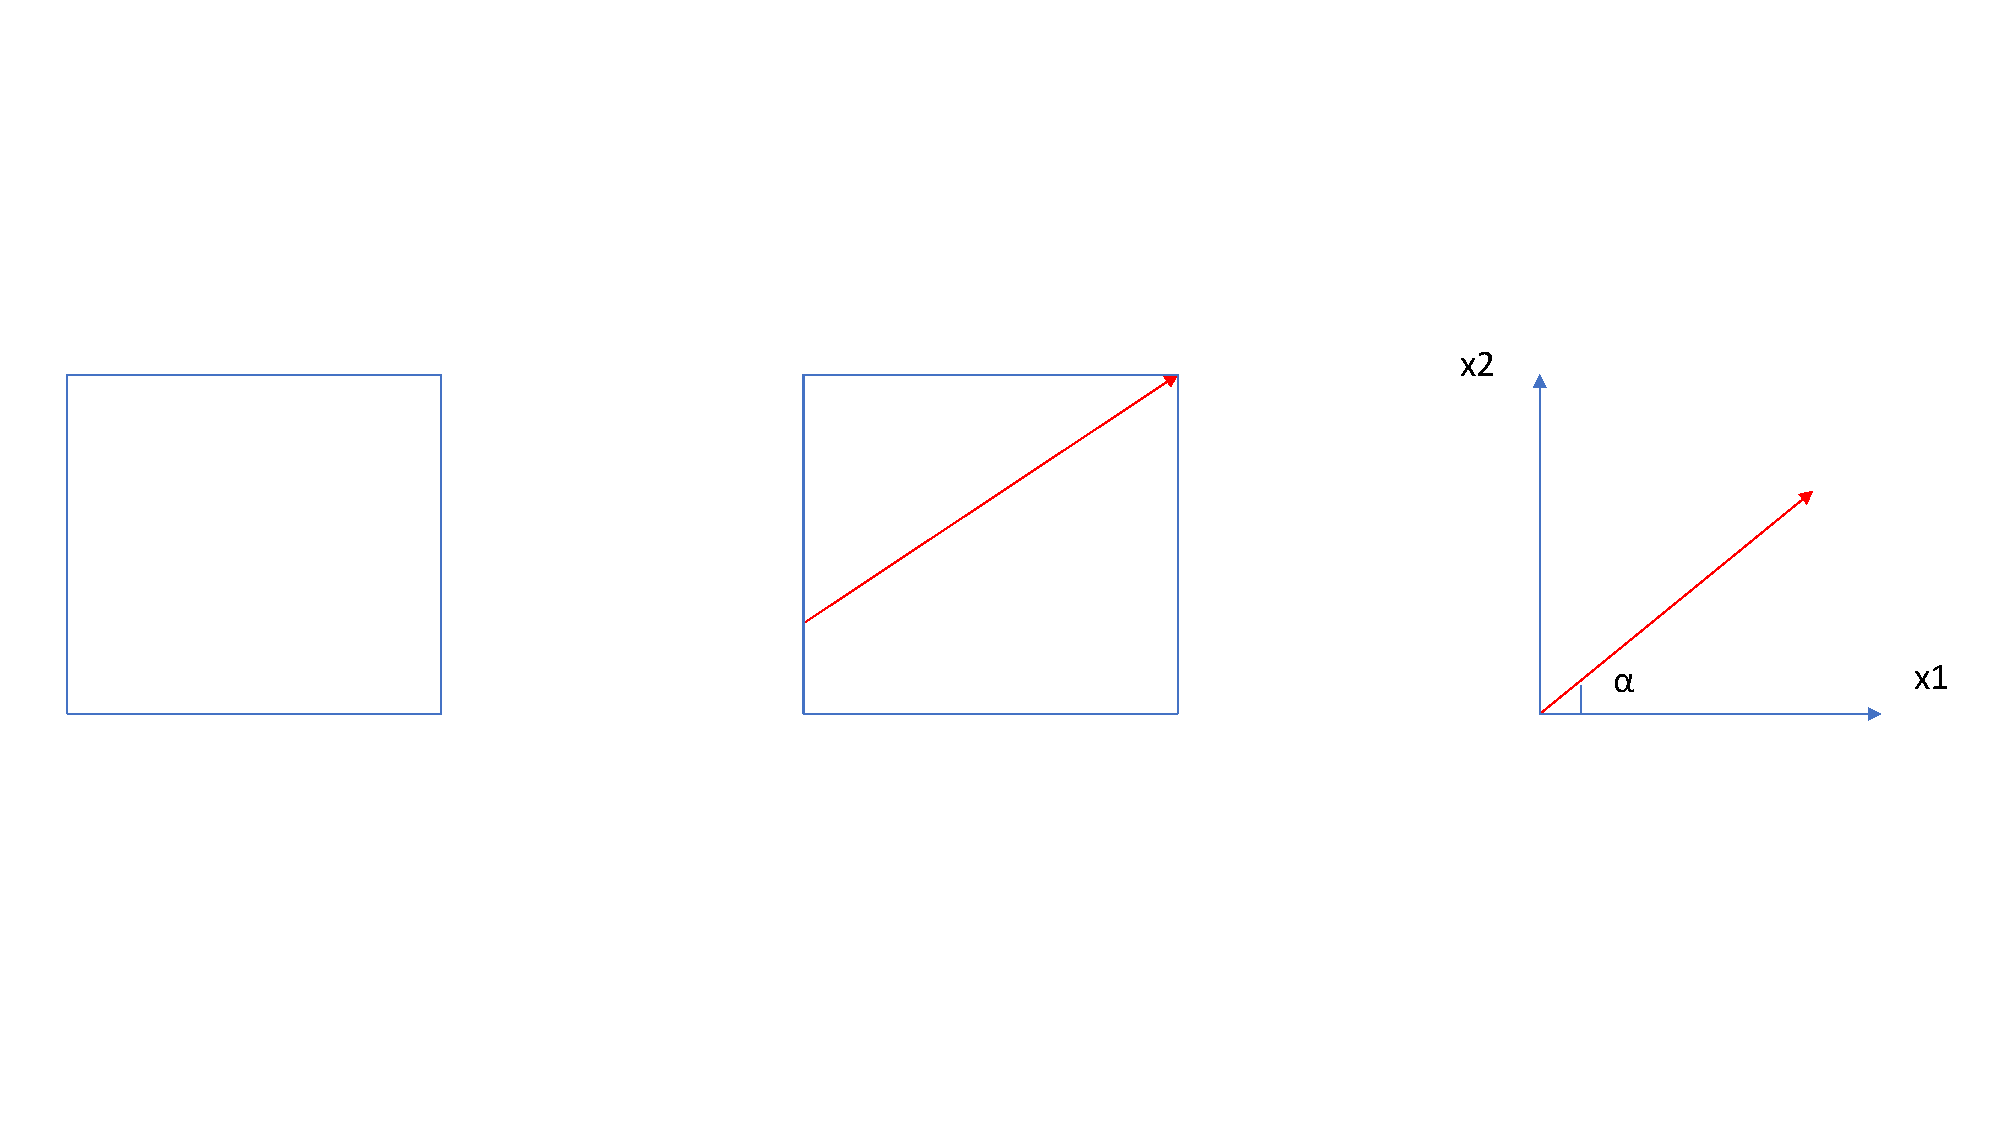
\includegraphics[width=0.8\textwidth]
    {usage/figures/2DSlope.pdf} }
  \caption{Slope definition for 2D Column }
  \label{fig:slope2D}
\end{figure}


\begin{figure}[!htbp]
  \centering {
    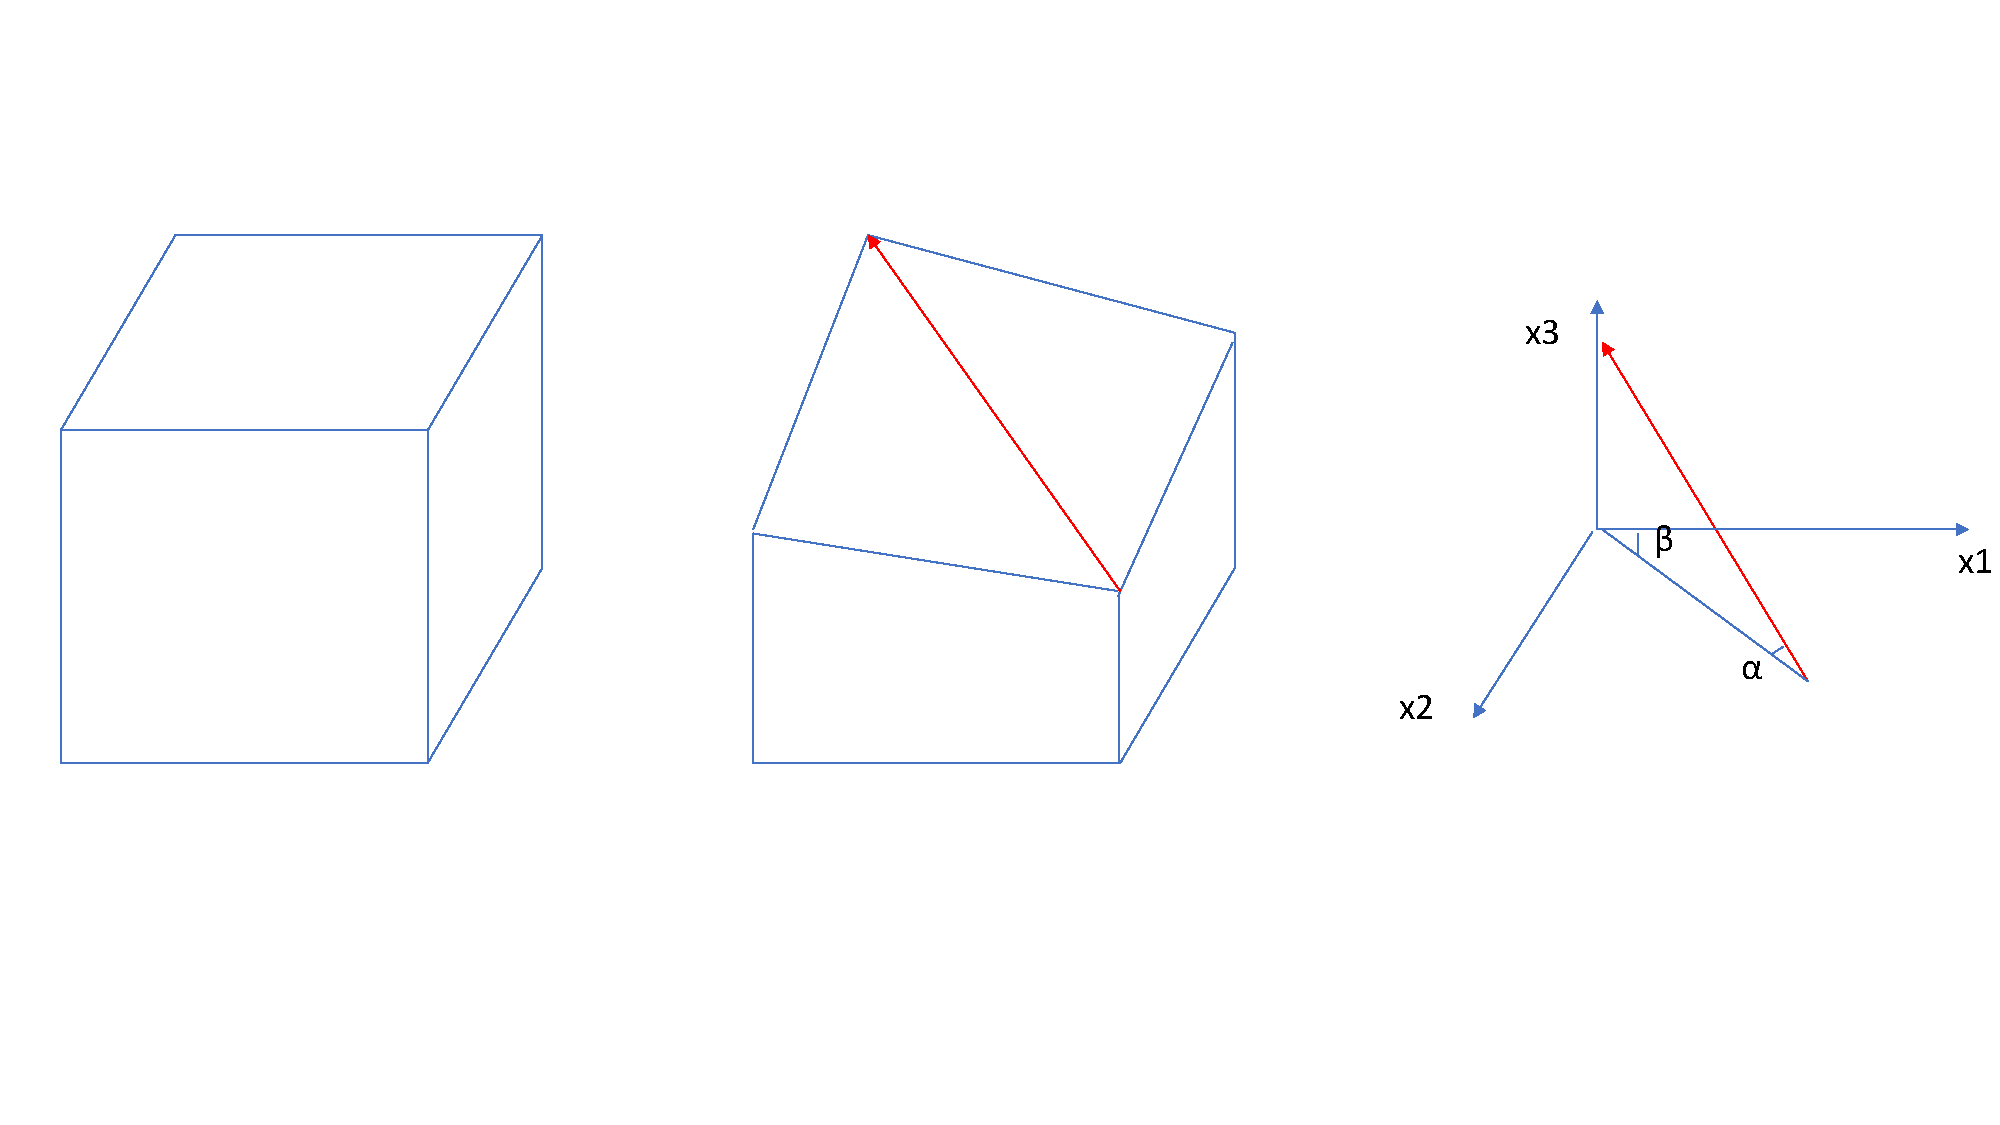
\includegraphics[width=0.8\textwidth]
    {usage/figures/3DSlope.pdf} }
  \caption{Slope definition for 3D Column}
  \label{fig:slope3D}
\end{figure}


\begin{figure}[!htbp]
  \centering {
    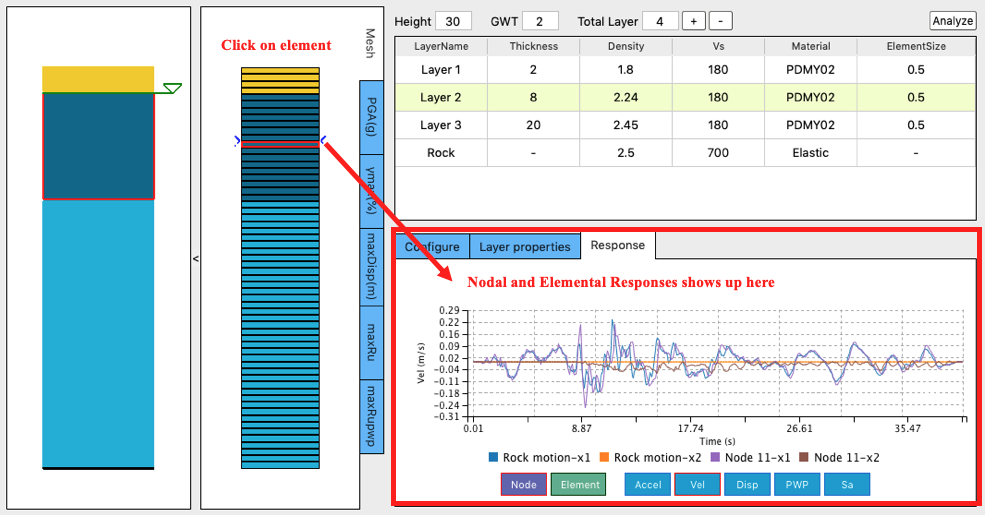
\includegraphics[width=0.8\textwidth]
    {usage/figures/response.png} }
  \caption{Nodal and elemental responses}
  \label{fig:response}
\end{figure}

\begin{enumerate}
  \item Configure Tab: This tab allows the user to specify the path to the OpenSees executable and to a ground motion file that represent the ground shaking at the bedrock. 
  The rock motion file must follow the SimCenter event format. Examples of SimCenter event files are available with the \href{https://github.com/NHERI-SimCenter/EE-UQ/tree/master/example1/event}{source code}.
  \textit{s$^3$hark}  will determine to use 2D column or 3D column based on the ground motion file provided.
  When a ground motion file is selected from the local computer, or the path of the ground motion file is typed in, \textit{s$^3$hark} will figure out if it's a 1D or 2D shaking file. 
  If it's 1D shaking, all elements will be 2D. If it's 2D shaking, all elements will be 3D. The definition of 2D and 3D slope are different. See \Cref{fig:slope2D} and \Cref{fig:slope3D}.
  \item Layer Properties Tab: This tab allows the user to enter additional material properties for the selected soil layer (\Cref{fig:s3hark3}).
  \item Response Tab: Once the site response analysis has been performed, this tab provides information about element and nodal time varying response quantities. See \Cref{fig:response}.
  \item Run Tab: Opens up a window in which by using the up and down arrows on the keyboard the dino will jump up and down. Something to do if the site response analysis is taking too long, which it may if many soil layers are used.
\end{enumerate}

\item Analyze Button: This button shall be used to run the simulation locally. A progress bar will show the status of the analysis. This allows the user to review the ground motion predicted at the surface.
\end{enumerate}

\begin{figure}[!htbp]
  \centering {
    \includegraphics[width=0.8\textwidth]
    {usage/figures/s3hark3.pdf} }
  \caption{Soil Layer Modification in Site Response }
  \label{fig:s3hark3}
\end{figure}

Upon the finish of the finite element analysis, the ground motion at the soil surface (\Cref{fig:s3hark4}) will be stored in EE-UQ's input file.
This computed motion will be applied during the simulation.

\begin{figure}[!htbp]
  \centering {
    \includegraphics[width=0.4\textwidth]
    {usage/figures/s3hark4.png} }
  \caption{Simulated Motion at the Surface of the Ground}
  \label{fig:s3hark4}
\end{figure}

Random Variables: The current version of the Site Response event type does not support random variables.\\

NOTES: 
\begin{enumerate}
\item Variables are assumed to have m, kPa, and kN units in the Site Response panel.
\item If the Analyze button is not pressed, no simulation will be performed. If no simulation is performed there will be no ground motions provided to the building.
\end{enumerate}


\subsection{User Application}
\label{subsec:user_event}
The final option for event definition is a user application. 
The user specifies the application name and the input file containing the specific input information 
needed by the application when it is running in the backend. 
As will be discussed later, is the user selects to utilize an application that is not provided, they are also required to edit the tools registry file. Here they must include a new event application with the same name as that entered and they must provide the location where that application can be found relative to the tools application directory. 
If running on DesignSafe, that application must be built and must be available on the Stampede2 supercomputer. 

Note: Given how DesignSafe runs the applications through Agave, the file permissions of this application must be world readable and executable.

\begin{figure}[!htbp]
  \centering {
    \includegraphics[width=1.0\textwidth]
    {usage/figures/userAppEvent.png} }
  \caption{User defined event}
  \label{fig:user_defined_event_panel}
\end{figure}


\subsection{PEER NGA Records}
\label{subsec:peer_nga_records}


This event allows the user to perform ground motion records selection and scaling using PEER NGA West 2 ground motions database. The suite of records can be selected from the database to represent the uncertainty in the ground motion. The following steps are needed to use this event:


\enumerate{
\item A target response spectrum must be specified by the user to be used for records selection and scaling.
\item The user specifies a selection criteria, such as the number of records and optional ranges of earthquake magnitude, distance to rupture (R\textsubscript{rup}) and shear wave velocity in the top 30 meter of soil (V\textsubscript{s}30).
\item The user run the record selection and inspect the selected suite of ground motions.
}


It is important to note that this event requires a PEER NGA West 2 account, users will be asked to provide their credentials (user name and password) to log in to the database. Users who do not have an account will be forwarded to the account sign up web page. Record selection is always done to minimize the mean square error between the target spectrum and the selected scaled spectrum. It is also important to note that the current version only allows user to specify the ASCE 7-10 design spectrum as a target. Future versions will allow the users to specify a user-provided target spectrum or a target spectrum obtained from seismic hazard analysis, such as the uniform hazard spectrum (UHS) or the conditional mean spectrum (CMS).


\begin{figure}[!htbp]
  \centering {
    \includegraphics[width=0.8\textwidth]
    {usage/figures/PeerNgaRecords.png} }
  \caption{PEER NGA Records Event}
  \label{fig:PeerNgaRecordsWidget}
\end{figure}


After a suite of records is selected from the database, the list of records is shown in tabular form for the user to inspect their information, as shown in \Cref{fig:PeerNgaRecordsWidget}. Additionally a plot is generated showing the target spectrum, the average and standard deviation of the selected suite of records and the selected scaled ground motions spectra. Users can also highlight particular spectra on the plot by selecting the one or more records in the table provided. This enables the user to inspect the suite of records used to characterize the ground motions before running the building simulation.
}


\section{FEM: Finite Element Method}
\label{sec:fem}
The FEM panel will present users with a selection of FEM
applications that will take a building model generated by the BIM
application and the EVENT from the event application and perform a
deterministic simulation of structural response. Currently, there is one application
available, OpenSees, and there is no application selection box. That
will be modified in future versions to allow users to provide their own
simulation application. The current OpenSees implementation extends the standard OpenSees executable with a pre- and post-processor to take the BIM and EVENT
files and use OpenSees to simulate the response, and return it in an EDP file.

\begin{figure}[!htbp]
  \centering {
    \includegraphics[width=0.5\textwidth]
    {usage/figures/fem.png} }
  \caption{Options for \texttt{OpenSees} transient analysis}
  \label{fig:fem}
\end{figure}

For the OpenSees application the user is required to specify the
options to be used in the transient analysis. As shown in \Cref{fig:fem},
this includes the choice of
\begin{enumerate}
\item \href{http://opensees.berkeley.edu/wiki/index.php/Algorithm_Command}{Solution algorithm}, the default is Newton Raphson.
\item \href{http://opensees.berkeley.edu/wiki/index.php/Integrator_Command}{Integration Scheme}, the default is Newmark's linear acceleration
  method.
\item \href{http://opensees.berkeley.edu/wiki/index.php/Test_Command}{Convergence Test}, the default is a norm on the unbalance force.
\item Convergence tolerance, with a default of 0.01.
\item Damping Ratio. the default is 2\% equivalent viscous damping entered as 0.02. If
a damping ratio of 0 is specified, no damping is added by the simulation application. This allows users to add their own damping in the OpenSees tcl script they load under SIM.
\item Analysis Script. This shall be left blank by default. Advanced users of OpenSees who have their preferred analysis script
and wish to provide their own damping model can provide it here.
\end{enumerate}


The options available for each setting can be found in the OpenSees online user
manual.\\

A default transient analysis script is run with these inputs. It is
built for Version 3.0.0+ of OpenSees and uses a divide and conquer
algorithm to overcome convergence issues. This new algorithm
does not work for every nonlinear problem. The actual analysis command
that is created based on the defaults is the following:

\begin{verbatim}
numberer RCM
system Umfpack
integrator Newmark 0.5 0.25
test NormUnbalance 0.01 20 
algorithm Newton
analysis Transient -numSubLevels 2 -numSubSteps 10 
analyze $numStep $dt
\end{verbatim}

If the user specifies their own analysis script to run
instead of the default, they can take advantage of the \texttt{numStep} and \texttt{dt} variables that
are obtained from the EVENT and are automatically set by the program.


\section{UQ: Uncertainty Quantification}
\label{sec:uq}
Throughout the input specification the user is defining variables. As
described in the above sections many of these variables can be
specified by the user to be random variables. The UQ panel is where the user specifies the distribution of these random variables. Besides the properties of random variables, the sampling method and the number of requested samples shall also be defined by the user. The panel is split, as shown
in \Cref{fig:uq_panel}, into two frames:

\begin{enumerate}
\item Sampling Methods 
\item Random Variables
\end{enumerate}

\begin{figure}[!htbp]
  \centering {
    \includegraphics[width=0.8\textwidth]
    {usage/figures/uq1.png} }
  \caption{Uncertainty Quantification input panel}
  \label{fig:uq_panel}
\end{figure}

\subsection{Sampling Methods}
\input{usage/uq_forwardPropagationMethods}

\subsection{Random Variables}
The RV panel allows the user to specify the probabilistic distribution for the random problem at hand. The following probabilistic distributions for the random variables are currently supported: 

\begin{enumerate}
\item \href{https://dakota.sandia.gov//sites/default/files/docs/6.9/html-ref/variables-normal_uncertain.html}{Gaussian}
\item \href{https://dakota.sandia.gov//sites/default/files/docs/6.9/html-ref/variables-lognormal_uncertain.html}{Lognormal}
\item \href{https://dakota.sandia.gov//sites/default/files/docs/6.9/html-ref/variables-beta_uncertain.html}{Beta}
\item \href{https://dakota.sandia.gov//sites/default/files/docs/6.9/html-ref/variables-uniform_uncertain.html}{Uniform}
\item \href{https://dakota.sandia.gov//sites/default/files/docs/6.9/html-ref/variables-weibull_uncertain.html}{Weibull}
\item \href{https://dakota.sandia.gov//sites/default/files/docs/6.9/html-ref/variables-gumbel_uncertain.html}{Gumbel}
\end{enumerate} 


Each distribution has different parameters, and the user needs to select accordingly the parameters for the distribution selected for each random variable. Once the user selects the distribution of the random variable, the
corresponding input boxes for the parameters will show. 

\Cref{fig:rv} shows the panel for a problem with four Random Variables with all random input following Gaussian distributions. 

\begin{figure}[!htbp]
  \centering {
    \includegraphics[width=0.8\textwidth]
    {examples/fig_quofem/rv.png} }
  \caption{Random Variable specification}
  \label{fig:rv}
\end{figure}





\softwareSwitch{PBE}{
\section{DL: Damage and Loss Model}
\label{sec:dl}
The Damage and Loss panel provides users a convenient way to define the damage and loss model for the building. The dropdown list at the top of the panel allows users to choose between two loss-assessment methods: FEMA P58 \cite{applied_technology_council_atc_fema_2012} and HAZUS MH \cite{federal_emergency_management_agency_fema_hazus_2018-2}. The method chosen determines the information displayed in the rest of the panel. The two methods are discussed in the following sections.

\subsection{FEMA P58}

This option implements the loss assessment methodology described in the \href{https://www.fema.gov/media-library/assets/documents/90380}{FEMA P58} documents. The main panel is divided into four parts that can be accessed by clicking at the tabs at the top of the input panel.

\subsubsection{General Settings}

\Cref{fig:dl_p58_general} shows the first panel, which corresponds to general damage and loss settings. The panel allows the user to set the response, damage, and loss models for the assessment.

\begin{figure}[!htbp]
  \centering {
    \includegraphics[width=0.9\textwidth]
    {usage/figures/dl_p58_general.png} }
  \caption{The General Damage and Loss Settings panel. (The settings shown in the Figure serve demonstration purposes and are not the suggested inputs.)}
  \label{fig:dl_p58_general}
\end{figure}

\textbf{Response Model:}

\begin{itemize}
	\item Response Description:
	\begin{itemize}
		\item EDP data: Allows you to provide externally calculated EDP results for the assessment. If this field is not empty, we will use the raw results in the file provided and we will not run any response simulations regardless of the settings in other parts of the application. 
		\item EDP distribution: Specifies the approach to describing the distribution of EDPs. If empirical is selected, the raw EDPs are kept as is and resampled during the assessment. The lognormal setting fits a multivariate lognormal distribution to the EDPs. The truncated lognormal setting can be used to set a truncated multivariate lognormal distribution to the non-collapse results by setting the Basis (the next setting) appropriately.
		\item Basis: Specifies the basis of the EDP distribution. The all results setting uses all samples, while the non-collapse results removes the samples that have EDPs beyond the collapse limits (see in a later setting).
		\item Realizations: The number of EDP and corresponding damage and loss realizations to generate. Depending on the complexity of the model, a few thousand realizations might be sufficient to capture central tendencies. A much larger number is required to get appropriate estimates of the dispersion of results. If the EDP distribution is set to empirical, the EDP realizations are sampled from the set of raw EDP values with replacement. If the EDP distribution is set to lognormal or truncated lognormal, the samples are generated from the distribution that is fit to the raw EDP values.
	\end{itemize}
	\item Additional Uncertainty: Ground motion and Model uncertainty per FEMA P58. The prescribed logarithmic standard deviation values are added to the dispersion of EDPs to arrive at the description of uncertain building response.
	\item Detection Limits: These limits correspond to the maximum possible values that the response history analysis can provide. While peak interstory drifts will certainly have an upper limit, peak floor acceleration will not necessarily require such a setting. Leaving any of the fields empty corresponds to unlimited confidence in the simulation results.\\
	Note: these limits will be used to consider EDP data as a set of censored samples when fitting the multivariate distribution set under Response Description. If the EDP distribution is set to empirical, this setting has no effect.
\end{itemize}

\textbf{Damage Model:}

\begin{itemize}
	\item Irrepairable Residual Drift: Describes the limiting residual drift as a random variable with a lognormal distribution. See Figure 2-5 and Section 7.6 in FEMA P58 for details. The prescribed yield drift ratio is used to estimate residual drifts from peak interstory drifts per Section 5.4 in FEMA P58. This is only needed if no reliable residual drifts are available from the simulation. Considering the large uncertainty in estimated residual drift values, it is recommended to consider using the peak interstory drift as a proxy even if it would be numerically possible to obtain residual drift values.
	\item Collapse Probability: 
	\begin{itemize}
		\item Approach: Specifies if the collapse probability shall be estimated from EDP samples, or prescribed by the user.
		\item Prescribed value: If the prescribed approach is selected above, you can specify the probability of collapse here.
		\item Basis: If the estimated approach is selected above, you can specify the basis of collapse probability estimation here. Sampled EDP corresponds to using the (re)sampled EDPs, while raw EDP corresponds to using the EDP inputs to evaluate the proportion above the collapse limits to get the collapse probability.
	\end{itemize}
	\item Collapse Limits: If the Approach under Collapse Probability is set to estimated, the collapse of the building in each realization is inferred from the magnitude of EDPs. The collapse limits describe the EDP value beyond which the building is considered collapsed. Note that collapse limits might be beyond the detection limits (although that is generally not a good idea) and certain EDPs might not have collapse limits associated with them (e.g. PFA).
\end{itemize}

\textbf{Loss Model:}

\begin{itemize}
	\item Replacement Cost and Time: The cost (in the currency used to describe repair costs, typically US dollars) and the time (in days) it takes to replace the building.
	\item Decision variables of interest: These checkboxes allow the user to pick the decision variables of interest and save computation time and storage space by only focusing on those.
	\item Inhabitants:
	\begin{itemize}
		\item Occupancy Type: The type of occupancy is used to describe the temporal distribution of the inhabitants. Note: the default FEMA P58 distribution can be overridden by a custom file provided in the Custom Data Sources box.
		\item Peak Population: The maximum number of people present at each floor of the building. The example in \Cref{fig:dl_p58_general} shows a two-story wooden house with a cripple wall, hence the 0 population in the first floor.
		\item Custom distribution: The loss assessment is performed using population and fragility data from the first edition of FEMA P58. Each data source can be overridden by custom user-defined data.\\
		Note: the loss calculations are performed at the local computer. Consequently, the locally available fragility and population data files can be used to perform the calculations even if the response simulations are done at DesignSafe.
	\end{itemize}
\end{itemize}

\subsubsection{Building Components}

\Cref{fig:dl_p58_comp} shows the input panel where you can define the components of the building. 

The available components are from the second edition of FEMA P58 by default. The corresponding json files are available in the applications folder under: 

\texttt{performDL/pelicun/pelicunPBE/resources/FEMA P58 second edition/DL json/} 

The components from the first edition of FEMA P58 are also provided with the PBE app  under the \texttt{FEMA P58 first edition} folder at the above location. Typically, you will have to edit the components provided by FEMA P58 and specify fragility and consequence data before they can be used for damage and loss assessment. We recommend that you copy the components you prefer to use for the assessment to another folder and perform the edits there. Then, specify that folder under the Damage and Loss Data Folder field and PBE will automatically load those components and make them available for use.

\begin{figure}[!htbp]
	\centering {
		\includegraphics[width=0.9\textwidth]
		{usage/figures/dl_p58_comp.png} }
	\caption{The Component Settings panel. (The settings shown in the Figure serve demonstration purposes and are not the suggested inputs.)}
	\label{fig:dl_p58_comp}
\end{figure}

The \emph{Add Selected}, \emph{Add All}, \emph{Remove Selected}, \emph{Remove All} buttons allow you to Add or Remove components from the available set to the selected one. Only the selected components will be used during the loss assessment.

The \emph{Component Details} below provides more information about the active component in the drop-down menu under Selected components and allows you to specify where and what quantities of those components are in the building. Components are handled by defining component groups in the building. You can add a new component group definition or remove and existing one with the \emph{Add Component Group} and emph{Remove Component Group} buttons. Each component group defintion allows you to assign component groups to various locations in the building. The following settings are available:

\begin{itemize}
	\item location(s): In buildings, locations are typically stories. The ground floor is story 1. Providing 'all' assigns the same setting to every story. You can use a dash to specify a range of stories, such as '3-7'. If a component is only assigned to the top story, or the roof, you can use 'top' or 'roof'. You can also combine these and use '3-roof' for example. These settings make it easy to transfer performance models between buildings that have a different number of stories.
	\item direction: The directions correspond to EDPs that are used to assess the fragility of the components. They shall match the directions in the EDP results available from the simulations.
	\item median quantity: Components within a Fragility Group are separated into Performance Groups by floor and direction. Components within a Performance Group are further separated into Component Groups that might experience independent damage and losses depending on the settings in the General tab. The list of quantities provided here specifies the number of Component Groups in each Performance Group that is created by this row.
	\item unit: The unit you used to specify component quantities. The default unit from the fragility database is provided among the component details above for convenience. As long as the unit belongs to the same class (i.e., length, area, etc.), you can use any of the commonly used metric or US units. Squared units are expressed by using a '2' after the name, such as 'ft2' for square feet.
	\item distribution: If you want to model the uncertainty in component quantities, select either normal or lognormal distribution here. The 'N/A' setting corresponds to known quantities with no uncertainty.
	\item cov: Coefficient of variation for the random distribution of component quantities. If the distribution is set to 'N/A', this can be left blank.
\end{itemize}

As long as you want to assign the same amount of components to every floor and every direction, one component group definition is sufficient. Oftentimes, you will want to have more control over component quantities. For example, in \Cref{fig:dl_p58_comp}, we assigned two groups with two braces in each group to the first and second floor in direction 1, and three groups with two braces in each to all floors in direction 2.

You can save the assigned performance model using the \emph{Save Performance Model to CSV} button. The created csv file can be loaded by Excel or Matlab allowing you to edit it and reuse it later. If you have a pre-defined performance model available in a csv file, you can load it with the \emph{Load Performance Model from CSV}. Make sure you have the Data Folder with the fragility definitions properly set up before loading a file that uses non-default components.

\subsubsection{Collapse Modes}

\Cref{fig:dl_p58_collmod} shows the input panel where you can specify the collapse modes of the building. Collapse modes provide information for the estimation of injuries from building collapse. As such, they are only used if injuries are among the requested Decision Variables. The following pieces of information are required for each collapse mode:

\begin{figure}[!htbp]
  \centering {
    \includegraphics[width=0.9\textwidth]
    {usage/figures/dl_p58_collmod.png} }
  \caption{The Collapse Modes panel. (The settings shown in the Figure serve demonstration purposes and are not the suggested inputs.)}
  \label{fig:dl_p58_collmod}
\end{figure}

\begin{itemize}
    \item name: A name that helps you identify the collapse mode. It is arbitrary and not used by the loss assessment engine.
    \item probability: Conditioned on collapse, the likelihood of this collapse mode.
    \item affected area: The affected area (as a fraction of the total plan area) of the building at each floor. We assume that the floor area is uniform along the height of the building.
    \item injuries: The probability of each level of injury when people are in the affected area and this collapse mode occurs. (FEMA P58 assumes two levels of severity: injuries and fatalities).
\end{itemize}

\subsubsection{Dependencies}

\Cref{fig:dl_p58_deps} shows the fourth panel, which allows you to control the dependencies between various parts of the models. The default FEMA P58 setting assumes that all variables are independent, except for the fragility data, where the fragilities of certain Component Groups (i.e. groups of components with identical behavior within Performance Groups) are perfectly correlated. This behavior is achieved by setting every other dependency to Independent and setting the Component Fragilities to \texttt{per ATC recommendation}.\\
Every type of prescribed dependency assumes perfect correlation between a certain subset of the model variables and no correlation between the others. Future versions will expand on this approach by introducing more complex correlation structures.

\begin{figure}[!htbp]
	\centering {
		\includegraphics[width=0.9\textwidth]
		{usage/figures/dl_p58_deps.png} }
	\caption{The Dependencies panel. (The settings shown in the Figure serve demonstration purposes and are not the suggested inputs.)}
	\label{fig:dl_p58_deps}
\end{figure}

You can assign perfect correlation between the following logical components of the model:
\begin{itemize}
	\item Fragility Groups: Assumes that the selected parameters are correlated between Fragility Groups (i.e. the highest organizational level) and at every level below. That is, with this setting, the users assigns perfect correlation between every single parameter of the selected type in the model. Use this with caution.
	\item Performance Groups: Assumes that the selected parameters are correlated between all Performance Groups and at every logical level below. For instance, this setting for Component Quantities will lead to identical deviations from mean quantities among the floors and directions in the building.
	\item Floors: Assumes that the selected parameters are correlated between Performance Groups at various floors, but not between Performance Groups in different directions in the building. Also assumes perfect correlation between the Damage States within each Performance Group. This is useful when the parameter is direction-dependent and similar deviations are expected among all floors in the same direction.
	\item Directions: Assumes that the selected parameters are correlated between Performance Groups in various (typically two) directions, but not between different floors of the building. This can be useful when you want to prescribe similar deviations from mean values within each floor, but want to allow independent behavior over the height of the building.
	\item Damage States: Correlation at the lowest organizational level. Assumes that the selected parameters are correlated between Damage States only. This type of correlation, for instance, would assume that deviation from the median reconstruction cost is due to factors that affect all types of damage within a performance group in identical fashion.
\end{itemize}

The following model parameters can handle the assigned dependencies:
\begin{itemize}
	\item Component Quantities: The amount of components in the building (see the description of the Components tab below for more details).
	\item Component Fragilities: Each Damage State has a corresponding random EDP limit. The component fragilities is a collection of such EDP limit variables.\\
	Note: most methodologies assume that such EDP limits are perfectly correlated at least among the Damage States within a Component Subgroup.
	\item Reconstruction Costs and Times: The cost and time it takes to repair a particular type of damage to a component. The btw. Rec. Cost and Time checkbox allows you to define correlation between reconstruction cost and time on top of the correlations already set above for each of these individually. \\
	Note: if you do define such a correlation structure, the more general correlation among the settings in the Reconstruction Costs and Reconstruction Times lines will need to be applied to both cases to respect conditional correlations in the system. (e.g., if you set costs to be correlated between Performance Groups and times to correlate between Floors and check the cost and time correlation as well, times will be forced to become correlated between Performance Groups.)
	\item Injuries: The probability of being injured at a given severity when being in the affected area of a damaged component. Note that the Injuries lines prescribe correlations between the same level of injury at different places in the building. Correlation between different levels of injury at the same place can be prescribed by the btw. Injuries and Fatalities checkbox.
	\item Red Tag Probabilities: The amount of damage in a given Damage State that triggers an unsafe placard or red tag.
\end{itemize}

\subsection{HAZUS MH}

This option implements the loss assessment methodology described in the \href{https://www.fema.gov/media-library-data/20130726-1820-25045-6286/hzmh2_1_eq_tm.pdf}{HAZUS MH Technical Manual} document. \Cref{fig:dl_hazus_general} shows the input panel that allows the user to set the response, damage, and loss models for the assessment.

\begin{figure}[!htbp]
  \centering {
    \includegraphics[width=0.9\textwidth]
    {usage/figures/dl_hazus_general.png} }
  \caption{The General Damage and Loss Settings panel. (The settings shown in the Figure serve demonstration purposes and are not the suggested inputs.)}
  \label{fig:dl_hazus_general}
\end{figure}

\textbf{Response Model:}

\begin{itemize}
	\item Response Description:
	\begin{itemize}
		\item EDP data: Allows you to provide externally calculated EDP results for the assessment. If this field is not empty, we will use the raw results in the file provided and we will not run any response simulations regardless of the settings in other parts of the application. 
		\item EDP distribution: Specifies the approach to describing the distribution of EDPs. If empirical is selected, the raw EDPs are kept as is and resampled during the assessment. The lognormal setting fits a multivariate lognormal distribution to the EDPs. The truncated lognormal setting can be used to set a truncated multivariate lognormal distribution to the non-collapse results by setting the Basis (the next setting) appropriately.
		\item Basis: Specifies the basis of the EDP distribution. The all results setting uses all samples, while the non-collapse results removes the samples that have EDPs beyond the collapse limits (see in a later setting).
		\item Realizations: The number of EDP and corresponding damage and loss realizations to generate. Depending on the complexity of the model, a few thousand realizations might be sufficient to capture central tendencies. A much larger number is required to get appropriate estimates of the dispersion of results. If the EDP distribution is set to empirical, the EDP realizations are sampled from the set of raw EDP values with replacement. If the EDP distribution is set to lognormal or truncated lognormal, the samples are generated from the distribution that is fit to the raw EDP values.
	\end{itemize}
	\item Additional Uncertainty: Ground motion and modeling uncertainty per FEMA P58 that is referred to as uncertainty in response due to variability of ground motion demand and variability in the capacity properties of the model building in HAZUS MH. The prescribed logarithmic standard deviation values are added to the dispersion of EDPs to arrive at the description of uncertain building response.
	\item Detection Limits: These limits correspond to the maximum possible values that the response history analysis can provide. While peak interstory drifts will certainly have an upper limit, peak floor acceleration will not necessarily require such a setting. Leaving any of the fields empty corresponds to unlimited confidence in the simulation results.\\
	Note: these limits will be used to consider EDP data as a set of censored samples when fitting the multivariate distribution set under Response Description. If the EDP distribution is set to empirical, this setting has no effect.
\end{itemize}

\textbf{Damage Model:}

\begin{itemize}
	\item Structure Type and Design Level: These two pieces of information are used to select the appropriate fragility and consequence functions from those provided in the HAZUS MH Tehcnical Manual.\\
	Note: Any fragility or consequences function can be edited by the user and loaded by specifying a directory that contains those custom functions in the Custom DL data box at the bottom right. The loss calculations are performed at the local computer. Consequently, the locally available fragility and population data files can be used to perform the calculations even if the response simulations are done at DesignSafe.
\end{itemize}

\textbf{Loss Model:}

\begin{itemize}
	\item Replacement Cost and Time: The cost (in the currency used to describe repair costs, typically US dollars) and the time (in days) it takes to replace the building.
	\item Decision variables of interest: These checkboxes allow the user to pick the decision variables of interest and save computation time and storage space by only focusing on those.
	\item Inhabitants:
	\begin{itemize}
		\item Occupancy Type: The type of occupancy is used to describe the temporal distribution of the inhabitants. Note: the default HAZUS MH distribution can be overridden by a custom file provided in the Custom distribution box.
		\item Peak Population: The maximum number of people present at each floor of the building. The example in \Cref{fig:dl_hazus_general} shows a two-story wooden house with a cripple wall, hence the 0 population in the first floor.
	\end{itemize}
\end{itemize}
}{ 
\section{EDP: Engineering Demand Parameters}
\label{sec:edp}
This panel is where the user selects which outputs will be displayed when
the simulation runs. There are two options available in the pull-down
menu:
\begin{enumerate}
  \softwareSwitch{WE-UQ}{
    \item Standard Wind (\Cref{subsec:sectionStandardWind})    
  }{
    \item Standard Earthquake (\Cref{subsec:sectionStandardEarthquake})    
  }
\item User Defined (\Cref{subsec:sectionUserDefined})
\end{enumerate}

\softwareSwitch{WE-UQ}{
  \subsection{Standard Wind}\label{subsec:sectionStandardWind}
  When the user selects Standard Wind there are no additional
  inputs required. The standard wind EDP generator will ensure the
  the max absolute value of the following are obtained:  
}{
  \subsection{Standard Earthquake}\label{subsec:sectionStandardEarthquake}
  When the user selects Standard Earthquake there are no additional
  inputs required. The standard earthquake EDP generator will ensure the
  the max absolute value of the following are obtained:  
}
\begin{enumerate}
\item Relative Floor displacements:
\item Absolute Floor Accelerations
\item Interstory Drifts
\end{enumerate}

The results will contain results for these in abbreviated form:
\begin{itemize}
\item PFD peak relative floor displacement $1-PFD-FLOOR-CLINE$
\item PFA peak floor acceleration \softwareSwitch{WE-UQ}{}{(relative + ground motion)}:
  $1-PFA-FLOOR-CLINE$
\item PID peak inter-story drift: $1-PID-STORY-CLINE$
\end{itemize}

NOTE: Floors are numbered starting at floor 0, and stories are numbered starting at story 1.

\subsection{User Defined}\label{subsec:sectionUserDefined}
As shown in \Cref{fig:userEDP}, this panel allows the user to determine their own output and process it. When using this option the user provides additional data:

\begin{figure}[!htbp]
  \centering {
    \includegraphics[width=0.8\textwidth]
    {usage/figures/userDefinedEDP.png} }
  \caption{userEDP}
  \label{fig:userEDP}
\end{figure}

\begin{enumerate}
\item Additional Input: These are additional commands that are invoked
  by the analysis application before the transient analysis is
  performed. For example, for OpenSees this would be a script
  containing a series of recorder commands. \\

A recorder file passed to OpenSees might look like the following:
\begin{verbatim}
recorder EnvelopeNode -file node.out -node 1 2 3 4 -dof 1 disp
recorder EnvelopeElement -file ele.out -ele 1 2 3 forces
\end{verbatim}

\item Postprocess Script: This is a python script that will be invoked
  after the finite element application has run. It must be provided by
  the user. It's purpose is to process the output files and create a
  single file, results.out. This file must contain a single line with
  as many entries as EDP's specified.

For example, a postprocessing file that would take the outputs from the analysis to create the results file might look like the following:

\begin{python}
#!/usr/bin/python                                                                 

import sys
import re

EDPs = ['Node_4_Disp', 'Node_3_Disp']

inputArgs = sys.argv

with open ('node.out', 'rt') as inFile:
    line = inFile.readline()
    line = inFile.readline()
    line = inFile.readline()
    displ = line.split()
    numNode = len(displ)

inFile.close

#                                                                                 
# now process the input args and write the results file                           
#                                                                                 

outFile = open('results.out','w')

#                                                                                 
# note for now assuming no ERROR in user data                                     
#                                                                                 

for i in EDPs[0:]:
    print i
    theList=i.split('_')

    if (theList[0] == 'Node'):
        nodeTag = int(theList[1])

        if (nodeTag > 0 and nodeTag <= numNode):
            if (theList[2] == 'Disp'):
                nodeDisp = displ[nodeTag-1]
                outFile.write(nodeDisp)
                outFile.write(' ')
            else:
                outFile.write('0. ')
        else:
            outFile.write('0. ')
    else:
        outFile.write('0. ')

outFile.close
\end{python}



\item Response Parameters. This is an area in which the user
  associates a variable name with the column of the results output
  file. If the process script has an array of strings named named
  EDP's the script, the Response Parameters will be initially set with
  these values from the script.
\end{enumerate}


}

\section{RES: Results}
\label{sec:results}

\softwareSwitch{PBE}{
After the user hits the Run button, the simulation of building response and the loss assessment is performed automatically in the background. Assuming that the calculations were successful, the \texttt{\getsoftwarename{}} application switches to the RES panel to present the results. A successful run or download of a job that ran successfully will result in two tabbed widgets being displayed in this panel.\\

The first panel (\Cref{fig:results_summary}) shows summary statistics: mean, standard deviation, and several important percentiles of the Decision Variables.\\

\begin{figure}[!htbp]
  \centering {
    \includegraphics[width=1.0\textwidth]
    {usage/figures/resultsSummary_PBE.png} }
  \caption{Results Summary}
  \label{fig:results_summary}
\end{figure}

The second panel presents results for each realization in a plot and in tabular format. By selecting various columns with the left and right mouse buttons in the table below the graphic, the information in the plot is updated (\Cref{fig:results_data}). The plot is controlled as follows:

\begin{itemize}
    \item Selection with the left mouse button identifies the variable on the Y axis.
    \item Selection with the right mouse button identifies the variable on the X axis.
    \item If the same column is selected with both mouse buttons, then the distribution of the selected Decision Variable is plotted. A left click on the column triggers a cumulative distribution function plot, while a right click triggers a probability density function plot.
\end{itemize}

The columns in the table typically identify the Decision Variable category (e.g. reconstruction, injuries, etc.) and a variable within that category preceded by a forward slash (e.g., injuries/fatalities). Boolean variables (e.g,. collapsed?, red\_tagged?) are used to describe the occurrence of events. The reconstruction/time\_impractical? and cost\_impractical? variables identify realizations where reconstruction time or cost would exceed the replacement time or cost, respectively. In such cases, replacement is assumed instead of reconstruction. The minimum (i.e., based on parallel work) reconstruction time is used when making this decision.\\

Besides the results displayed in the application, advanced users can find detailed information about EDPs, damage, and decision variables in \texttt{csv} files in the Working directory in the \texttt{tmp.SimCenter/templatedir} folder. 

\begin{figure}[!htbp]
  \centering {
    \includegraphics[width=1.0\textwidth]
    {usage/figures/resultsData_PBE.png} }
  \caption{Results presented graphically and in tabular form}
  \label{fig:results_data}
\end{figure}
}{
When the user hits the Run button, and assuming the results are
successful. The results are presented here.  A successful run or
download of a job that ran successfully will result in 3 tabbed
widgets being displayed in the results panel.  The first tab, as shown in
\Cref{fig:results_summary}m shows summary statistics: mean and
stdDev values or min-max values (if discrete set is used to define one or more of the random variables, e.g multiple events)
are shown for each of the EDP's specified. The second panel,
shown in \Cref{fig:summary_information} shows the summary
information from Dakota output file containing other statstics generated by Dakota.

\begin{figure}[!htbp]
  \centering {
    \includegraphics[width=0.8\textwidth]
    {usage/figures/resultsSummary.png} }
  \caption{Results Summary}
  \label{fig:results_summary}
\end{figure}

\begin{figure}[!htbp]
  \centering {
    \includegraphics[width=0.8\textwidth]
    {usage/figures/resultsInformation.png} }
  \caption{\texttt{General} tab showing results summary information}
  \label{fig:summary_information}
\end{figure}

The third panel, shown in \Cref{fig:results_data} presents
graphically and in tabular form the results. By selecting different
columns with left and right mouse buttons in the table below the
graphic, the information in the graph is changed. Selecting the left
mouse button changes the Y axis, the right mouse changes the X
axis. If the same column is selected using both left and right keys,
the CDF and PDF is displayed. If last mouse press was with the left
button, the PDF and if right the CDF.
 
As for the columns in the table below the figure in the third panel. You will see a column for each random variable the workflow came across and then the columns for the response quantaties. There may be more than you specified if the applications the user selected bring additional random vraibles for the UQ engine to consider. 

\begin{figure}[!htbp]
  \centering {
    \includegraphics[width=0.8\textwidth]
    {usage/figures/resultsData.png} }
  \caption{Results presented graphically and in tabular form}
  \label{fig:results_data}
\end{figure}

}


\section{Push Buttons}
\label{sec:push_buttons}
There are a number of buttons in the Push Button area of \Cref{fig:generic_ui}. This section describes the usage of these buttons.

\subsection{RUN}

This button allows the user to run the simulation on the local machine. When the button is 
pressed a window, as shown in \Cref{fig:local_button}, will pop up informing the user 
that the UQ engine has started running. When complted this window will dissapear and the RES
panel will be selected.

\begin{figure}[!htbp]
  \centering {
    \includegraphics[width=0.8\textwidth]
    {usage/figures/localButton.png} }
  \caption{Pop-up window shown after clicking the \texttt{RUN} button}
  \label{fig:local_button}
\end{figure}

Note: There are two input fields specified in the applications preferences that effects the running of the UQ engine:

\begin{itemize}
\item Local Jobs Dir: specifies where the \texttt{\getsoftwarename{}} application shall
create a \texttt{tmp.SimCenter} directory for temporary files that are used to perform the simulation. This directory is created after the \texttt{Submit} button is pressed. As discussed in \Cref{chap:troubleshooting}, when
the application creates this directory it copies the files needed to it (e.g., if you are using OpenSees input script, it
will copy that script to the \texttt{tmp.SimCenter} directory. ALL FILES IN
THE SCRIPT DIRECTORY AND ALL FILES IN SUBDIRECTORIES OF THAT DIRECTORY GET
COPIED SO DON’T PLACE THE OPENSEES SCRIPT IN HOME, DOWNLOADS, DOCUMENTS, etc….
\item Local Application Dir: The \texttt{\getsoftwarename{}} application searches for the workflow applications in this directory. Only edit its location if you are introducing your own applications or you want to build and modify the 
applications provided with the tool. 
\end{itemize}

\subsection{RUN at DesignSafe}
The purpose of this option is to allow the user to run the job on a high performance computer (HPC) at DesignSafe. After clicking on the button, the window shown in \Cref{fig:remote_button} pops up. There are several input fields and a \texttt{Submit} button in the window. 

\begin{figure}[!htbp]
  \centering {
    \includegraphics[width=0.8\textwidth]
    {usage/figures/remoteButton.png} }
  \caption{Pop-up window shown after clicking the \texttt{RUN at DesignSafe} button}
  \label{fig:remote_button}
\end{figure}

\begin{itemize}
\item Job Name: The name the user can use to identify the job in Get from DesignSafe.
\item Num Nodes: The number of compute nodes to use on Stampede2. Using the default App Name the job will run on Stampede2’s KNL Landing (KNL) 
compute nodes. Each node has 68 cores. The actual number of cores the
application will use on each of these nodes depends on the total
number of processes specified. As per the TACC webpage, for MPI tasks
it’s best not to specify more than 64-68 processes to run. Depending
on the numerical computations and amount of memory each uses, for large simulations you may wish to use more nodes and less processes to
avoid page faulting.
\item Total Number of Processes: Total number of MPI parallel processes the UQ engine is going to use.
\item Max Wall Time: Use HOURS:MIN:SEC format and be conservative. Your job is killed after the time limit is reached. On Stampede2 you have a max wall time of 24 hours.
\end{itemize}

Finally, when inputs are finished, the user presses the Submit button will cause the UI to 
package the input information and send it to DesignSafe. At DesignSafe the inputs will be 
stored, and a job request will be submitted. If the job request gets submiitted successfully 
to DesignSafe the pop-up window will dissappear with a job successfully started message 
will appear in the message area. Do not press the Submit button multiple times, monitor 
the message area for progress. If the process appear stalled it may be due to a large number 
of requests being processed by DesignSafe. If this is the case it is sometimes best to close 
the popup, save the file, and try again later.

NOTE: Similar to running locally, there are additional options available in the preferences
 section that advanced users can modify that effect the running of the tool.
\begin{itemize}
\item Remote Jobs Directory: specifies where the \texttt{\getsoftwarename{}} application shall
create a \texttt{tmp.SimCenter} directory for temporary files that are used to perform the simulation. This directory is created after the \texttt{Submit} button is pressed. As discussed in \Cref{chap:troubleshooting}, when
the application creates this directory it copies the files needed to it (e.g., if you are using OpenSees input script, it
will copy that script to the \texttt{tmp.SimCenter} directory. ALL FILES IN
THE SCRIPT DIRECTORY AND ALL FILES IN SUBDIRECTORIES OF THAT DIRECTORY GET
COPIED SO DON’T PLACE THE OPENSEES SCRIPT IN HOME, DOWNLOADS, DOCUMENTS, etc…. The Working Directory is removed after the job has been submitted successfully.
\item Local Applications Directory: The \texttt{\getsoftwarename{}} application searches for the workflow applications in this directory. Only edit its location if you are introducing your own applications or you want to build and modify the 
applications provided with the tool. 
\item Remote Applications Directory: Remote directory on Stampede2 where applications needed by the workflow reside. Only modify if you have built the applications on the supercomputer, currently Stampede2.
\item App Name: Name of Agave app to run. Only modify you have created your own Agave app.
\end{itemize}

\subsection{GET from DesignSafe}
Allows you to obtain your list of jobs from DesignSafe and select from that list a job to update status of, download or delete. To select a job, place the cursor over the jobline and press the left mouse button. A number of options will appear:
\begin{enumerate}
\item Update Job Status. A job submitted to run at DesignSAfe goes through a number of states. Only when the state is 'FINISHED' is it completed and ready for you to download. By slecting this option, the job status will be retrieved from DesignSafe and the table row updated.
\item Retrieve Data. Select this option to download a previously run job. It will download the form data and the results. The application will not download input or job created files. These can be downloaded through your browser from DesignSafe. This option is only valid when the state of the job is 'FINISHED'.
\item Delete Job. This will delete the job from the list. It does not delete any data files that were created as part of the job submission and running.
\item Delete Job and Data. This will delete both the job and files at DesignSafe.
\end{enumerate}


\subsection{Exit}
Click this button to exit the application.



\chapter{Theory and Implementation}
\label{chap:theory}

\softwareSwitch{WE-UQ}{
\section{Scaling Wind Tunnel Data}
\label{sec:windScaling}
Due to size limitations, the physical size of the structure in the wind tunnel will be different from the real world structure. As a consequence of this scaling laws due to \href{https://en.wikipedia.org/wiki/Similitude_(model)}{Similitude} are used to convert the data coming from a wind tunnel experiment to forces acting on the real structure. 

\subsection{Wind Tunnel Data}
The data obtained from the wind tunnel contais the following:
\begin{enumerate}
\item Building Dimensions. For example for a cuboid shaped building this would contain: height, breadth(width) and depth.
\item Time. The time step, $\Delta t$, or frequency, $f$, of the data.
\item Time history of pressure tap data. This data is provided as the Pressure Coefficient, Cp and is a dimensionless parameter.
\item Location of pressure taps.
\end{enumerate}


\subsubsection{Time Step for Real Structure Transient Analysis}
Due to similitude is is necessary to convert the time step $\Delta t_M$ or frequency $f_M$ obtained from wind tunnel data to one that is used in the transient analysis of the real structure, $\Delta t_R$ or $f_R$. (note: the subscript $M$ is used for model parameter and subscript $R$ for real world structure). This is done by determining some scale factors which relate ratios of quantity in model scale to quantity in real world scale.

\begin{enumerate}
\item length factor, $\lambda_L$:
\[ 
\lambda_L = \frac{D_M}{D_R} 
\]

\item time factor: $\lambda_T $
\[
\lambda_T= \frac{\Delta t_M}{\Delta t_R}
\]

\item velocity factor: $\lambda_V$
\[
\lambda V= \frac{V_M}{V_R}
\]

\end{enumerate}

where $D$ represents the length dimension, $\Delta t$ the time step, and $V$ the velocity.

There is a relationship between these scaling factors obtained from the definition of Velocity ($V = \frac{D}{\Delta t}$) which is
\[
 \lambda_V =\frac{\lambda_ L}{\lambda_t}
 \]

It is this relationship which can then be used to determine $\Delta t_R$
\[
\Delta t_R = \Delta t_M *  \lambda T = \Delta t_M * \frac{\lambda_V}{\lambda_L}
\]

It should be noted that the model and the real structure should have geometric similarity. This means that the model should scale similariliy in all directions to the real world structure. In calculations used in SimCenter the length factor hL is calculated using the height of the real structure and the height of the model.

\subsubsection{Force Calculation on Real Structure Floors}

The pressure at a location in the real structure corresponding to a pressure tap location in the model can be obtained from
the following equation:
\[
P_R = C_p * 0.5*\rho * {V_R}^2
\]
where $V_R$ is the wind speed and $\rho$ the full scale air density, typically $1.225kg/m^3$. It should be noted that the pressures in
the wind tunnel are not needed, this is because $C_p$ is a dimensionless parameter. It should also be noted that it is essential that the wind speed Vr have same basis as the model wind speed $V_M$, i.e. averaging period, elevation, and vertical profile.

The forces on the structure can be calculated integrating the pressures over the external surface area of the building.
\[
F = \int\limits_A P_R
\]
As the pressure are not of course known for all points on the building, the approximation used is to break the building into a number of sections and assuming the pressure is constant over that section determine the force on the section and from that the force on the building. In the SimCenter application, the current approach is for each story divide the surface of the building story into a number of sections. For each section we determine the closest tap location to obtain a Cp for that section. The force and moment contributed to the floor above and below the section are done assuming simply supported beam theory.

\[
F_A = \sum\limits_{sections} F_{A section} = \sum\limits_{sections} * F_{section} * \frac{b}{(a+b)} = \sum\limits_{sections} A_{section} * Cp_{section} * 0.5 * \rho *  V_R^2 * \frac{b}{(a+b)}
\]
\[
M_A =  \sum\limits_{sections} A_{section} * F_a *  c
\]

where $F_A$ represents force on floor A due to section between floors A and B and  $M_A$ the moment contribution due to these sections. These are calculated from $F_{A section}$ the force contribution to floor A due to a particular section, $a$ distance of centroid of section to floor $a$, $b$ distance from centroid of section to floor b, and $c$ distance to centroid of section to centroid of building face.





\section{Turbulence Inflow Models}
\label{TurbulenceInflowTheory}
\subsection{Introduction}
\label{sec:TInF-theory}

In computational wind engineering (CWE), generation of inflow turbulence satisfying prescribed mean-velocity profiles, turbulence spectra, spatial and temporal correlations is of great importance for the accurate evaluation of wind effects on buildings and structures. More specifically, the task is to generate a turbulent velocity field $\boldsymbol{u}(\boldsymbol{x},t)$ with the form

\begin{equation}
\boldsymbol{u}(\boldsymbol{x},t) = \boldsymbol{U}(\boldsymbol{x},t)+\boldsymbol{u}'(\boldsymbol{x},t)
\end{equation}

\noindent where $\boldsymbol{U}(\boldsymbol{x},t)$ and $\boldsymbol{u}'(\boldsymbol{x},t)$ are the mean and fluctuating velocities at the position $\boldsymbol{x}$. The turbulent velocity field $\boldsymbol{u}$ and its fluctuation $\boldsymbol{u}'$ need to satisfy a number of properties which are list below:

\begin{itemize}
\item $\boldsymbol{u}'$ should be spatially and temporally correlated.
\item $\boldsymbol{u}'$ needs to have prescribed Reynolds stresses tensor $R_{ij}(\boldsymbol{x}) = \overline{u_i'u_j'}(\boldsymbol{x})$ where $u_i'$ ($i=1,2,3$) is the $i$-th component of $\boldsymbol{u}'$  and the over line denotes the time average.
\item $\boldsymbol{u}'$ needs to have prescribed integral length scales $L_{ij}(\boldsymbol{x},\boldsymbol{e})$
\begin{equation}
L_{ij}(\boldsymbol{x},\boldsymbol{e}) = \int_{0}^{\infty} \rho_{ij}(\boldsymbol{x},r\boldsymbol{e})\ \mathrm{d}r,
\end{equation}
\noindent where $\rho_{ij}(\boldsymbol{x},\boldsymbol{e})$ is the correlation function given by
\begin{equation}
\rho_{ij}(\boldsymbol{x},\boldsymbol{e}) = \frac{\overline{u_i'(\boldsymbol{x},t)u_j'(\boldsymbol{x}+\boldsymbol{e},t)}}{\overline{u_i'(\boldsymbol{x},t)u_j'(\boldsymbol{x},t)}}.
\end{equation}
\item $\boldsymbol{u}$ should fulfil the divergence free constraint $\nabla \cdot \boldsymbol{u} = 0$.
\item $\boldsymbol{u}'$ should have prescribed correlation functions $\rho_{ij}(\boldsymbol{x},\boldsymbol{e})$ or spectra.
\end{itemize}

\noindent Several methodologies have been proposed for this purpose which can be classified into three general categories: precursor simulation methods, recycling methods and synthetic methods. Compared with precursor simulation and recycling methods, the synthetic methods in general offer a more practical and relatively efficient approach to generate inflow turbulence, and is therefore chosen as the subject of this section. Research activities on synthetic turbulence generation have been vigorous over the past decades and have branched out into several categories of techniques \cite{wu2017}, including the synthetic random Fourier method \cite{kraichnan1970, hoshiya1972}, the synthetic digital filtering method \cite{klein2003} and the synthetic eddy methods \cite{jarrin2006}. A brief introduction regarding to these techniques is given below and emphasis is placed on their abilities to capture the statistical characteristics as well as the spatial and temporal coherence of turbulence. Also note that since real turbulence is very complex, in most cases, not all of the above listed features can be fulfilled. There is always some adaptation time required for the artificial turbulence to evolve into real turbulence. Fulfilling the properties above with the synthetic turbulence is important to minimize the adaptation time or length.

\subsection{Synthetic Random Fourier Method}

The so-called synthetic random Fourier method (SRFM) attempts to model turbulent flow field indirectly by imposing constraints on uncorrelated random fields through an energy spectrum to account for the spatial and temporal correlations, which can be further classified into two groups. 
The first group of the SRFM was based on the pioneering work in \cite{hoshiya1972} and \cite{shinozuka1972} on the simulation of multi-correlated random processes using a weighted amplitude wave superposition (WAWS) method. This approach has an advantage that both the targeted power- and cross-spectra can be imposed in the generation process so that the prescribed target characteristics can be maintained. A major drawback of this method is that the generated turbulence does not satisfy the continuity equation of the flow, or in other words, the divergence-free condition is not guaranteed. As a consequence it would take enormous effort for the solver to enforce the continuity by correcting the turbulence inflow inserted into the computational domain, and the statistical characteristics of the corrected flow field differs from the target values.

The second group of the SRFM was initiated by the work in \cite{kraichnan1970} on divergence-free homogeneous isotropic turbulence synthesis through the superposition of random harmonic functions. \cite{smirnov2001} took a step forward by combing Kraichnan's technique with scaling and orthogonal transformation operations in a procedure known as the random flow generation (RFG) which allows to generate inhomogeneous and anisotropic turbulence. However the scaling operation introduced in the RFG technique can result in a velocity field that is not divergence-free for inhomogeneous turbulence. Modifications to enforce the divergence-free constraint for inhomogeneous turbulence was discussed in \cite{yu2014}. A major drawback of RFG technique is that the power-spectra of the generated turbulence only follows Gaussian's spectra model, so it is not suitable for simulating flows in atmospheric boundary layer. \cite{huang2010} revisited Kraichnan's method and proposed a technique called DSRFG (for discretizing and synthesizing random flow generation) which allows to generate turbulent inflow from any prescribed spectrum. Instead of using the scaling and orthogonal transformation, the anisotropy of turbulence is realized by modifying the distribution strategy of the wave vector in Kraichnan's original method. A drawback of the DSRFG technique is that it produces fluctuating velocities with high correlation due to the fact that in this method the spatial correlation is modelled by a parameter which is not a function of frequency but a constant value. Inspired by the DSRFG method, \cite{castro2017} proposed some modifications to this technique to obtain the velocity field that had a better match with the target turbulent statistics. This method, known as modified discretizing and synthesizing random flow generation (MDSRFG), is capable of removing the dependence of statistic quantities of synthetic turbulence on spectra discretization resolution. \cite{aboshosha2015} also proposed a technique called consistent discrete RFG (CDRFG) to accurately model the target spectra and the coherence function. In both two methods mentioned above, the parameter that characterizes the spatial correlation is expressed as a function of frequency to account for the damping of coherence with the increase of frequency. An attractive feature of second group of SRFM is that the generation procedures are usually independent at each point and each time-instant so that it can be easily accelerated by conducting parallel computation, although the generated random flow may not satisfy the continuity equation. 


\subsection{Synthetic Eddy Method}\label{section3}

The synthetic eddy method (SEM) initiated by \cite{jarrin2006} is based on the classical view of turbulence as a superposition of the representative coherent eddies. In the SEM, the flow is assumed to consist of randomly distributed turbulent spots, and each turbulent spot is modelled by a three-dimensional shape function with compact support and satisfies a proper normalization condition. The spots are then assumed to be convected through an inlet plane with a reference velocity using Taylor's frozen turbulence hypothesis. The resulting inflow turbulence is then reconstructed using the method proposed by to recover the desired statistical characteristics and to account for the conditions of inhomogeneity and anisotropy. The choice of the shape function plays an important role in the SEM since it is directly related to the two-point autocorrelation function, and consequently the power spectrum of the synthetic turbulence. Enforcement of the continuity condition in the SEM was discussed in \cite{poletto2013}.

A brief introduction on the SEM presented by \cite{jarrin2006} is given as follows. To start with, the turbulent spot mentioned above can be represented as eddies defined by shape function $f$ which has a compact support on $[-1,1]$ and has the normalization

\begin{equation} \label{normalization}
\int_{-1}^1 f^2(x) \mathrm{d}x = 1
\end{equation}

\noindent The inflow plane on which we want to generate the synthetic turbulence with the SEM is basically a finite set of points $S = \{\boldsymbol{x}_1,\boldsymbol{x}_2,\ldots,\boldsymbol{x}_s\}$. The first step is to create a box of eddies $B$ surrounding $S$ which is going to contain the synthetic eddies. It is defined by

\begin{equation}
B = \big\{(x_1,x_2,x_3)\in \mathbb{R}^3: x_{i,\text{min}}<x_i<x_{i,\text{max}}\big\}
\end{equation}

\noindent where

\begin{equation}
x_{i,\text{min}} = \text{min}(x_i-\sigma_i(\boldsymbol{x})), \quad x_{i,\text{max}} = \text{max}(x_i+\sigma_i(\boldsymbol{x})), \quad \boldsymbol{x}\in S
\end{equation}

\noindent The volume of the box of eddies is noted by $V_B$. In the synthetic eddy method, the velocity signal generated by $N$ eddies has the representation

\begin{equation} \label{SEMvelocity}
u_i(\boldsymbol{x}) = U_i(\boldsymbol{x}) + \frac{1}{\sqrt{N}}\sum_{k=1}^N a_{ij} \epsilon_j^k f_{\boldsymbol{\sigma}(\boldsymbol{x})}(\boldsymbol{x}-\boldsymbol{x}^k)
\end{equation}

\noindent where $\boldsymbol{x}$ represent the coordinates of computational points and $\boldsymbol{x}^k$ represent the coordinates of eddies. The coefficient $a_{ij}$ results from the Cholesky decomposition of a prescribed Reynolds stress tensor $R_{ij}$

\begin{equation} \label{LundCoefficients}
\left(\begin{matrix}
\sqrt{R_{11}} & 0 & 0 \\
R_{21}/a_{11} & \sqrt{R_{22}-a_{21}^2} & 0 \\
R_{31}/a_{11}  & (R_{32}-a_{21}a_{31})/a_{22} & \sqrt{R_{33}-a_{31}^2--a_{32}^2}
\end{matrix}\right)
\end{equation}

\noindent The coefficient $\epsilon_j^k$ ($j=1,2,3$) is is the uniformly random intensity factor of values $+1$ or $-1$, and $f_{\boldsymbol{\sigma}(\boldsymbol{x})} (\boldsymbol{x}-\boldsymbol{x}^k)$ is the velocity distribution at $\boldsymbol{x}$ of the eddy located at $\boldsymbol{x}^k$ defined as follows:

\begin{equation} \label{velocityShape}
f_{\boldsymbol{\sigma}(\boldsymbol{x})} (\boldsymbol{x}-\boldsymbol{x}^k) = \sqrt{\frac{V_B}{\sigma_1\sigma_2\sigma_3}}f\left(\frac{x_1-x_1^k}{\sigma_1}\right)f\left(\frac{x_2-x_2^k}{\sigma_2}\right)f\left(\frac{x_3-x_3^k}{\sigma_3}\right)
\end{equation}

\noindent where $\boldsymbol{\sigma}=(\sigma_1,\sigma_2,\sigma_3)^T$. The position of the eddies $\boldsymbol{x}^k$ before the first time step are independent from each other and taken from a uniform distribution over the box of eddies $B$. The eddies are convected through the box of eddies $B$ with the mean velocity $\boldsymbol{U}(\boldsymbol{x})$. At each time step, the new position of eddy $k$ is given by

\begin{equation}
\boldsymbol{x}^k(t+\varDelta t) = \boldsymbol{x}^k(t)+\boldsymbol{U}(\boldsymbol{x}^k)\varDelta t
\end{equation}

\noindent where $\varDelta t$ is the time step of the simulation. If an eddy $k$ is convected out of the box $B$, then it is immediately regenerated randomly with in the region

\begin{equation}
B_{\varDelta t} = \left\{ \boldsymbol{x}\notin B, \ \boldsymbol{x}+\boldsymbol{U}(\boldsymbol{x})\varDelta t \in B \right\}
\end{equation}

\noindent with a new random intensity vector $\epsilon_j^k$. $B_{\varDelta t}$ denotes the region in which regenerated eddy $\boldsymbol{x}^k(t) \in B_{\varDelta t}$ dose not effect the synthetic velocity at the inflow plane until the next time-step.

\subsection{Mean flow and Reynolds stresses}

\noindent The mean value of the velocity signal (\ref{SEMvelocity}) can be expressed as

\begin{equation}
\left\langle u_i \right\rangle = U_i(\boldsymbol{x}) + \frac{1}{\sqrt{N}}\sum_{k=1}^N \left\langle a_{ij} \varepsilon_j^k f_{\boldsymbol{\sigma}(\boldsymbol{x})}(\boldsymbol{x}-\boldsymbol{x}^k) \right\rangle
\end{equation}

\noindent where the angles denote the mean operator. The independence between the random variables $\boldsymbol{x}^k$ and $\varepsilon_j^k$ in the mean operator implies that

\begin{equation}
\left\langle a_{ij} \varepsilon_j^k f_{\boldsymbol{\sigma}(\boldsymbol{x})}(\boldsymbol{x}-\boldsymbol{x}^k) \right\rangle = a_{ij} \left\langle\varepsilon_j^k\right\rangle  \left\langle f_{\boldsymbol{\sigma}(\boldsymbol{x})}(\boldsymbol{x}-\boldsymbol{x}^k)  \right\rangle
\end{equation}

\noindent The term $\langle\varepsilon_j^k\rangle = 0$ since the intensities of the eddies is either $1$ or $-1$ with equal probability. Consequently, we obtain

\begin{equation}
\left\langle u_i \right\rangle = U_i(\boldsymbol{x}).
\end{equation}

\noindent The Reynolds stresses $\langle u_i u_j \rangle$ of the synthesized write

\begin{equation}
\langle u_i u_j \rangle = \frac{1}{N}\sum_{k=1}^N\sum_{k=1}^N a_{im}a_{jn} \langle \varepsilon_m^k \varepsilon_n^l \rangle \langle f_{\boldsymbol{\sigma}(\boldsymbol{x})}(\boldsymbol{x}-\boldsymbol{x}^k) f_{\boldsymbol{\sigma}(\boldsymbol{x})}(\boldsymbol{x}-\boldsymbol{x}^l) \rangle
\end{equation}

\noindent Using again the independence between the random variables $\boldsymbol{x}^k$ and $\varepsilon_j^k$, the above equation reduces to

\begin{equation}
\langle u_i u_j \rangle = \frac{1}{N}\sum_{k=1}^N a_{im}a_{jm} \langle f_{\boldsymbol{\sigma}(\boldsymbol{x})}^2(\boldsymbol{x}-\boldsymbol{x}^k)
\end{equation}

\noindent The term

\begin{equation}
\langle f_{\boldsymbol{\sigma}(\boldsymbol{x})}^2(\boldsymbol{x}-\boldsymbol{x}^k) \rangle = \int_{\mathbb{R}^3} p(\boldsymbol{y}) f_{\boldsymbol{\sigma}(\boldsymbol{x})}^2(\boldsymbol{x}-\boldsymbol{x}^k) = 1
\end{equation}

\noindent follows from the fact that $\boldsymbol{x}^k$ follows a uniform distribution over $B$, i.e. 

\begin{equation} \label{distribution}
p(\boldsymbol{y}) = 
\begin{cases}
\frac{1}{V_B} & \boldsymbol{y} \in B \\
0 & \boldsymbol{y} \notin B
\end{cases}.
\end{equation}

\noindent Finally, we arrive at

\begin{equation} \label{ReynoldsStresses}
\langle u_i u_j \rangle = \frac{1}{N}\sum_{k=1}^N a_{im}a_{jm} = R_{ij}
\end{equation}

\noindent Hence the Reynolds stresses of the velocity fluctuations generated by the SEM reproduce exactly the input Reynolds stresses.

\subsection{Two-point correlation}

\noindent The two-point cross-correlation of the velocity fluctuations writes

\begin{equation} \label{twoPointCorrelations0}
R_{ij}(\boldsymbol{x},\boldsymbol{r}) = \langle u_i(\boldsymbol{x},t) u_j(\boldsymbol{x}+\boldsymbol{r},t) \rangle
\end{equation}

\noindent where $\boldsymbol{r} = (r_1,r_2,r_3)$ is a vector defining the relative positions between the two points at which the velocity correlations are computed. By (\ref{SEMvelocity}) and the linearity of the statistical mean, we obtain

\begin{equation}
R_{ij}(\boldsymbol{x},\boldsymbol{r}) = \frac{1}{N}\sum_{k=1}^N\sum_{k=1}^N a_{im}a_{jn} \langle \varepsilon_m^k \varepsilon_n^l \rangle \langle f_{\boldsymbol{\sigma}(\boldsymbol{x})}(\boldsymbol{x}-\boldsymbol{x}^k) f_{\boldsymbol{\sigma}(\boldsymbol{x}+\boldsymbol{r})}(\boldsymbol{x}+\boldsymbol{r}-\boldsymbol{x}^l) \rangle 
\end{equation}

\noindent Using again the independence between the positions $\boldsymbol{x}^k$ and the intensities $\varepsilon^k$ of the eddies, this yields

\begin{equation} \label{twoPointCorrelations1}
R_{ij}(\boldsymbol{x},\boldsymbol{r}) = \frac{1}{N}\sum_{k=1}^N a_{im}a_{jm} \langle f_{\boldsymbol{\sigma}(\boldsymbol{x})}(\boldsymbol{x}-\boldsymbol{x}^k) f_{\boldsymbol{\sigma}(\boldsymbol{x}+\boldsymbol{r})}(\boldsymbol{x}+\boldsymbol{r}-\boldsymbol{x}^k) \rangle 
\end{equation}

\noindent By (\ref{distribution}), the term in the mean operator writes

\begin{equation} \label{twoPointCorrelations2}
\langle f_{\boldsymbol{\sigma}(\boldsymbol{x})}(\boldsymbol{x}-\boldsymbol{x}^k) f_{\boldsymbol{\sigma}(\boldsymbol{x}+\boldsymbol{r})}(\boldsymbol{x}+\boldsymbol{r}-\boldsymbol{x}^k) \rangle = \frac{1}{V_B} \int_B f_{\boldsymbol{\sigma}(\boldsymbol{x})}(\boldsymbol{x}-\boldsymbol{y}) f_{\boldsymbol{\sigma}(\boldsymbol{x}+\boldsymbol{r})}(\boldsymbol{x}+\boldsymbol{r}-\boldsymbol{y}) \mathrm{d}\boldsymbol{y}
\end{equation}

\noindent Inserting (\ref{twoPointCorrelations2}) back to (\ref{twoPointCorrelations1}) and using (\ref{velocityShape}), this yields

\begin{equation} \label{twoPointCorrelations3}
R_{ij}(\boldsymbol{x},\boldsymbol{r}) = R_{ij} \cdot \prod_{l=1}^3 \left[f_{\boldsymbol{\sigma}(\boldsymbol{x})} * f_{\boldsymbol{\sigma}(\boldsymbol{x}+\boldsymbol{r})} \right](r_l)
\end{equation}
where $*$ denotes the convolution product. For homogeneous turbulence where integral length scales $\boldsymbol{\sigma}(\boldsymbol{x}) = \boldsymbol{\sigma}(\boldsymbol{x}+\boldsymbol{r}) =(\sigma,\sigma,\sigma)^T$, the two-point cross-correlation tensor $R_{ij}(\boldsymbol{x},\boldsymbol{r})$ only depends on $\boldsymbol{r}$ and consequently (\ref{twoPointCorrelations3}) simplifies to 

\begin{equation} \label{twoPointCorrelations4}
R_{ij}(\boldsymbol{r}) = R_{ij} \cdot \prod_{l=1}^3 \left[f*f\right]\left(\frac{r_l}{\sigma}\right)
\end{equation}

\noindent Recall the integral length scale $L_{ij}$ is defined as the integral of the two-point correlation $R_{ij}(\boldsymbol{x},\boldsymbol{r})$ in a particular direction and is thus proportional to $\sigma$. By integrating (\ref{twoPointCorrelations4}), one easily verifies that (for homogeneous turbulence) $L_{ij}=C_f\sigma$ in every direction where $C_f$ only depends on the choice of $f$. 

Fourier analysis can also be used to obtain the spectra of the synthetic turbulence. Note that the velocity spectrum tensor $\phi_{ij}(k)$ is the Fourier transform of the two-point correlation tensor 

\begin{equation}
\phi_{ij}(\boldsymbol{k}) = \mathcal{F}_{\boldsymbol{k}}\left\{R_{ij}(\boldsymbol{r})\right\}
\end{equation}

\noindent Recall the convolution theorem for cross-correlation states that 

\begin{equation}
\mathcal{F}_{\boldsymbol{k}}\left\{f * f\right\} = |\mathcal{F}_{\boldsymbol{k}}\left\{f\right\}|^2
\end{equation}

\noindent Hence the spatial velocity spectrum tensor can be expressed as

\begin{equation}
\phi_{ij}(\boldsymbol{k}) = R_{ij}\sigma^3 \cdot \prod_{l=1}^3|\mathcal{F}_{k_l\sigma}\left\{f\right\}|^2
\end{equation}

\noindent where $\boldsymbol{k} = (k_1,k_2,k_3)$. More specifically for instance, the one-dimensional spectra in the $x$ direction is

\begin{equation}
E_{ij}(k) = R_{ij}\sigma^3 \cdot |\mathcal{F}_{k_l\sigma}\left\{f\right\}|^2
\end{equation}

\subsection{Two-time correlation}

The two-time correlation tensor of the velocity, denoted by $R_{ij}(\boldsymbol{x},\tau)$, is the correlation between $u_i(\boldsymbol{x},t)$ and $u_j(\boldsymbol{x},t+\tau)$ at times $t$ and $t + \tau$ respectively, i.e.,

\begin{equation} \label{twoTimeCorrelation0}
R_{ij}(\boldsymbol{x},\tau) = \langle u_i(\boldsymbol{x},t) u_j(\boldsymbol{x},t+\tau) \rangle.
\end{equation}

\noindent By (\ref{SEMvelocity}) and the linearity of the statistical mean, we have

\begin{equation} \label{twoTimeCorrelation1}
R_{ij}(\boldsymbol{x},\tau) = \frac{1}{N}\sum_{k=1}^N\sum_{k=1}^N a_{im}a_{jn} \langle \varepsilon_m^k(t) \varepsilon_n^l(t+\tau) f_{\boldsymbol{\sigma}(\boldsymbol{x})}(\boldsymbol{x}-\boldsymbol{x}^k(t)) f_{\boldsymbol{\sigma}(\boldsymbol{x})}(\boldsymbol{x}-\boldsymbol{x}^l(t+\tau)) \rangle 
\end{equation}

\noindent The independence between the position $\boldsymbol{x}^k$ and intensity $\varepsilon_m^k$ of different eddies implies that, for $k \neq l$, the statistical mean in (\ref{twoTimeCorrelation1}) can be split as follows

\begin{equation}
\langle \varepsilon_m^k(t) \rangle \langle \varepsilon_n^l(t+\tau) \rangle \langle f_{\boldsymbol{\sigma}(\boldsymbol{x})}(\boldsymbol{x}-\boldsymbol{x}^k(t)) \rangle \langle f_{\boldsymbol{\sigma}(\boldsymbol{x})}(\boldsymbol{x}-\boldsymbol{x}^l(t+\tau)) \rangle = 0
\end{equation}

\noindent Consequently (\ref{twoTimeCorrelation1}) reduces to

\begin{equation} \label{twoTimeCorrelation2}
R_{ij}(\boldsymbol{x},\tau) = \frac{1}{N}\sum_{k=1}^N a_{im}a_{jn} \langle \varepsilon_m^k(t) \varepsilon_n^k(t+\tau) f_{\boldsymbol{\sigma}(\boldsymbol{x})}(\boldsymbol{x}-\boldsymbol{x}^k(t)) f_{\boldsymbol{\sigma}(\boldsymbol{x})}(\boldsymbol{x}-\boldsymbol{x}^k(t+\tau)) \rangle 
\end{equation}

\noindent Before computing the term in the angles, we define $B_{\tau} \in B$  such that all eddies that present in $B_{\tau}$ at time $t$ will be convected far enough so that they will be recycled at least once before time $t+\tau$

\begin{equation}
B_{\tau} = \left\{\boldsymbol{x}\in B, \ \boldsymbol{x}+\tau \boldsymbol{U}(\boldsymbol{x}) \in B \right\}
\end{equation}

\noindent If $\boldsymbol{x}^k(t)\in B_{\tau}$, then it is going to be recycled between time $t$ and $t+\tau$ and hence both $\boldsymbol{x}^k(t+\tau)$ and $\varepsilon_m^k(t+\tau)$ will be independent of their previous values. The contribution of an eddy $k$ located within the region where $\boldsymbol{x}^k(t) \in B_{\tau}$ to the term in the angles of (\ref{twoTimeCorrelation2}) is thus zero. On the contrary if $\boldsymbol{x}^k(t) \in B_{\tau}$, the eddy $k$ will remain inside of the box $B$ at time $t + \tau$ and hence $\varepsilon_m^k(t+\tau) =  \varepsilon_m^k(t)$ and $\boldsymbol{x}^k(t+\tau) =\boldsymbol{x}^k(t)+\tau\boldsymbol{U}(\boldsymbol{x}^k)$. Thus both $\varepsilon_n^k(t+\tau) =  \varepsilon_n^k(t)$ and $\boldsymbol{x}^k(t+\tau)$ depend on the previous position $\boldsymbol{x}^k(t)$ of eddy $k$ relative to $B_{\tau}$. By (\ref{ReynoldsStresses}) and the definition of $B_{\tau}$, (\ref{twoPointCorrelations0}) can then be replaced by

\begin{equation} \label{twoTimeCorrelation3}
R_{ij}(\boldsymbol{x},\tau) = R_{ij} \int_{B/B_{\tau}}f_{\boldsymbol{\sigma}(\boldsymbol{x})}(\boldsymbol{x}-\boldsymbol{y}) f_{\boldsymbol{\sigma}(\boldsymbol{x})}(\boldsymbol{x}-(\boldsymbol{y}+\tau\boldsymbol{U}_c)) \ \mathrm{d}\boldsymbol{y}
\end{equation}

\noindent Since $\boldsymbol{y}\in B_{\tau}$ leads to $f_{\boldsymbol{\sigma}(\boldsymbol{x})}(\boldsymbol{x}-(\boldsymbol{y}+\tau\boldsymbol{U}))=0$, the integral over $B/B_{\tau}$ in the above expression can be extended to an integral over $B$. Besides $\boldsymbol{y}\in B$ suggests $f_{\boldsymbol{\sigma}(\boldsymbol{x})}(\boldsymbol{x}-\boldsymbol{y})=0$ as previously demonstrated, therefore the integral in (\ref{twoTimeCorrelation3}) can be further extended to an integral over $\mathbb{R}^3$. Using (\ref{velocityShape}), we finally arrive at

\begin{equation} \label{twoTimeCorrelation4}
R_{ij}(\boldsymbol{x},\tau) = R_{ij} \cdot \prod_{l=1}^3[f*f]\left(\frac{\tau U_{l}(\boldsymbol{x})}{\sigma_l(\boldsymbol{x})}\right)
\end{equation}

\noindent In the case where the mean velocity is in the x-direction only $\boldsymbol{U} = (U,0,0)$ and the target turbulence is homogeneous, (\ref{twoTimeCorrelation4}) simplifies to

\begin{equation}
R_{ij}(\boldsymbol{x},\tau) = R_{ij} [f*f]\left(\frac{\tau U(\boldsymbol{x})}{\sigma(\boldsymbol{x})}\right)
\end{equation}

\noindent Thus the two-time correlation of the signal at time $\tau$ is simply the autocorrelation function of $f$ at separation distance $\tau U /\sigma$. By integrating the above equation it can be proved that the integral time scale of the signal writes $T = \sigma/U C_f$ where $C_f$ is a coefficient only depends on the choice of $f$. Since the synthetic velocity is a stationary process, the information the two-time cross-correlation tensor $R_{ij}(\boldsymbol{x},\tau)$ contains can be re-expressed in terms of the wave number velocity spectrum tensor which writes

\begin{equation}
\phi_{ij}(\boldsymbol{x},\omega) = \mathcal{F}_{\omega}\{R_{ij}(\boldsymbol{x},\tau)\}
\end{equation}

\noindent Using again the convolution theorem as expressed, the above expression simplifies to

\begin{equation}
\phi_{ij}(\boldsymbol{x},\omega) = R_{ij}\frac{\sigma}{|U|} |\mathcal{F}_{\omega\sigma / |U|}\{f\}|^2
\end{equation}

\subsection{Commonly used velocity shape functions}

We list three commonly used velocity shape functions $f$ below for reference. There are the tent function, the step function and the truncated Gaussian function.

\begin{itemize}
\item Tent function

\begin{equation}\label{ftent}
f(x) =
\begin{cases}
\sqrt{\frac{3}{2}}(1-|x|), & 0 \leq |x| < 1 \\
0, & |x| \geq 1
\end{cases}
\end{equation}

\begin{equation}
[f*f](r) = 
\begin{cases}
1-\frac{3}{2}r^2+\frac{3}{4}|r|^3, & 0 \leq |r| < 1 \\
2-3|r|+\frac{3}{2}r^2-\frac{1}{4}|r|^3, & 1 \leq |r| <2 \\
0, & |r|\geq 2
\end{cases}
\end{equation}

\item Step function

\begin{equation}\label{fstep}
f(x) =
\begin{cases}
\frac{1}{\sqrt{2}}, & 0 \leq |x| < 1 \\
0, & |x| \geq 1
\end{cases}
\end{equation}

\begin{equation}
[f*f](r) = 
\begin{cases}
1-\frac{|r|}{2}, & 0 \leq |r| < 2 \\
0, & |r|\geq 2
\end{cases}
\end{equation}

\item Truncated Gaussian function

\begin{equation}\label{fgaussian}
f(x) =
\begin{cases}
Ce^{-9x^2/2}, & 0 \leq |x| < 1 \\
0, & |x| \geq 1
\end{cases}
\end{equation}

\begin{equation}
[f*f](r) = 
\begin{cases}
e^{-9r^2/2} & \leq |r| < 2 \\
0, & |r|\geq 2
\end{cases}
\end{equation}

\noindent where $C$ is a constant that ensures $f$ satisfies the normalization (\ref{normalization}).

\end{itemize}


\subsection{Digital filtering method} \label{section4}

The synthetic digital filtering method (SDFM) initiated by \cite{klein2003} attempts to model the spatial and temporal coherence of turbulent inflow through the digital filtering uncorrelated random data, and account for inhomogeneity and anisotropy using the method proposed by \cite{lund1998}. It is relatively easy to implement and is able to reproduce the first and second order one-point statistics as well as autocorrelation function. However, the synthetic turbulence generated by SDFM does not satisfy the continuity equation. \cite{kim2013} offered a promising approach to enforce the divergence-free constraint in the SDFM by inserting the synthetic turbulence on a transverse plane near the inlet and relying on pressure-velocity coupling to do the correction. From a computational wind engineering point of view, the ability of SDFM to impose a two-point spatial correlation directly is very attractive.

We now briefly introduce the filtering method by \cite{klein2003}. In order to create two-point correlations, let $r_m$ be a series of random data with zero mean and unity variance, then

\begin{equation}
u_m = \sum_{n=-N}^N b_n r_{m+n}
\end{equation}

\noindent defines a convolution or a digital linear non-recursive filter. The $b_n$ are filter coefficients and $N$ is related to the length of the filter. The independence between two different random numbers $r_m$ and $r_n$ implies that $\langle r_m r_n \rangle = 0$ for $m \neq n$ and consequently the two-point correlation between $u_{m}$ and $u_{m+k}$ writes

\begin{equation} \label{SDF1}
R_{uu}(k\varDelta x) = \frac{\langle u_{m} u_{m+k} \rangle}{\langle u_{m} u_{m} \rangle} = \sum_{j=-N+k}^N b_j b_{j-k} / \sum_{-j=-N}^N b_j^2
\end{equation}

\noindent where $\varDelta x$ is the grid spacing. Note that $u_{m}$ and $u_{m+k}$ can be interpolated as the values of a random variable field (e.g., velocity) at two distinct grid points with a distance $k\varDelta x$ defined on a one dimensional axis. It is straightforward to tell (\ref{SDF1}) defines a relation between the filter coefficients and the correlation function of $u_m$ (denoted by $R_{uu}$ hereafter). This suggests that a prescribed correlation function can be reproduced through a careful determination of the filter coefficients. Also note that the coefficients should be determined such that the resulting correlation function fulfil some basic properties like $R_{uu}(0)=1$, $R_{uu}(\infty) = 0$ and the prescribed integral length scales.

For a general target correlation function, the filter coefficients $b_n$ can be computed by solving a system of non-linear equations in the form of (\ref{SDF1}) with a multidimensional Newton method. The procedure can be taken from a standard textbook and needs no further comment. However, for a Gaussian or an exponential type of correlation function, there exists a simple but approximate prescribed solution. More specifically, for a Gaussian correlation function in the form of

\begin{equation} \label{gaussian}
R(r) = \mathrm{exp}\left(-\frac{\pi r^2}{4L^2}\right)
\end{equation}

\noindent where $r$ is the distance and $L$ is the length scale. It is possible to approximately reproduce (\ref{gaussian}) by computing the filter coefficients as

\begin{equation}
b_k = \tilde{b}_k / \left( \sum_{j=-N}^N \tilde{b}_j^2 \right)^{1/2}
\end{equation}

\noindent where

\begin{equation}
\tilde{b}_k = e^{-\frac{\pi k^2}{4n^2}}
\end{equation}

\noindent The width $N$ of the filter should be chosen such that $N\geq 2n$ (where $n=L\varDelta x$) to ensure the accuracy of the approximation. On the other hand, for an exponential correlation function

\begin{equation}
R(r) = \mathrm{exp}\left(-\frac{\pi |r|}{2L}\right)
\end{equation}

\noindent It is suggested \cite{xie2008} to evaluate the filter coefficients using

\begin{equation} \label{exponential}
b_k = \tilde{b}_k / \left( \sum_{j=-N}^N \tilde{b}_j^2 \right)^{1/2}
\end{equation}

\noindent where

\begin{equation}
\tilde{b}_k = e^{-\frac{\pi|k|}{n}}
\end{equation}

\noindent Again, the width $N$ of the filter should be chosen such that $N\geq 2n$ (where $n=L\varDelta x$) to ensure the accuracy of the approximation. Now we have finished the discussion of the digital filtering method for one-dimensional case. Such a technique of generating spatially (or temporally) correlated data from general random numbers can be easily extended to three dimensional case by introducing multi-index filter coefficients $b_{ijk}$ defined as

\begin{equation}
b(i,j,k) = b_{ijk} = b_i \cdot b_j \cdot b_k
\end{equation}

\noindent An algorithm for generating inflow data may look like this (alternatively one can generate a large volume of data, store it and convect it through the inflow plane by applying Taylor's hypothesis):

\begin{enumerate}[(a)]

\item Choose for each coordinate direction corresponding to the inflow plane a length scale $L_y = n_y\varDelta y$, $L_z = n_z\varDelta z$, a time scale $T$ and determine the filter width $N_{\alpha}$ ($\alpha =x,y,z$) accordingly.

\item Initialize and store three random fields $R_{\alpha}$ (again $\alpha =x,y,z$) of dimensions $[-N_x:N_x,-N_y+1:M_y+N_y,-N_z+1:M_z+N_z]$ where $M_y \times M_z$ denotes the dimensions of computational gird of the inflow plane.

\item Compute the filter coefficients $b(i,j,k)$ with a prescribed function or by a multidimensional Newton method such that the resulting correlation function (\ref{SDF1}) meets the target one.

\item Applying the following filter operation for $j=1,\ldots,M_y$, $k=1,\ldots,M_z$

\begin{equation}
\Psi_{\alpha}(j,k) = \sum_{i'=-N_x}^{N_x}\sum_{j'=-N_y}^{N_y}\sum_{k'=-N_z}^{N_z}b(i',j',k')R_{\alpha}(i',j+j',k+k')
\end{equation}

\noindent which yields the two-dimensional arrays of spatially correlated data $\Psi_{\alpha}$, $\alpha =x,y,z$.

\item Output velocity data with the transformation

\begin{equation}
u_i(j,k) = U_i + a_{ij}\Psi_j(j,k)
\end{equation}

\noindent where the coefficients $a_{ij}$ are given by (\ref{LundCoefficients}). This step ensures the synthetic velocity reproduces the target mean velocity and Reynolds stress tensor.

\item Discard the first $(y,z)$-plane of $\Psi_{\alpha}$ and shift the whole data: $\Psi_{\alpha}(i,j,k) := R_{\alpha}(i+1,j,k)$. Fill the plane $R_{\alpha}(N_x,j,k)$ with new random numbers.

\item Repeat the steps (d)$\sim$(g) for each time step.

\end{enumerate}

If the target correlation function is an exponential function, an alternative approach by \cite{xie2008} can be adopted for generating inflow turbulence which turns out to be much more efficient than the method of \cite{klein2003}. Instead of using the filtering operation discussed above, Xie and Castro's method obtain the temporal correlation with the expression

\begin{equation} \label{temporalCorrelation}
\Psi_{\alpha}(t+\varDelta t,j,k) = \Psi_{\alpha}(t,j,k)\mathrm{exp}\left(-\frac{\pi \varDelta t}{2T} \right)+\varPsi_{\alpha}(t,j,k)\left[1-\mathrm{exp}\left(-\frac{\pi \varDelta t}{2T} \right)\right]^{0.5}
\end{equation}

\noindent where $\Psi_{\alpha}(t,j,k)$ and $\varPsi_{\alpha}(t,j,k)$ are two set of spatially-correlated random data resulting from a two dimensional filtering operation. For simplicity, we write $\Psi_{\alpha,0}$, $\Psi_{\alpha,k}$, $\varPsi_{\alpha,0}$ and $\varPsi_{\alpha,k}$ for $\Psi_{\alpha}(t,j,k)$, $\Psi_{\alpha}(t+k\varDelta t,j,k)$, $\varPsi_{\alpha}(t,j,k)$ and $\varPsi_{\alpha}(t+k\varDelta t,j,k)$, respectively. One easily verifies that

\begin{equation}
\begin{split}
\left\langle \Psi_{\alpha,0}\Psi_{\alpha,k} \right\rangle &= \left\langle \Psi_{\alpha,0}\left\{\Psi_{\alpha,k-1}\left(-\frac{\pi \varDelta t}{2T} \right)+ \varPsi_{\alpha,k-1}\left[1-\mathrm{exp}\left(-\frac{\pi \varDelta t}{2T} \right)\right]^{0.5}\right\}\right\rangle \\
& = \left\langle \Psi_{\alpha,0} \Psi_{\alpha,k-1} \right\rangle \mathrm{exp}\left(-\frac{\pi \varDelta t}{2T}\right) \\
& \cdots \\
& = \mathrm{exp}\left(-\frac{k\pi \varDelta t}{2T}\right)
\end{split}
\end{equation}

\noindent which reproduces an exponential function. An overall algorithm for generating the inflow velocity supported by the method of \cite{xie2008} can be stated as follows

\begin{enumerate}[(a)]

\item Choose for each coordinate direction corresponding to the inflow plane a length scale $L_y = n_y\varDelta y$, $L_z = n_z\varDelta z$, a time scale $T$ and determine the filter width $N_{\alpha}$ ($\alpha =x,y,z$) accordingly.

\item Initialize and store three random fields $R_{\alpha}$ (again $\alpha =x,y,z$) of dimensions $[-N_y+1:M_y+N_y,-N_z+1:M_z+N_z]$ where $M_y \times M_z$ denotes the dimensions of computational gird in the inflow plane.

\item Compute the filter coefficients $b(j,k)$ with a prescribed function or by a multidimensional Newton method such that the resulting correlation function meet the target one.

\item Applying the following filter operations for $j=1,\ldots,M_y$, $k=1,\ldots,M_z$

\begin{equation}
\varPsi_{\alpha}(j,k) = \sum_{j'=-N_y}^{N_y}\sum_{k'=-N_z}^{N_z}b(j',k')R_{\alpha}(j+j',k+k')
\end{equation}

\noindent which yields the two-dimensional arrays of spatially correlated data $\varPsi_{\alpha}$, $\alpha =x,y,z$.

\item Compute $\Psi_{\alpha}(j,k)$ with (\ref{temporalCorrelation}) and output the velocity signal with the transformation

\begin{equation}
u_i(j,k) = U_i + a_{ij}\Psi_j(j,k)
\end{equation}

\noindent where the coefficients $a_{ij}$ are given by (\ref{LundCoefficients}). Again, this step ensures the synthetic velocity reproduces the target mean velocity and Reynolds stress tensor.

\item Repeat the steps (d)$\sim$(f) for each time step.

\end{enumerate}

}{}

\section{Workflow}
\label{sec:workflow}

The following section describes the workings of the tool. If you
intend to use the tool a lot or extend it, it is important that you
read this section.  Some Definitions before we start:
\begin{itemize}
\item Workflow: A sequence of steps involved in moving from a
  beginning state to an ending state.
\item Scientific Workflow Application: An application that automates a
  workflow process through software, with each step in the workflow
  being performed by a separate “scientific” software application.
\item Scientific Workflow System software providing an infrastructure
  for the set-up, scheduling, running, and monitoring of a user
  defined scientific workflow application.
\end{itemize}

The \texttt{\getsoftwarename{}} application is a very limited
scientific workflow system that allows users to create scientific
workflow applications needed for the characterization of the response
of a building subjected to \softwareSwitch{WE-UQ}{wind
  loading}{earthquake ground motions}. It allows the users to then
create and run the workflow application using the data of the users
choosing. The application itself is composed of two parts:

\begin{itemize}
\item Frontend User Interface (UI): This is the application the user
  interacts with to create a building description and
  specify which workflow to run, i.e. given the building, the user
  chooses which applications to use and what data to use for the
  different applications; see \Cref{chap:usage}. As shown in \Cref{fig:figure17}, it 
  creates an input file for the workflow, the BIM, and starts the workflow running.  
\item Backend Application: This is the application that actually
  creates and runs the workflow. It consists of a script that
  processes the output file from the UI to determine the applications
  to run and their data, it invokes these applications using the
  outputs from one application as the input to another. The
  application that is run is a python script, \texttt{\getsoftwarename{}.py}, that can be
  found in the /applications/Workflow/ directory.  The input and
  output from each application is in the form of JavaScript Object
  Notation (\texttt{JSON}) files. \texttt{JSON} is a human readable file format used
  widely for passing data between your front-end browser application
  (Safari, Firefox, Internet Explorer) and backend servers.
\end{itemize}


\begin{figure}[!htbp]
  \centering {
    \includegraphics[width=0.8\textwidth]
    {theory_and_implementation/figures/workflowWithoutUQ.png} }
  \caption{Workflow without uncertainty quantification}
  \label{fig:figure17}
\end{figure}


In the absence of uncertainty, the applications that are invoked by
this script are categorized into certain types of applications, as shown 
in \Cref{fig:figure17}:
\begin{enumerate}
\item createEVENT: given the structure and the user input for hazard
  application, define the loadings for the building, i.e. the
  \softwareSwitch{WE-UQ}{wind loads based on building location, shape,
    and exposure}{ground motions for an earthquake event}. The output
  file is an EVENT file.
\item createSAM: given the building description and event, create a
  finite element model of the building. The output file is a SAM
  (Structural Analysis Model) file.
\item createEDP: given the building, determine what output quantities
  are required. The output file is the EDP (engineering Demand
  Parameters) file.
\item performANA: given the finite element model and the event,
  perform a finite element simulation. The responsibility of the
  performANA is to fill in the values in the EDP files.
\end{enumerate}


The need to characterize the uncertainties in the computed response
complicates this workflow. This is because the uncertainties in the
inputs, random variables and random field variables, may exist for
each application, e.g. Young’s modulus in the building input file,
\softwareSwitch{WE-UQ}{gust wind speed}{magnitude of event or event ground motion} in createEVENT, finite
element material properties in createSAM, and integration scheme,
damping ratio or convergence tolerance in performANA.

\begin{figure}[!htbp]
  \centering {
    \includegraphics[width=0.8\textwidth]
    {theory_and_implementation/figures/workflowWithUQ.png} }
  \caption{Workflow with uncertainty quantification}
  \label{fig:figure18}
\end{figure}

As a consequence, each application is called with two different sets of
input arguments. The first time the application is invoked with a
“–getRV” input argument. This tells the application to return
information about the random variables inside a “randomVariables”
entry in the p output file generated by the application along with
other needed data, e.g. the event type. The randomVariables is a
\texttt{JSON array} of random variables, each with a field for a name,
a type, a value, and other info that depends on the type, e.g. \\ \\


\begin{lstlisting}
{
  "randomVariables": [
        {
            "distribution": "Normal",
            "mean": 6,
            "name": "fc",
            "stdDev": 0.6,
            "value": "RV.fc",
            "variableClass": "Uncertain"
        },
        {
            "distribution": "Normal",
            "mean": 60,
            "name": "fy",
            "stdDev": 6,
            "value": "RV.fy",
            "variableClass": "Uncertain"
        },
        {
            "distribution": "Normal",
            "mean": 30000,
            "name": "E",
            "stdDev": 3000,
            "value": "RV.E",
            "variableClass": "Uncertain"
        }

}
\end{lstlisting}

It is during the running of the UQ engine that the value field in
these random variables are filled in. Initially as shown, the value
field contains RV.variableName.  This is required must because it is used by
the UQ engine to set the value. When the application is called
again by the UQ engine during it’s running, the application is
called without the “-getRV”. The application finds these value fields
now set to numbers (or strings) in the pFiles. \\

The performUQ application is actually a script that calls 3
applications, as shown below and illustrated in \Cref{fig:uq_sampling}:
\begin{enumerate}
\item PreProcessUQ: to  parse all the pFiles to build the
  list of all random variables.
\item PeformUQ: to invoke the UQ engine, which for the number of
  samples specified will fill in the random variable values, run the
  applications in the workflow with the new files.
\item PostProcessUQ: to process all the output results, filling in
  the EDP’s
\end{enumerate}

\begin{figure}[!htbp]
  \centering {
    \includegraphics[width=0.8\textwidth]
    {theory_and_implementation/figures/uq_sampling.png} }
  \caption{UQ sampling}
  \label{fig:uq_sampling}
\end{figure}

PerformUQ is the computationally expensive part of the simulation.  As
discussed earlier, the user has the option of running locally or
remotely at DesignSafe. When the user selects to run the job remotely,
it is the PerformUQ operation that is run remotely. The operations
peformed in the PreProcessUQ and PostProcessUQ stages are run locally.








\chapter{Verification and Validation}
\label{chap:vnv}
This chapter provides examples of using the \texttt{\getsoftwarename{}} application for uncertainty
quantification of structural analysis models used in \softwareSwitch{WE-UQ}{wind}{earthquake}
engineering. Results of each model are verified against results
obtained using other tools. %% \cite{federal_emergency_management_agency_fema_hazus_2018-2} \cite{applied_technology_council_atc_fema_2012}
\\

\softwareSwitch{WE-UQ}{
\section{Power Spectral Density Calculation using Stochastic Wind Model}
The purpose of this analysis is to verify
that \texttt{\getsoftwarename{}} is able to reproduce the correct
power spectral density when using stochastically generated wind speed
time histories. These time histories are generated using a discrete
frequency function and Fast Fourier Transform, as described in
Wittig \& Sinha (1975) \cite{wittig1975simulation}. The calculated
power spectral density matrix for the generated time histories is compared to
an analytical spectral density matrix based on the Kaimal wind spectrum
model \cite{kaimal1972spectral, simiu1996wind} and the Davenport coherence
function \cite{davenport1967dependence}:

\begin{equation}
\bm{S}_{rs} = \sqrt{\bm{S}_{rr}(f) \cdot \bm{S}_{ss}(f)} Coh(f)
\end{equation}

\noindent where $\bm{S}_{rr}$ and $\bm{S}_{ss}$ are power spectral densities
of fluctuating wind at locations $r$ and $s$ respectively; $Coh(f)$ is the
Davenport coherence function; and $f$ is the frequency in Hz. This gives
the two-dimensional, $n$-variate power spectral density matrix $\bm{S}(f)$:

\begin{equation}
   \bm{S}(f) =
      \begin{bmatrix}
         S_{11}(f) & S_{12}(f) & \dots & S_{1n}(f) \\
         S_{21}(f) & S_{12}(f) & \dots & S_{2n}(f) \\
         \vdots & \vdots & \ddots & \vdots \\
         S_{n1}(f) & S_{n2}(f) & \dots & S_{nn}(f) \\         
      \end{bmatrix}
\end{equation}\\

\noindent The power spectral density based on the Kaimal wind spectrum is
defined as:

\begin{equation}
\bm{S}_{rr}(z_{r}, f) = u_{*}^{2} \cdot \frac{200 z_{r}}{\bar{U}(z_{r})} \cdot
              \frac{1}{\left[1 + 50 \frac{f z_{r}}{\bar{U}(z_{r})}\right]^{\frac{5}{3}}}
\end{equation}

\noindent where $\bm{S}_{rr}(f)$ is the power spectral density of the fluctuating
wind at location $z_{r}$ and frequency $f$ in Hz; $\bar{U}(z_{r})$ is
the mean wind speed at location $z_{r}$; and $u_{*}$ is the friction
velocity. The one-sided Davenport coherence function describes the correlation
between fluctuating winds at locations $z_{r}$ and $z_{s}$:

\begin{equation}
Coh(f) = \text{exp}\left[-\frac{C_{z}f\lvert z_{r} -
       z_{s}\rvert}{\frac{1}{2}\left[\bar{U}(z_{r}) + \bar{U}(z_{s})\right]}\right]
\end{equation}\\

\noindent The mean wind velocity at location $z_{r}$ is defined based on exposure conditions
defined in the ASCE 7 standard as follows:

\begin{equation}
\bar{U}(z) = \bar{b} \left(\frac{z}{33}\right)^{\bar{\alpha}}\left(\frac{88}{60}\right)V
\end{equation}

\noindent where $\bar{b}$ and $\bar{\alpha}$ are constants defined in ASCE 7 for
different exposure conditions; $V$ is the 3-second gust wind speed in miles
per hour.

\begin{figure}[!htbp]
  \centering {
    \includegraphics[width=0.8\textwidth]
    {./ver_and_val/figures/S11.pdf} }
  \caption{Comparison between theoretical and simulated auto power
    spectral density at the height of the first floor}
  \label{fig:auto_corr}
\end{figure}

\begin{figure}[!htbp]
  \centering {
    \includegraphics[width=0.8\textwidth]
    {./ver_and_val/figures/S23.pdf} }
  \caption{Comparison between theoretical and simulated cross power
    spectral density between the heights of the second and third floors}
  \label{fig:cross_corr}
\end{figure}

In the validation example, a 3-story structure with exposure category
D is subjected to wind loading with 3-second gust of 30 mph. An
estimate of the power spectral density matrix for the stochastic wind
velocity time history based on this condition was compared to the
power spectral density matrix calculated based on the Kaimal spectrum
with Davenport coherence. \Cref{fig:auto_corr} shows the auto correlation
for the first floor ($S_{11}$) while \Cref{fig:cross_corr} shows the cross
correlation between the second and third floors ($S_{23}$). As can be seen in
these two figures, the two different results show very good agreement
between the theoretical Kaimal values and the estimates based on the
generated stochastic wind velocity time histories. Further information
on the implementation of the Wittig \& Sinha (1975) model can be found
in the documentation
for \href{https://github.com/NHERI-SimCenter/smelt}{\texttt{smelt}}\textemdash
a C++ library for stochastically generating time histories for
different types of natural hazards.

\section{Adjusting openFOAM input for turbulence inflow models}
%\usepackage{listings}
%\usepackage{color}

\definecolor{dkgreen}{rgb}{0,0.6,0}
\definecolor{gray}{rgb}{0.5,0.5,0.5}
\definecolor{mauve}{rgb}{0.58,0,0.82}
\definecolor{lightgrey}{rgb}{0.95,0.95,0.95}
\definecolor{darkgrey}{rgb}{0.50,0.50,0.50}

\lstset{
  frame=shadowbox, 
  language=C,
  aboveskip=3mm,
  belowskip=3mm,
  showstringspaces=false,
  columns=flexible,
  basicstyle={\small\ttfamily},
  numbers=none,
  numberstyle=\tiny\color{gray},
  keywordstyle=\color{blue},
  commentstyle=\color{dkgreen},
  stringstyle=\color{mauve},
  breaklines=true,
  breakatwhitespace=true,
  tabsize=3,
  rulesepcolor=\color{darkgrey},
  backgroundcolor=\color{lightgrey}
}




An easy way to verify proper installation and operation of the TInF Tool is through the set of example modeling files
distributed as part of the installation.  In order to validate your installation, first copy the folder
\begin{verbatim}
C:\Program Files\SimCenter Apps\SimCenterTInF\Examples
\end{verbatim}
on Windows~10, or
\begin{verbatim}
/Applications/SimCenter Apps/SimCenterTInF/Examples
\end{verbatim}
on MacOS,
to your Desktop or Document folder.
\medskip

\noindent
This folder contains, among others, the following files:
\begin{enumerate}
\item
	\texttt{Examples/building/0/U}:
	\lstinputlisting{ver_and_val/TInF/ExampleInput/building/0/U.orig}
	
\item 
	and \texttt{Examples/building/system/controlDict}:
	\lstinputlisting{ver_and_val/TInF/ExampleInput/building/system/controlDict.orig}
	
\end{enumerate}

\noindent
Now run the TInF Tool on that copy by selecting \texttt{Desktop$\backslash$Examples}
(or, if you placed your copy in the Documents folder, \texttt{Documents$\backslash$Examples}), and 
\begin{itemize}
\item under ``select what boundary to modify'' select \texttt{inlet}
\item under ``method selection'' select \texttt{synthetic eddy}
\item use defaults for the rest
\item click the EXPORT button (once). The files will be written on the first click. It is not recommended to click the EXPORT button more than once.\end{itemize}

\noindent
As a result, there will be two modified and one entirely new file with the contents as follows.
\begin{enumerate}
\item
	modified \texttt{Examples/building/0/U}:
	\lstinputlisting{ver_and_val/TInF/ExampleInput/building/0/U}

\item
	modified \texttt{Examples/building/system/controlDict}:
	\lstinputlisting{ver_and_val/TInF/ExampleInput/building/system/controlDict}

\item 
	and added \texttt{Examples/building/constant/inflowProperties}:
	\lstinputlisting{ver_and_val/TInF/ExampleInput/building/constant/inflowProperties}
	
\end{enumerate}

}{
\section{Two-Dimensional Portal Frame subjected to Gravity and Earthquake Loading}
In this example, a simple 2D portal frame model is used to verify the
results of \texttt{EE-UQ}. The model is a linear elastic single-bay,
single-story model of a reinforced concrete portal frame, as shown in
\Cref{fig:figure20}. The analysis of this model considers both
gravity loading and lateral earthquake loading due to the El Centro
earthquake (Borrego Mountain 04/09/68 0230, El Centro ARRAY \#9, 270).
The original model and ground motion used in this example were
obtained from
\href{http://opensees.berkeley.edu/wiki/index.php/OpenSees_Example_1b._Elastic_Portal_Frame}{example 1b} on the \texttt{OpenSees} website, 
and were modified to scale the ground motion record from gravity
units, $g$, to the model units, $in/s^2$. Files for this example are
included with the release of the software and are available in the
Examples folder in a subfolder called \texttt{PortalFrame2D}.

\begin{figure}[!htbp]
  \centering {
    \includegraphics[width=0.8\textwidth]
    {ver_and_val/figures/portalFrame.png} }
  \caption{Two-dimensional portal frame model subjected to gravity and earthquake loading}
  \label{fig:figure20}
\end{figure}

To introduce uncertainty in the model, both mass and young’s modulus
are assumed to be normally distributed random variables with means and
standard deviation values shown in \Cref{tab:uncertainty}. In this
example, the model will be sampled with the Latin Hypercube sampling
method using both \texttt{EE-UQ} and a Python script
(\texttt{PortalFrameSampling.py}) and response statistics from both
analyses are compared.

\begin{table}[hbt!]                       
  \centering
\begin{adjustbox}{max width=\textwidth}            
  \begin{tabular}{lllll}                    
    \toprule          
      Uncertain Parameter & 	Distribution	 &  Mean  &  Standard Deviation \\ \hline
	Nodal Mass, m [kip]	 & Normal & 	5.18	 & 1.0 \\ \hline
	Young’s Modulus, E [ksi] & 	Normal	 & 4227	 & 500.0 \\ \hline
  \end{tabular}
\end{adjustbox}
  \caption{Uncertain parameters defined in the portal frame model}             
  \label{tab:uncertainty}                 
\end{table}

Modeling uncertainty using \texttt{EE-UQ} can be done using the
following steps:
\begin{enumerate}
\item	 Start \texttt{EE-UQ}, click on the simulation tab (SIM) in the left bar to open a building simulation model. Click on choose button in the input script row:

\begin{figure}[!htbp]
  \centering {
    \includegraphics[width=0.8\textwidth]
    {ver_and_val/figures/portalFrameTcl.png} }
  \caption{Choose building model}
  \label{fig:figure21}
\end{figure}

\item	 Choose the model file \texttt{Portal2D-UQ.tcl} from PortalFrame2D example folder.
\begin{figure}[!htbp]
  \centering {
    \includegraphics[width=0.8\textwidth]
    {ver_and_val/figures/tclLocation.png} }
  \caption{Choose tcl file}
  \label{fig:figure22}
\end{figure}


\item	 In the list of Clines Nodes edit box, enter “1, 3”. This indicates to \texttt{EE-UQ} that nodes 1 and 3 are the nodes used to obtain EDP at different floor levels (i.e. base and first floor).
\begin{figure}[!htbp]
  \centering { \includegraphics[width=0.8\textwidth]
    {ver_and_val/figures/cLineNodes.png} } \caption{Select
    nodes} \label{fig:figure23}
\end{figure}

\item Click on the event tab (EVT) in the left bar to open the earthquake event specification tab, select Multiple Existing for loading Type. Click on the add button to add an earthquake event. 
Then click on the choose button to select the event file.
\begin{figure}[!htbp]
  \centering { \includegraphics[width=0.8\textwidth]
    {ver_and_val/figures/workEvtTab.png} }
    \caption{Work on EVT
    tab} \label{fig:figure24}
\end{figure}

\item Choose the event file (\texttt{BM68elc.json}) for El Centro earthquake provided in the portal frame 2D example folder.
\begin{figure}[!htbp]
  \centering {
    \includegraphics[width=0.8\textwidth]
    {ver_and_val/figures/evtFileLocation.png} }
  \caption{Choose event file}
  \label{fig:figure25}
\end{figure}

\item Now select the random variables tab (RVs) from the left bar, change the random variables types to normal and set the mean and standard deviation values of the floor mass and
Young’s modulus.  Notice that \texttt{EE-UQ} has automatically
detected parameters defined in the \texttt{OpenSees} tcl file using the pset
command and defined them as random variables.
\begin{figure}[!htbp]
  \centering {
    \includegraphics[width=0.8\textwidth]
    {ver_and_val/figures/workUqTab.png} }
  \caption{Work on \texttt{UQ} tab}
  \label{fig:figure26}
\end{figure}

\item Now click on run, set the analysis parameters, working directory and applications directory and click submit to run the analysis. 
If the run is successfull the program will automatically open the
results tab showing the summary of results (\Cref{fig:figure27}).
\begin{figure}[!htbp]
  \centering { \includegraphics[width=0.8\textwidth]
    {ver_and_val/figures/runAnalysis.png} }
    \caption{Pop-up shown when clicking \texttt{Run}}
    \label{fig:figure27}
\end{figure}

\end{enumerate}

\subsection{Verification Script}
A verification script (Listing 1) for propagating the uncertainty was
developed in Python and is included in the example folder.  The script
creates 1000 samples for both the Young’s modulus and mass values
using Latin Hypercube sampling, then modifies the \texttt{OpenSees}
model, runs it and stores the output.  After all the model samples are
processed, the script will compute and output the mean and standard
deviation values of the peak floor acceleration and peak drift.

\begin{python}[caption=Python script for analyzing the portal frame model with uncertain parameters]
import numpy as np
import os
import shutil
import subprocess
from pyDOE import *
from scipy.stats.distributions import norm

#Setting number of samples
nSamples = 1000

#Creating latin hyper cube designs
design = lhs(2, samples=nSamples)

#Sampling Young's Modulus and Mass
ESamples = norm(loc=4227, scale=500.0).ppf(design[:,0])
mSamples = norm(loc=5.18, scale=1.0).ppf(design[:,1])

#Initializing output arrays
PFA = []
PID = []
#Reading OpenSees Model
with open ("Ex1b.Portal2D.EQ.tcl", "r") as portalFrameFile:
    portalFrameModel = portalFrameFile.read()

    #Looping through the samples and creating modified models
    for i in range(nSamples):
        sampleName = str(i+1)
        if(os.path.exists(sampleName) and os.path.isdir(sampleName)):
            shutil.rmtree(sampleName)

        os.mkdir(sampleName)
        shutil.copy('BM68elc.acc', sampleName)

        #Modifying the model using sample E and m values
        with open (sampleName + '/Ex1b.Portal2D.EQ.tcl' , "w+") as modifiedFile:
            modifiedModel = portalFrameModel.replace('pset floorMass 5.18', 'pset floorMass ' + str(mSamples[i]))
            modifiedModel = modifiedModel.replace('pset E 4227', 'pset E ' + str(ESamples[i]))
            modifiedFile.write(modifiedModel)

        #Running OpenSees
        subprocess.Popen("OpenSees Ex1b.Portal2D.EQ.tcl", shell=True, cwd=sampleName).wait()

        #Reading Peak Floor Acceleration
        with open (sampleName + '/PFA.out' , "r") as pfaFile:
            PFA.append(float(pfaFile.readlines()[2]))

        #Reading Peak Floor Acceleration
        with open (sampleName + '/PID.out' , "r") as pidFile:
            PID.append(float(pidFile.readlines()[2]))

        #Cleaning up
        shutil.rmtree(sampleName)

#Printing results
print 'Mean Peak Floor Acceleration: ', np.mean(PFA)
print 'Peak Floor Acceleration Std. Dev: ', np.std(PFA)

print 'Mean Peak Drift: ', np.mean(PID)
print 'Peak Drift Std. Dev.: ', np.std(PID)
\end{python}

\subsection{Verification of Results}
This section verifies the results produced for the portal frame
by \texttt{EE-UQ} against the results of running the same
problem using the Python script.  Running the uncertainty
quantification problem locally produces the results
shown in \Cref{fig:figure28} Running the analysis using the
sampling Python script produces the results shown
in \Cref{fig:figure29}.  Both results (mean and standard deviation
values of EDPs) are compared in \Cref{tab:edp} and are shown to be in good
agreement.

\begin{figure}[!htbp]
  \centering {
    \includegraphics[width=0.8\textwidth]
    {ver_and_val/figures/resultsSummaryTab.png} }
  \caption{Outputs from \texttt{EE-UQ}}
  \label{fig:figure28}
\end{figure}


\begin{figure}[!htbp]
  \centering {
    \includegraphics[width=0.8\textwidth]
    {ver_and_val/figures/pyOutputs.png} }
  \caption{Outputs from PortalFrameSamplying.py script}
  \label{fig:figure29}
\end{figure}

\begin{table}[hbt!]                 
  \centering
\begin{adjustbox}{max width=\textwidth}            
  \begin{tabular}{lllll}                    
    \toprule          
      Engineering Demand Parameter &	 & \texttt{EE-UQ}	& Python Script	 & Percent Difference [\%]  \\ \hline
    
	\multirow{2}{*}{Peak Floor Acceleration [in/$s^2$]} 
	 & Mean &	68.0836	& 67.5448	& 0.80 \\
      & Std. Dev.	& 12.6956	 & 12.5487	& 1.17 \\ \hline
      
      \multirow{2}{*}{Peak Story Drift [x10-3 in]} 
      & Mean &	1.3384 &	1.347 &	1.97 \\
      & Std. Dev.	& 0.3017 &	0.2955	& 2.1	 \\

      \bottomrule      
                            
  \end{tabular}
\end{adjustbox}
  \caption{Engineering demand parameters verification}             
  \label{tab:edp}                 
\end{table}

\section{Response Spectrum Calculation using Stochastic Ground Motion Model}
The purpose of this analysis is to verify that \texttt{\getsoftwarename{}} is able
to reproduce the correct pseudo-acceleration response spectrum when
using synthetic acceleration time histories generated using the
stochastic ground motion model option as the seismic event. The maximum
pseudo-acceleration for a single-degree-of-freedom system with varying
natural frequencies calculated by \texttt{\getsoftwarename{}} is compared to the
values predicted by \texttt{smelt} as well as the geometric mean
of the four NGA-West2 ground motion prediction equations (GPMEs)
that account for soil sites. The scenario considered in this verification
example is an event with a Moment Magnitude ($M_W$) of 6.5, closest-to-site
rupture distance ($R_{\textrm{rupt}}$) of 20 km, and average shear-wave velocity in the top
30 m of soil ($V_{s30}$) equal to 400 m/s.\\

The single-degree-of-freedom system was input using the MDOF option as
the Building Model Input in \texttt{\getsoftwarename{}}. Here, the mass was set to
unity and the damping ratio to 5\%. The story stiffness was modified
to set the natural frequency of the system in order to calculate the
response spectrum. The structural response was calculated for 10
sample synthetic acceleration time histories for each structural
period and compared to those from \texttt{smelt} and the GMPEs, as
shown in \Cref{fig:stochastic_validation}. As can be seen in this
figure, the spectral response calculated by \texttt{\getsoftwarename{}} falls
within the mean plus/minus one sigma bounds of the GMPEs and
\texttt{smelt} while tending toward the mean. This produces the
expected result as \texttt{\getsoftwarename{}} is calling \texttt{smelt} in the
backend to generate the synthetic motions. The full validation of
\texttt{smelt} in implementing the predictive stochastic model
proposed by Vlachos et al. (2018) \cite{vlachos2018predictive} can be
found in the
\href{https://github.com/NHERI-SimCenter/smelt}{library
  documentation}.

\begin{figure}[!htbp]
  \centering {
    \includegraphics[width=0.8\textwidth]
    {ver_and_val/figures/M65R20V400.pdf} }
  \caption[Response Spectra generated using NGA-West2
    GMPEs, \texttt{smelt} \& \texttt{\getsoftwarename{}} for $M_W = 6.5$, $R_{\textrm{rupt}}
    = 20\;\textrm{km}$, and $V_{s30} = 400\;\textrm{m/s}$]
    {Response Spectra generated using NGA-West2
    GMPEs, \texttt{smelt} \& \texttt{\getsoftwarename{}} for $M_W = 6.5$,
    closest-to-site distance $R_{\textrm{rupt}} = 20\;\textrm{km}$, and average shear-wave
    velocity $V_{s30} = 400\;\textrm{m/s}$. The \texttt{smelt} and GMPE
    spectra show the mean and mean plus/minus one logarithmic standard
    deviation. The GMPE spectra are based on the geometric mean of the
    four NGA-West2 models that account for site soil
    conditions. The \texttt{smelt} spectra are based on an ensemble of
    1000 synthetic ground motions. \texttt{\getsoftwarename{}} response values are
    based on the mean pseudo-acceleration for 10 synthetic ground
    motion samples per period, $T_n$}
  \label{fig:stochastic_validation}
\end{figure}

\section{Site Response Analysis using \textit{s$^3$hark}}
\subsection{2D Column 1D Shaking}

A 2D free field effective stress analysis is performed by \textit{s$^3$hark}
and demonstrated here.  The results are verified against FLAC and
Plaxis.  The soil column being analyzed is 6 meters high sitting on a
rock.  The ground water table is at 2 meters below the soil surface.
In the column, there are a total of three soil layers. Each layer is
meshed by elements with a size of 0.25 meter in height.  Basic
properties of soil layers and the rock are shown
in \Cref{fig:s3harkSoilColumn} and \Cref{fig:s3hark5}.  The
first two layers are modeled by PM4Sand and the third layer is modeled
by elastic isotropic material.  (The implementation work of
PM4Sand \cite{boulanger2015pm4sand} is done in University of
Washington by Long Chen and Pedro Arduino.  Chaofeng Wang at UC,
Berkeley contributed to the code optimization for speed improvement. )
The rock layer will be simplified to a \cite{Lysmer:1969} dashpot,
which accounts for the finite rigidity of the underlying elastic
medium.  The parameters of the dashpot are calculated solely based on
rock layer's density and V$_{s30}$.


\begin{figure}[!htbp]
  \centering {
    \includegraphics[width=0.5\textwidth]
    {ver_and_val/figures/s3harkSoilColumn.png} }
  \caption{Soil layers }
  \label{fig:s3harkSoilColumn}
\end{figure}


\begin{figure}[!htbp]
  \centering {
    \includegraphics[width=0.5\textwidth]
    {ver_and_val/figures/s3hark5.png} }
  \caption{Soil layers }
  \label{fig:s3hark5}
\end{figure}


The detailed properties of the material in each soil layer are shown in \Cref{fig:s3hark6}.

\begin{figure}[!htbp]
  \centering 
  \subfloat[Layer 1]{
    \includegraphics[width=0.4\textwidth]
    {ver_and_val/figures/layer1.png}}
  \subfloat[Layer 2]{
    \includegraphics[width=0.39\textwidth]
    {ver_and_val/figures/layer2.png}}
    
    \subfloat[Layer 3]{
    \includegraphics[width=0.4\textwidth]
    {ver_and_val/figures/layer3.png}}
  \caption{Detail soil properties and material model parameters}
  \label{fig:s3hark6}
\end{figure}

For the verification and validation purposes, \textit{s$^3$hark}'s results are compared with FLAC an PLAXIS, as shown in \Cref{fig:s3hark7}. 
All three programs generally produce very similar response with
different levels of differences shown in PHA, maximum shear strain, CSR, maximum pore pressure ratio. 
The differences come from multiple sources, such as numerical discretization methods, solvers, etc.
For example, FLAC tends to produce higher dilation pulses in liquefied layer. 
This is possibly due to a combination of different reasons, e.g.,
interpolation of data from integration points at different
locations, numerical methods for integration, formulations for
solid fluid coupling, etc.
(Chaofeng Wang at UC, Berkeley, Long Chen and Andrew Makdisi at University of Washington,  
Gregor Vilhar at PLAXIS, BV contributed to the verification of PM4Sand in \textit{s$^3$hark}. )

\begin{figure}[!htbp]
  \centering {
    \includegraphics[width=0.7\textwidth]
    {ver_and_val/figures/N10T3_RSN766_ProfileCompare.jpg} }
  \caption{Compare with FLAC and PLAXIS }
  \label{fig:s3hark7}
\end{figure}


\subsection{3D Column Bidirectional Shaking}

A 3D free field effective stress analysis is performed by \textit{s$^3$hark}
and demonstrated here.  The results are verified against OpenSees.  
The soil column being analyzed is 30 meters high sitting on a
rock.  The ground water table is at 2 meters below the soil surface.
In the column, there are a total of three soil layers. Each layer is
meshed by elements with a size of 0.5 meter in height.  Basic
properties of soil layers and the rock are shown
in \Cref{fig:s3harkSoilColumn3D} and \Cref{fig:s3harklayers3D}.  
Thelayers are modeled by PDMY02 material.  
The rock layer will be simplified to a \cite{Lysmer:1969} dashpot,
which accounts for the finite rigidity of the underlying elastic
medium.  The parameters of the dashpot are calculated solely based on
rock layer's density and V$_{s30}$. 
The slope parameters are set to be $\alpha=1.145762838175103^{\circ}$ and $\beta=-90^{\circ}$



\begin{figure}[!htbp]
  \centering {
    \includegraphics[width=0.5\textwidth]
    {ver_and_val/figures/s3harkSoilColumn3D.png} }
  \caption{Soil layers of a 3D column}
  \label{fig:s3harkSoilColumn3D}
\end{figure}


\begin{figure}[!htbp]
  \centering {
    \includegraphics[width=0.5\textwidth]
    {ver_and_val/figures/layerstable3D.png} }
  \caption{Soil layers of a 3D column }
  \label{fig:s3harklayers3D}
\end{figure}


The detailed properties of the material in each soil layer are shown in \Cref{fig:s3hark3DMatTabs}.

\begin{figure}[!htbp]
  \centering 
  \subfloat[Layer 1]{
    \includegraphics[width=0.4\textwidth]
    {ver_and_val/figures/layer13D.png}}
  \subfloat[Layer 2]{
    \includegraphics[width=0.39\textwidth]
    {ver_and_val/figures/layer23D.png}}
    
    \subfloat[Layer 3]{
    \includegraphics[width=0.4\textwidth]
    {ver_and_val/figures/layer33D.png}}
  \caption{Detail soil properties and material model parameters  of a 3D column}
  \label{fig:s3hark3DMatTabs}
\end{figure}




For the verification and validation purposes, \textit{s$^3$hark}'s results are compared with OpenSees, as shown in \Cref{fig:s3hark3DColumnResults}. 

\begin{figure}[!htbp]
  \centering {
    \includegraphics[width=0.7\textwidth]
    {ver_and_val/figures/3DFreefield.pdf} }
  \caption{Compare with OpenSees}
  \label{fig:s3hark3DColumnResults}
\end{figure}

}


\chapter{Source Code}
\label{chap:SourceCode}
This source code for the tool is released under the 2-clause BSD
License, commonly called the FreeBSD license.  It is available for
download from the
tool's \href{https://github.com/NHERI-SimCenter/\getsoftwarename}{GitHub
repository}


\chapter{User Training}
\label{chap:training}
User Training consists of an online video available from the tool
webpage that demonstrates tool use. The tool will be presented in user
workshops hosted by the SimCenter.


\chapter{Requirements}
\label{chap:requirements}
This chapter outlines the general features of the \texttt{\getsoftwarename{}} application. We show when the features were introduced and what features and when you can expect to see in the future. This provides a roadmap of where this application has come from and where it is headed. The future features are highly dependent on user feedback. You are highly encouraged to contact us to discuss any new features you would like to see in the application.\\

\softwareSwitch{PBE}{
Note: All but the Damage and Loss (9) features overlap with the requirements for the EE-UQ application.\\
}{}

\Cref{tab:schedule} shows the scheduled release dates for this tool and includes the list of features provided in each release. The individual feature requirements are outlined in \Cref{tab:featureRequirements}. If you would like some additional features added, please contact us.
Additionally, we would appreciate any feedback on this tool. An anonymous
user survey is available \insertsurveylink{here}. \\

\softwareSwitch{PBE}{
    \begin{table}[hbt!]                    
      \centering
    \begin{adjustbox}{max width=0.7\textwidth}            
      \begin{tabular}{lll}                    
        \toprule          
          Version & 	Release	 & Requirements \\  \hline
          1.0	& October 2018   &	 1.1, 1.2, 2.1, 2.2, 2.3, 2.4, 2.5\\
                &                &   3.1, 4.1, 4.2, 5.1, 5.2, 6.1, 7\\
                &                &   9.1a, 9.2a-i, 9.3a-d, 9.4a-c\\ \hline
          1.1   & March 2019     &	 2.7a, 2.8a, 3.6, 6.3, 8.1\\
                &                &   9.1b, 9.3e-f\\ \hline
          1.2   & June 2019      &   2.7b, 9.3g, 10.1\\  \hline
          2.0   & September 2019 &   2.6, 2.7c, 2.7d, 2.8b, 3.2, 4.3, 4.4\\
                &                &   6.2, 6.3, 8.2\\
                &                &   9.1c-e, 9.4d\\ \hline
      \end{tabular}
    \end{adjustbox}
      \caption{Schedule of Release}             
      \label{tab:schedule}                 
    \end{table}
}{
    \begin{table}[hbt!]                    
      \centering
    \begin{adjustbox}{max width=\textwidth}            
      \begin{tabular}{lll}                    
        \toprule          
          Version & 	Release	 & Requirements \\  \hline
          1.0	 & September 2018 &	1.1, 1.2, 2.1, 2.2, 2.3, 2.4, 2.5, 3.1, 4.1, 4.2, 5.1, 5.2, 6.1, 7\\  \hline
          1.1	 & March 2019     &	2.7a, 2.8a, 3.6, 6.3, 8.1\\  \hline
          1.2	 & June  2019      &	2.7b\\  \hline
          2.0	 & September 2019 &	2.6, 2.7c, 2.7d, 2.8b, 3.2, 4.3, 4.4, 6.2, 6.3, 8.2\\  \hline
      \end{tabular}
    \end{adjustbox}
      \caption{Schedule of Release}             
      \label{tab:schedule}                 
    \end{table}
}

\newpage

\softwareSwitch{PBE}{
\begin{longtable}{| p{.05\textwidth} | p{.75\textwidth} | p{.08\textwidth} | p{.08\textwidth} |}
    \toprule
      \# & Description & Priority & Version \\ \hline
      1 & \textbf{Ability to perform UQ on Building with Single Earthquake} &  &  \\ 
	1.1 & Run on Local Machine (Mac and Windows) & M & 1.0 \\ \hline
	1.2 & Run on Stampede2 through DesignSafe utilizing Agave & M & 1.0 \\ \hline
	2 & \textbf{Motion Selection} &  &  \\ \hline
	2.1 & Ability to select from Multiple Earthquakes and view UQ due to all the discrete events & M & 1.0  \\ \hline
	2.2 & Ability to select from list of SimCenter motions & M & 1.0 \\ \hline
	2.3 & Ability to select from list of PEER motions. & D & 1.0 \\ \hline
	2.4 & Ability to use OpenSHA and selection methods to generate motions & D & 1.0 \\ \hline
	2.5 & Ability to Utilize Own Application in Workflow & M & 1.0 \\ \hline
	2.6 & Ability to use Broadband & D & 3.0 \\ \hline
	\multirow{5}{*}{2.7} 
	& Ability to bring motion from rock to surface through soil &  &  \\ 
	 & a)     1d soil effective stress analysis though different soil layers & M & 2.0  \\ 
	 & b)     2d bidirectional loading & M & 2.1 \\ 
	 & c)     2d bidirectional with full stochastic characterization of soil layers & M & 3.0 \\
	 & d)     2d bidirectional with support for a set of input ground motions & O & 3.0 \\ 
	 \hline
	\multirow{5}{*}{2.8} 
	& Ability to select from synthetic ground motions &  &  \\
	 & a)     per Vlachos, Papakonstantinou, Deodatis (2017) & D & 2.0  \\ 
	 & b)     per Dabaghi, Der Kiureghian (2017) & D & 2.1 \\ \hline
	3 & \textbf{Building Model Generation} &  & 3.0 \\ \hline
	3.1 & Ability to use existing OpenSees model scripts. & M & 1.0 \\ \hline
	\multirow{5}{*}{3.2}  & Ability to define building and use Expert System to generate FE mesh of: &  &  \\
	 & a)     Concrete Shear Walls & M & 3.0 \\ 
	 & b)     Moment Frames & M & 3.0 \\ 
	 & c)     Braced Frames & M & 3.0  \\ \hline
	\multirow{5}{*}{3.3} & Ability to define building and use Machine Learning applications to generate FE mesh for: &  &  \\ 
	 & a)     Concrete Shear Walls & M & 3.0 \\ 
	 & b)     Moment Frames & M & 3.2 \\ 
	 & c)     Braced Frames & M & 3.3  \\ \hline
	3.4 & Ability to specify connection details for member ends & M & 3.2 \\ \hline
	3.5 & Ability to define a user-defined moment-rotation response representing the connection details & D & 3.2 \\ \hline
	3.6 & Ability to quickly create a simple shear building model & D & 2.0 \\ \hline
	4 & \textbf{FEM} &  &  \\ \hline
	4.1 & Ability to specify OpenSees as FEM engine and to specify different analysis options. & M & 1.0 \\ \hline
	4.2 & Ability to provide own OpenSees Analysis script to OpenSees engine. & D & 1.0 \\ \hline
	4.3 & Ability to provide own Python script and use OpenSeesPy engine. & O & 2.0 \\ \hline
	4.4 & Ability to use alternative FEM engine. & M & 3.0 \\ \hline
	5 & \textbf{UQ - Method} &  &  \\ \hline
	5.1 & Ability to Use Dakota UQ engine with the Monte Carlo and LHS methods to perform sampling & M & 1.0 \\ \hline
	5.2 & Ability to Use alternative UQ engines & M & 3.0 \\ \hline
    6 & \textbf{UQ – Random Variables} &  &  \\ \hline
	\multirow{5}{*}{6.1} & Ability to Define Variables of certain types: &  &  \\ 
	 & a)     Normal &  &  \\ 
	 & b)     Lognormal &  &  \\ 
	 & c)     Uniform & M  & 1.0 \\ 
	 & d)     Beta &  &  \\ 
	 & e)     Weibull &  &  \\ 
	 & f)     Gumbel &  &  \\ \hline
	6.2 & User defined Distribution & M & 2.1 \\ \hline
	6.3 & Define Correlation Matrix & M & 3.0 \\ \hline
	7 & Tool to allow user to load and save user inputs & M & 1.0 \\ \hline
	8 & \textbf{Engineering Demand Parameters} &  &  \\ \hline
	8.1 & Ability to Process own Output Parameters & M & 2.0  \\ \hline
	8.2 & Add to Standrard Earthquake a variable indicating analysis failure & D & 2.1  \\ \hline
    9 & \textbf{Damage and Loss Assessment} & & \\ \hline
    \multirow{5}{*}{9.1} & Assessment Methods & & \\
     & a) Ability to perform component-based (FEMA P58) loss assessment for an earthquake hazard. & M & 1.0 \\
     & b) Ability to perform component-assembly-based (HAZUS MH) loss assessment for an earthquake hazard. & D & 2.0 \\
     & c) Ability to perform downtime estimation using the REDi methodology. & D & 3.0 \\
     & d) Ability to describe building performance with additional decision variables from HAZUS (e.g., business interruption, debris) & D & 3.0 \\
     & e) Ability to perform time-based assessment & M & 3.0 \\
     & f) Ability to perform loss assessment for other hazards & M & 3.0+ \\ \hline
    \multirow{5}{*}{9.2} & Control & & \\
     & a) Allow users to set the number of realizations & M & 1.0\\
     & b) Allow users to specify added of uncertainty to EDPs & M & 1.0 \\
     & c) Allow users to decide which decision variables to calculate & D & 1.0 \\
     & d) Allow users to set the number of inhabitants on each floor and customize their temporal distribution. & D & 1.0 \\
     & e) Allow users to specify the boundary conditions of repairability. & D & 1.0 \\
     & f) Allow users to control collapse through EDP limits. & D & 1.0\\
     & g) Allow users to specify the replacement cost and time for the building. & M & 1.0 \\
     & h) Allow users to specify EDP boundaries that correspond to reliable simulation results. & D & 1.0\\
     & i) Allow users to specify collapse modes and characterize the corresponding likelihood of injuries. & D & 1.0\\ \hline
	\multirow{5}{*}{9.3} & Component damage and loss information & & \\
	 & a) Make the component damage and loss data from FEMA P58 available. & M & 1.0 \\
	 & b) Ability to use custom components for loss assessment. & D & 1.0 \\
	 & c) Allow users to set different component quantities for each floor in each direction. & D & 1.0 \\
	 & d) Allow users to set the number of identical component groups and their quantities within each performance group. & D & 1.0 \\
     & e) Use a generic JSON data format for building components that can be shared by component-based and component-assembly-based assessments. & D & 2.0 \\
	 & f) Convert FEMA P58 and HAZUS component damage and loss data to the new JSON format and make it available with the tool. & D & 2.0 \\
	 & g) Make component definition easier by providing a list of available components in the given framework (e.g. FEMA P58 or HAZUS) and not requesting inputs that are already available in the data files. & D & 2.1 \\ \hline
	 \multirow{5}{*}{9.4} & Stochastic loss model & & \\
	 & a) Allow the user to specify basic dependencies (i.e. independence or perfect correlation) between logically similar parts of the stochastic model (i.e. within component quantities or one type of decision variable, but not between quantities and fragilities) & D & 1.0 \\
	 & b) Allow the user to specify basic dependencies between reconstruction cost and reconstruction time. & D & 1.0 \\
	 & c) Allow the user to specify basic dependencies between different levels of injuries. & D & 1.0 \\
	 & d) Allow the user to specify intermediate levels of correlation (i.e. not limited to 0 or 1) and provide a convenient interface that makes sure the specified correlation structure is valid. & D & 3.0 \\ \hline    
    10 & \textbf{Misc.} &  &  \\ \hline
	10.1 & Simplify run local and run remote by removing workdir locations. Move to preferences & D & 2.1  \\ \hline
    \bottomrule                                  
  \caption{Feature Requirements (M=Mandatory, D=Desirable, O=Optional, P=Possible Future)}             
  \label{tab:featureRequirements}                 
\end{longtable}
}{
\begin{longtable}{| p{.05\textwidth} | p{.75\textwidth} | p{.08\textwidth} | p{.08\textwidth} |}
    \toprule
      \# & Description & Priority & Version \\ \hline
      1 & \textbf{Ability to perform UQ on Building with Single Earthquake} &  &  \\ 
	1.1 & Run on Local Machine (Mac and Windows) & M & 1.0 \\ \hline
	1.2 & Run on Stampede2 through DesignSafe utilizing Agave & M & 1.0 \\ \hline
	2 & \textbf{Motion Selection} &  &  \\ \hline
	2.1 & Ability to select from Multiple Earthquakes and view UQ due to all the discrete events & M & 1.0  \\ \hline
	2.2 & Ability to select from list of SimCenter motions & M & 1.0 \\ \hline
	2.3 & Ability to select from list of PEER motions. & D & 1.0 \\ \hline
	2.4 & Ability to use OpenSHA and selection methods to generate motions & D & 1.0 \\ \hline
	2.5 & Ability to Utilize Own Application in Workflow & M & 1.0 \\ \hline
	2.6 & Ability to use Broadband & D & 3.0 \\ \hline
	\multirow{5}{*}{2.7} 
	& Ability to bring motion from rock to surface through soil &  &  \\ 
	 & a)     1d soil effective stress analysis though different soil layers & M & 1.1  \\ 
	 & b)     2d bidirectional loading & M & 1.2 \\ 
	 & c)     2d bidirectional with full stochastic characterization of soil layers & M & 3.0 \\
	 & d)     2d bidirectional with support for a set of input ground motions & O & 3.0 \\ 
	 \hline
	\multirow{5}{*}{2.8} 
	& Ability to select from synthetic ground motions &  &  \\
	 & a)     per Vlachos, Papakonstantinou, Deodatis (2017) & D & 1.1  \\ 
	 & b)     per Dabaghi, Der Kiureghian (2017) & D & 3.0 \\ \hline
	3 & \textbf{Building Model Generation} &  & 3.0 \\ \hline
	3.1 & Ability to use existing OpenSees model scripts. & M & 1.0 \\ \hline
	\multirow{5}{*}{3.2}  & Ability to define building and use Expert System to generate FE mesh of: &  &  \\
	 & a)     Concrete Shear Walls & M & 3.0 \\ 
	 & b)     Moment Frames & M & 3.0 \\ 
	 & c)     Braced Frames & M & 3.0  \\ \hline
	\multirow{5}{*}{3.3} & Ability to define building and use Machine Learning applications to generate FE mesh for: &  &  \\ 
	 & a)     Concrete Shear Walls & M & 3.0 \\ 
	 & b)     Moment Frames & M & 3.2 \\ 
	 & c)     Braced Frames & M & 3.3  \\ \hline
	3.4 & Ability to specify connection details for member ends & M & 3.2 \\ \hline
	3.5 & Ability to define a user-defined moment-rotation response representing the connection details & D & 3.2 \\ \hline
	3.6 & Ability to quickly create a simple shear building model & D & 1.1 \\ \hline
	4 & \textbf{FEM} &  &  \\ \hline
	4.1 & Ability to specify OpenSees as FEM engine and to specify different analysis options. & M & 1.0 \\ \hline
	4.2 & Ability to provide own OpenSees Analysis script to OpenSees engine. & D & 1.0 \\ \hline
	4.3 & Ability to provide own Python script and use OpenSeesPy engine. & O & 2.0 \\ \hline
	4.4 & Ability to use alternative FEM engine. & M & 3.0 \\ \hline
	5 & \textbf{UQ - Method} &  &  \\ \hline
	5.1 & Ability to Use Dakota UQ engine with the Monte Carlo and LHS methods to perform sampling & M & 1.0 \\ \hline
	5.2 & Ability to Use alternative UQ engines & M & 3.0 \\ \hline
    6 & \textbf{UQ – Random Variables} &  &  \\ \hline
	\multirow{5}{*}{6.1} & Ability to Define Variables of certain types: &  &  \\ 
	 & a)     Normal &  &  \\ 
	 & b)     Lognormal &  &  \\ 
	 & c)     Uniform & M  & 1.0 \\ 
	 & d)     Beta &  &  \\ 
	 & e)     Weibull &  &  \\ 
	 & f)     Gumbel &  &  \\ \hline
	6.2 & User defined Distribution & M & 2.0 \\ \hline
	6.3 & Define Correlation Matrix & M & 3.0 \\ \hline
	7 & Tool to allow user to load and save user inputs & M & 1.0 \\ \hline
	8 & \textbf{Engineering Demand Parameters} &  &  \\ \hline
	8.1 & Ability to Process own Output Parameters & M & 1.1  \\ \hline
	8.2 & Add to Standrard Earthquake a variable indicating analysis failure & D & 2.0  \\ \hline
    9 & \textbf{Misc.} &  &  \\ \hline
	9.1 & Simplify run local and run remote by removing workdir locations. Move to preferences & D & 2.0  \\ \hline
	\bottomrule 
\caption{Feature Requirements (M=Mandatory, D=Desirable, O=Optional, P=Possible Future)}             
  \label{tab:featureRequirements}                 
\end{longtable}
}


\begin{longtable}{| p{.09\textwidth} | p{.6\textwidth} | p{.08\textwidth} | p{.08\textwidth} |  p{.08\textwidth} |}

\caption{Requirements for WE-UQ}
  \label{tab:featureRequirements}  
    \\
   \hline
\rowcolor{lightgray}
\# & Description & Source & Priority & Version \\ \hline

W1 & \textbf{Ability to determine response of Building Subject to Wind Loading including formal treatment of randomness and uncertainty uncertainty} & GC & M & 1.0  \\ \hline
W1.1 & Ability of Practicing Engineers to use multiple coupled resources (applications, databases, viz tools) in engineering practice & GC & M & 1.0  \\ \hline
W1.2 & Ability to utilize resources beyond the desktop including HPC & GC & M & 1.0 \\ \hline
W1.3 & Tool available for download from web & GC & M & 1.0 \\ \hline
W1.4 & Ability to obtain training and education with respect to interaction of structure and wind to ensure research is appropriately applied  & GC & M & \\ \hhline{=====}
W2 & \textbf{Ability to select from different Wind Loading Options } & SP & M & 1.0 \\ \hline
W2.1 & Utilize Extensive wind tunnel datasets in industry and academia for wide range of building shapes & GC & M & 2.0 \\ \hline
W2.1.1 & Accommodate Range of Low Rise building shapes & SP & M &  \\ \hline
W2.1.1.1 & Flat Shaped Roof - TPU dataset & SP & M & 2.0 \\ \hline
W2.1.1.2 & Gable Shaped Roof - TPU dataset & SP & M & \\ \hline
W2.1.1.3 & Hipped Shaped Roof - TPU dataset & SP & M & \\ \hline
W2.1.2 & Accommodate Range of High Rise building  & SP & M & 1.0 \\ \hline
W2.1.2.1 & Interface with Vortex Winds DEDM-HRP Web service & SP & M & 1.0 \\ \hline
W2.1.3 & Accommodate Data from Wind Tunnel Experiment & SP & M & 2.0 \\ \hline
W2.1.3.1 & Cuboid - User Provided Wind Tunnel Experiment Data  & SP & M & 2.0 \\ \hline
W2.2 & Computational Fluid Dynamics tool for utilizing open source CFD software for practitioners & GC & M & 1.1 \\ \hline
W2.2.1 & Simple CFD model generation and turbulence modeling & GC & M & 2.0 \\ \hline
W2.2.2 & Uncoupled OpenFOAM CFD model with nonlinear FEM code for building response & SP & M & 1.1 \\ \hline
W2.2.3 & Coupled OpenFOAM CFD model with nonlinear FEM code for building response & SP & M &  \\ \hline
W2.3 & Quantification of Effects of Wind Borne Debris & GC & D & \\ \hline
W2.4 & Application to utilize GIS and online to account for wind speed given local terrain, topography and nearby buildings & GC & D & \\ \hline
W2.5 & Ability to utilize synthetic wind loading algorithms & SP & M & 1.0  \\ \hline
W2.5.1 & per Wittig and Sinha & SP & D & 1.0  \\ \hhline{=====}
W3 & \textbf{Ability to select different Building Model Generators} & GC & M & 2.0 \\ \hline
W3.1 & Ability to quickly create a simple nonlinear building model & GC & D & 1.0 \\ \hline
W3.2  & Ability to define building and use Expert System to generate FE mesh & SP & &  \\ \hline
	3.2.1 & Expert system for Concrete Shear Walls & SP & M &  \\ \hline
	3.2.2 & Expert system for Moment Frames & SP & M &  \\ \hline
	3.2.3 & Expert system for  Braced Frames & SP & M &   \\ \hline
W3.3 & Ability to define building and use Machine Learning applications to generate FE & GC &  &  \\ \hline
	W3.3.1 & Machine Learning for Concrete Shear Walls & SP & M &  \\ \hline
	W3.3.2 & Machine Learning for Moment Frames & SP & M &  \\ \hline
	W3.3.3 & Machine Learning for Braced Frames & SP & M &   \\ \hline
	W3.4 & Ability to specify connection details for member ends & SP & M & 2.2 \\ \hline
	W3.5 & Ability to define a user-defined moment-rotation response representing the connection details & SP & D & 2.2 \\ \hline
	W4 & \textbf{Ability to Perform Nonlinear Structural Analysis} & GC & M & 1.0 \\ \hhline{=====}
W4.1 & Ability to use utilize existing nonlinear analysis software used in earthquake engineering & GC & M & 1.0 \\ \hline
W4.1.1 & Utilize open source OpenSees software & SP & M & 1.0 \\ \hline
W4.2.1 & Ability to provide own OpenSees Analysis script to OpenSees engine. & SP & D & 1.0 \\ \hline
W4.3.1 & Ability to provide own Python script and use OpenSeesPy engine. & SP & O & 1.2 \\ \hline
W4.2 & Ability to use alternative FEM engine & SP & M & 2.0 \\ \hhline{=====}

UQ & \textbf{Ability to use various UQ Methods} & GC & M &  \\ \hline
UQ1 & \textbf{Forward Propagation Methods} & GC  & M & 1.0 \\ \hline
UQ1.1 & Ability to use basic Monte Carlo and LHS methods & SP & M & 1.0 \\ \hline
UQ1.2 & Ability to use Importance Sampling  & SP & M & 2.0 \\ \hline
UQ1.3 & Ability to use Gaussian Process Regression & SP & M & 2.0 \\ \hline
UQ1.4 & Ability to use Own External UQ Engine & SP & M &  \\ \hline
UQ2 & \textbf{Ability to use various Reliability Methods} & UF & M & 1.0 \\ \hline
UQ2.1 & Ability to use First Order Reliability method & UF & M &  \\ \hline
UQ2.2 & Ability to use Second Order Reliability method & UF & M & \\ \hline
UQ2.2 & Ability to use Surrogate Based Reliability & UF & M & \\ \hline
UQ2.3 & Ability to use Own External Application to generate Results & UF & M &  \\ \hline
UQ3 & \textbf{Ability to user various Sensitivity Methods} & UF & M & 1.0  \\ \hline
UQ3.1 & Ability to obtain Global Sensitivity Sobol's indices & UF & M &  \\ \hline
UQ4 & \textbf{Various Random Variable Probability Distributions} & SP & M & 1.0 \\ \hline
UQ4.1 & Ability to Define Variables of different types: & SP & M & 1.0  \\ \hline
UQ4.1.1 & Normal & SP & M  & 1.0 \\ \hline
UQ4.1.2 & Lognormal & SP & M & 1.0 \\ \hline
UQ4.1.3 & Uniform & SP & M & 1.0  \\ \hline
UQ4.1.4 & Beta & SP & M & 1.0 \\ \hline
UQ4.1.5 & Weibull &  SP & M  & 1.0 \\ \hline
UQ4.1.6 & Gumbel &  SP & M & 1.0  \\ \hline
UQ4.2 & User defined Distribution & SP & M &  \\ \hline
UQ4.3 & Define Correlation Matrix & SP & M &  \\ \hline
UQ4.4 & Random Fields & SP & M &  \\ \hline
>>>>>>> b55c16b9402fc3444addf52182320452de7e27c2




    W8 & \textbf{Ability to obtain Application Outputs} &  & & \\ \hline
    W8.1 & Ability to see pressure distribution on building & GC & M &   \\ \hline
    W8.2 & Ability to obtain basic building responses & SP & M &   \\ \hline
    W8.3 & Ability to Process own Output Parameters & UF & M & 1.1  \\ \hhline{=====}
    WE & \textbf{Ability to obtain Educational Materials} &  &  & \\ \hline
    WE1 & Ability to obtain training to ensure the research is appropriately applied & GC & M & \\ \hline 
    WE2 & Documentation exists on tool usage & SP & M & 1.0  \\ \hline
    WE3 & Video Exists demonstrating usage & SP & M &  \\ \hline
    WE4 & Verification Examples Exist & SP & M &   \\ \hline
    WE4 & Validation Examples Exist, validated against tests or other software & GC & M &  \\\hhline{=====}
    WM & \textbf{Misc.} &  &  & \\ \hline
    WM1 & Tool to allow user to load and save user inputs & SP & M & 1.0 \\ \hline
    WM2 & Installer which installs application and all needed software & UF & M &   \\ \hline
	\bottomrule 
               
\end{longtable}

\noindent
KEY:\\
Source: GC=Needed for Grand Challenges, SP=Senior Personnel, UF=User Feedback \\
Need: M=Mandatory, D=Desirable, P=Possible Future \\
Version: Version number the basic requirement was met 




\chapter{Troubleshooting}
\label{chap:troubleshooting}

\section{Problems Starting the Application}
\label{sec:startingProblems}
On Windows operating systems, if you receive an error when starting the application with the message that MSVCP140.dll is missing as shown in \Cref{fig:Missing_CRT_Error}, it is caused by a missing Visual C/C++ runtime library. You can fix this error by running the installer for the Visual C/C++ redistributable package (vc\_redist.x64.exe) which is included with the application.

\begin{figure}[!htbp]
  \centering {
  \softwareSwitch{PBE}{
  \includegraphics[width=0.8\textwidth]{troubleshooting/figures/PBE-MissingCRT.png}
  }{
    \softwareSwitch{EE-UQ}
    {
      \includegraphics[width=0.8\textwidth]{troubleshooting/figures/EE-UQ-MissingCRT.png} 
    }
    {
      \includegraphics[width=0.8\textwidth]{troubleshooting/figures/WE-UQ-MissingCRT.png} 
    }
  }
  }    
  \caption{Error message for missing Visual C/C++ runtime library}
  \label{fig:Missing_CRT_Error}
\end{figure}




\section{Problems Running Simulations}
\label{sec:simulationProblems}
The \texttt{\getsoftwarename{}} can be a complicated tool and it will not always run. Causes of failure include incorrect set up, non-functioning or poorly functioning websites, and user error. To discover the errors it is useful to understand how the UI and the backend work when the user submits to run a job. A number of things occur when the Submit button is clicked: 

\begin{enumerate}
\item The UI creates a folder in the working dir location specified called tmp.SimCenter and in that folder creates another folder called templatedir.
\item The UI then iterates through all the widgets chosen and these widgets place all needed files for the computation into the templatedir directory.
\item A python script is run in this templatedir directory that creates the input file for the UQ Engine. For example, using Dakota the input file dakota.in is created and placed in tmp.SimCenter folder.
\item The UQ engine is then started and runs using the dakota.in input file.
\item As the UQ engine runs, it creates folders in tmp.SimCenter, one folder for each deterministic run.
\item When completed the UQ engine leaves the results files in the tmp.SimCenter folder.
\item The results files are then processed by the UI and presented to the user in the RES tab.
\end{enumerate}

The following is a list of things that we have observed go wrong when the UI informs the user of a failure and steps the user can take to fix the problem:  

\begin{enumerate}
\item \textbf{Could not create working dir}: The user does not have permission to create the tmp.SimCenter folder in working dir location. Change the Local Jobs Directory and the Remote Jobs Directory in the applications Preferences menu option. 
\item \textbf{No Script File}: The user has changed the Local Applications dir location in Preferences, or the applications folder that accompanies the installation has been modified. Either set the correct dir location or re-install the tool.
\item \textbf{ERROR: Dakota failed to finish}: This can occur for a number of reasons. Go to the tmp.SimCenter folder and have a look for the dakota.err file. If no file exists then dakota did not start, if the file exists look at it's contents to see if there are any errors.
\begin{enumerate}
\item \textbf{No dakota.err file and no dakota.in file}: the Python script in templatdir failed to create the necessary files. Have a look at the workflow log file in templatedir folder to see what the error is as it could indicate an error in your input. If no workflow log file exists, it means Python failed to start. Check the installation of Python.
\item \textbf{No dakota.err and dakota.in exists}: Dakota failed to run. Check installation of Dakota and Python. NOTE: Sometimes if python starts, it is not using the version of Python you specified in the environment variables when setting up Python (this is due to fact that many applications install their own version of Python). If Dakota is installed correctly, set the location of the Python executable in Preferences.
\item \textbf{dakota.err file exists}: Open the file and see what the error is.  For example if it says \textbf{Error: at least one variable must be specified.} This means no random variables have been specified. You have only one deterministic event or you have not specified any random variables in the EDP.
\item \textbf{dakota.err file exists but is empty}: This means that Dakota ran but there was a problem with the simulation. Go to one of the workdir locations. There is a file workflow driver that can be run. Run it and see what the errors are.
\item \textbf{You ran at DesignSafe and no dakota.out files come back}: Go to your data depot folder at DesignSafe using your browser. Go to archive/jobs and use the job number shown in table that pops up when you ask to get the job from DesignSafe. Study both the .err and .out files in that directory for a clues to as what went wrong.
\item \textbf{No results and you used the Site Response to create the event}. You must run a simulated event in the Site Response Widget before you can submit a job to run.
\end{enumerate}
\end{enumerate}

If still having trouble, you can always join the \texttt{\getsoftwarename{}} slack channel and look for similar issues or post a new one.








\nocite{*}

% \appendix
% \chapter{More Monticello Candidates}

\pagestyle{plain}
{
  \renewcommand{\thispagestyle}[1]{}	
  \printbibliography           
}

\end{document}
